\documentclass[11pt,ngerman]{scrartcl}

% standard packages
\usepackage[utf8]{inputenc}  % input in UTF-8
\usepackage[T1]{fontenc}  % output in T1 fonts (westeuropäische Codierung)
\usepackage{lmodern}  % latin modern fonts
\usepackage[ngerman]{babel}  % deutsches Sprachpaket, neue Rechtschreibung

% Seitensetup
\usepackage{scrlayer-scrpage}  % Seitenformatierung durch KOMA-interne Optionen
\usepackage[top=4cm, bottom=4cm]{geometry}  % Seitengeometrie (kann durch KOMA ersetzt werden, hab ich aber nicht geschafft)
\usepackage[hypcap=false]{caption, subcaption}  % caption editing - hypcap warning with hyperref
\usepackage{array}  % table editing

% additional packages
\usepackage{amsmath, amssymb, amstext}  % math packages (American Math Society)
\usepackage{bm}
\usepackage{icomma}  % Kommata in Dezimalzahlen verursachen keinen Abstand mehr
\usepackage{graphicx}  % Bilder einfügen
\usepackage{float} %Bilder placement
\usepackage{pdfpages}  % PDF als vollständige Seiten einfügen
\usepackage{lastpage}  % referenziert die letzte Seite
\usepackage[separate-uncertainty=true]{siunitx}  % bessere Darstellung von Einheiten
\usepackage{makecell} %Dicke Tabellenstriche
\usepackage{longtable}
\usepackage{booktabs}
%\usepackage{datatool}
\usepackage[hidelinks]{hyperref}  % hyperref verlinkt Referenzen - hidelinks entfernt borders um links

% package setups
% Kopf- und Fußzeile durch KOMA
\pagestyle{scrheadings}  % KOMA darf entscheiden
\clearpairofpagestyles  % reset
\setkomafont{pageheadfoot}{\normalfont}  % Standardschrift in Kopf- und Fußzeile
\captionsetup{format=plain, font=small, labelfont=bf} %Better caption, Abbildung ist FETT
%\setlength{\headheight}{27.2pt}  % benötigte Höhe Kopfzeile (warning von scrlayer-scrpage, wird aber automatisch so gerendert, falls diese Option weggelassen wird)
\ihead{Phase und Leistung}  % Kopf links %Todo Titel ändern
\chead{\textsc{Philipp} Maximilian \\ \textsc{Stark} Matthias}  % Kopf Mitte %Todo Name ändern
\ohead{22 Oktober 2021}  % Kopf rechts %Todo Datum ändern
\cfoot{\pagemark \, / \pageref{LastPage}}  % Fuß Mitte

% Table of Contents
\DeclareTOCStyleEntry{dottedtocline}{section}  % KOMA intern - Inhaltsverzeichnis mit Punkten (nur sections)

%Overbar setup
\newcommand{\overbar}[1]{\mkern 1.5mu\overline{\mkern-1.5mu#1\mkern-1.5mu}\mkern 1.5mu}
% SI
\sisetup{locale = DE}  % deutschsprachige SI-Konvention
\sisetup{quotient-mode = fraction}
\sisetup{per-mode = fraction}
\DeclareSIUnit\px{px}
\DeclareSIUnit\strich{|||}

% citation
\usepackage{csquotes}
\usepackage[backend=biber]{biblatex}
\addbibresource{phase.bib} %Todo .bib befüllen zb.: mit JabRef (Empfehlung der Redaktion)

%Eigene Commands
\newcommand{\der}[2]{\frac{\mathrm{d}#1}{\mathrm{d}#2}}
\newcommand{\pder}[2]{\frac{\partial #1}{\partial #2}}


%\noindent für ges
\setlength{\parindent}{0pt}

\begin{document}

\includepdf{Deckblatt_Stark.pdf}
\tableofcontents
\newpage

\section{Aufgabenstellung\label{Auf0}}

\begin{itemize}
	\item Untersuchung der Anzeige von unterschiedlichen Spannungsmessinstrumenten bei verschiedenen Kurvenformen

	\item Messtechnische Ermittlung der Phasenlage von Strom und Spannung an einem Kondensator

	\item Messtechnische Ermittlung der Phasenlage von Strom und Spannung an einer Spule

	\item Messtechnische Ermittlung der elektrischen Leistung in einer RC-Schaltung

	\item	Messtechnische Ermittlung der elektrischen Leistung in einer RL-Schaltung

	\item Messtechnische Untersuchung der Blindleistungskompensation eines induktiven Verbrauchers
\end{itemize}

\section{Grundlagen}

Fließt in einem Netzwerk ausschließlich Gleichstrom, so errechnet sich die Leistung nach folgender Formel. Dabei beschreibt $P$ die Leistung $U$ die Spannung und $I$ den Strom.

\begin{equation}
	P = U I
	\label{eq:p}
\end{equation}

Fließt nun Wechselstrom durch das Netzwerk, errechnet sich die Leistung ebenfalls nach \autoref{eq:p}. Allerdings ist dabei zu beachten, dass die Leistung aufgrund zeitlicher Phasenrelationen auch komplexe Anteile hat. Der Winkel dieser Phasenverschiebung wird Phase genannt, während der Betrag als Amplitude bezeichnet wird.

Der Wechselstrom hat den Vorteil, dass dieser leicht Übertragen und mit Transformatoren verwendet werden kann.

\vspace{2mm}

Ein Ohm´scher Widerstand, der in einem Wechselstromkreis geschlossen ist, ruft keine Phasenverschiebung hervor.

\vspace{2mm}

Wird eine Spule in den Wechselstromkreis geschlossen, so eilt der Strom $I$ der Spannung $U$ um 90° nach. Der entsprechende induktive Blindwiderstand $X_L$ errechnet sich dabei nach folgender \autoref{eq:xl}. Dabei bezeichnet $\omega$ die Kreisfrequenz und $L$ die Induktivität.

\begin{equation}
	X_L = \frac{U}{I} = \omega \,L
	\label{eq:xl}
\end{equation}

Ein Kondensator in Wechselspannung bewirkt, dass der Strom $I$ der Spannung $U$ um 90° vorauseilt. Der kapazitive Widerstand $X_C$ errechnet sich dabei nach folgender Formel, wobei das negative Vorzeichen durch die entgegengesetzte Phasendrehung im Bezug zur Induktivität entsteht. $C$ bezeichnet dabei die Kapazität des Kondensators.

\begin{equation}
	X_C = -\frac{U}{I} = -\frac{1}{\omega \,C}
	\label{eq:xc}
\end{equation}

Der Scheitelwert eines Signals bezeichnet den größten Betrag des Augenblickwerts. Bei einem sinusförmigen Signal entspricht dies beispielsweise der Amplitude.

\vspace{2mm}

Unter dem Effektivwert versteht man jenen Energieumsatz, den eine rein reelle Gleichgröße ausrichten würde. Man berechnet ihn nach folgenden Formeln.

\begin{equation}
	U_{eff} = \sqrt{\frac{1}{T}\,  \int_{0}^{T} U(t)^2 \,dt }
	\label{eq:ueff}
\end{equation}

\begin{equation}
	I_{eff} = \sqrt{\frac{1}{T}\,  \int_{0}^{T} I(t)^2 \,dt }
	\label{eq:ieff}
\end{equation}

Der Gleichrichtwert $\overline{U}$ / $\overline{I}$ entspricht den Mittelwert eines durch Gleichrichter gerichteten Signals und kann nach folgenden Formeln berechnet werden.

\begin{equation}
	\overline{U} = \frac{1}{T}\,  \int_{0}^{T} |U(t)|\, dt
	\label{eq:ugl}
\end{equation}

\begin{equation}
	\overline{I} = \frac{1}{T}\,  \int_{0}^{T} |I(t)| \,dt
	\label{eq:igl}
\end{equation}

Der Formfaktor gibt das Verhältnis vom Effektivwert zum Gleichrichtwert an und wurde so für verschiedene Signaltypen im Zuge der Vorbereitung berechnet. Die erhaltenen Ergebnisse sind im Folgenden aufgelistet.

Für den Formfaktor eines rechteckigen Signals $f_{Rechteck}$ ergibt sich folgendes

\begin{equation}
	f_{Rechteck} = \frac{U_{eff}}{\overline{U}} = \frac{ \sqrt{ \frac{2}{T_0} \int_{0}^{\frac{T_0}{2}} \hat{U}^2 \,dt }}{\frac{2}{T_0} \int_{0}^{\frac{T_0}{2}} \hat{U} \,dt} = \frac{\hat{U}}{\hat{U}} = 1
	\label{eq:ffr}
\end{equation}

Durch analoge Umformungen ergibt sich schließlich für den Formfaktor des Sinussignals $f_{Sinus}$ folgender Wert.

\begin{equation}
	f_{Sinus} = \frac{U_{eff}}{\overline{U}} = \frac{\pi}{2 \, \sqrt{2}}
	\label{eq:ffs}
\end{equation}

Für den Formfaktor des Dreieckssignal $f_{Dreieck}$ ergibt sich schließlich folgendes.

\begin{equation}
	f_{Dreieck} = \frac{U_{eff}}{\overline{U}} = \frac{2}{\sqrt{3}}
	\label{eq:ffd}
\end{equation}

Unter dem Scheitelfaktor $f_s$ versteht man des Verhältnis des Scheitelwerts zum Effektivwert, welches nach folgender Gleichung bestimmt werden kann. ${U_s}$ und ${I_s}$ bezeichnen dabei die Scheitelwerte der Spannung und des Stroms.

\begin{equation}
	f_{s} = \frac{U_s}{U_{eff}}  = \frac{I_s}{I_{eff}}
	\label{eq:fs}
\end{equation}

Für die Scheitelwerte des Rechtecksignals $fs_{Rechteck}$, des Sinussignals
$fs_{Sinus}$ und des Dreieckssignal $fs_{Dreieck}$ ergeben sich schließlich
folgende Werte.

\begin{equation}
	fs_{Rechteck} = 1 \qquad fs_{Sinus} = \sqrt{2} \qquad fs_{Dreieck} = \sqrt{3}
	\label{eq:fss}
\end{equation}

Die gesamte Leistung in einem Wechselstromkreis wird als Scheinleistung $S$
bezeichnet. Diese setzt sich aus der Wirkleistung $P$,die wirklich abgegriffen
werden kann, und der Blindleistung $Q$, die nur zur Aufrechterhaltung des
Systems benötigt wird, zusammen. Diese beiden Komponenten lassen sich nach
folgenden Formeln berechnen.

\begin{equation}
	P = U \,I \,\cos(\varphi) \qquad  Q = U \,I \,\sin(\varphi)
	\label{eq:Wirk&Blindleistung}
\end{equation}

$\varphi$ bezeichnet dabei den Phasenwinkel, der nach folgender Formel berechnet
werden kann. \cite{deimel2015grundlagen} \cite{demtroder2018ex2}

\begin{equation}
	\cos(\varphi) = \frac{P}{S}
	\label{eq:phi}
\end{equation}

Schlussendlich werden noch Grundlagen der Zeigerdiagramme für Komplexe Wechselstromrechnung angeführt in folgender \autoref{fig:grundlagenzeiger}


\begin{figure}[H]
	\begin{center}
		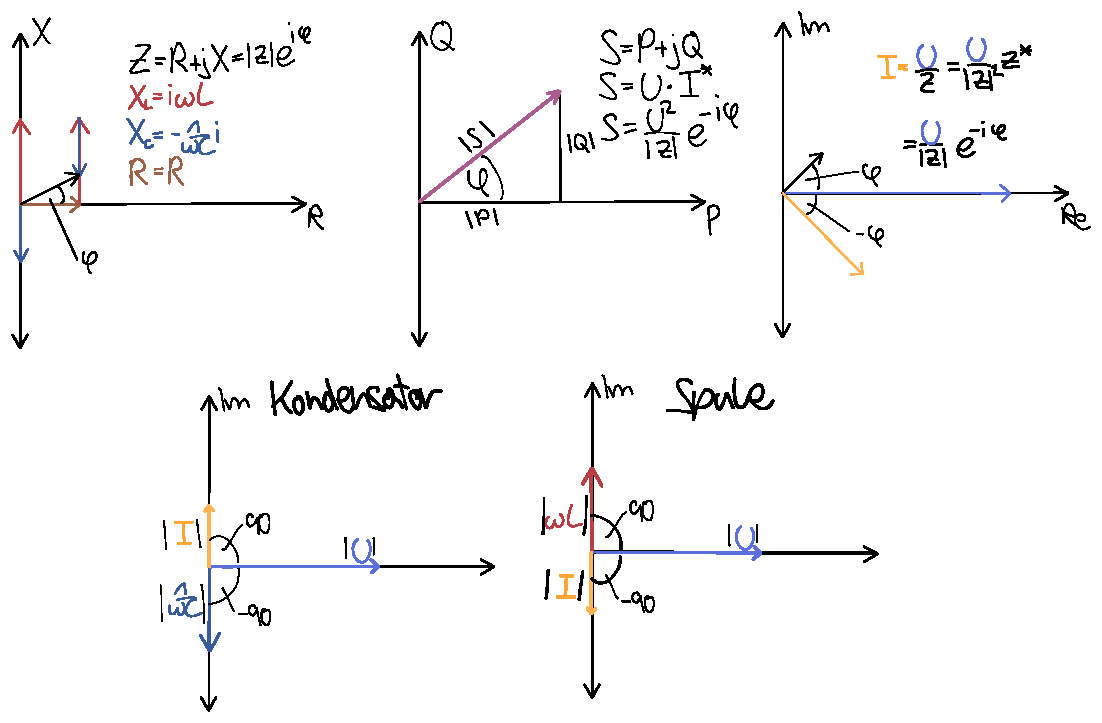
\includegraphics[width=0.95\textwidth]{./figures/grundlagen_zeiger.pdf}
	\end{center}
	\caption{Hier sind die Grundlagen der Zeigerdiagramme für Komplexe
		Wechselstromrechnung kurz und knapp in einem Diagramm dargestellt worden. Die
		Symbole entsprechen den zuvor definierten. \cite{gerthsen}}
	\label{fig:grundlagenzeiger}
\end{figure}
\vspace{5mm}

\section{Versuchsanordnung}\label{sec:Versuchsanordnung}

Im Rahmen dieses Versuchs wurden verschiedene Schaltungen dimensioniert. Eine jeweilige Skizze des Schaltplans und eine kurze Erklärung finden sich, der besseren Übersicht halber, immer am Anfang des entsprechenden Versuchs im \autoref{sec:Versuchsdurchführung}.

\vspace{2mm}

Um die Signale für die entsprechenden Schaltpläne zu Erzeugen und Auszuwerten wurden folgende Geräte verwendet.

\vspace{2mm}

Es handelt sich dabei um einen ``Power Supply``, in \autoref{fig:hameg} und ein Oszilloskop, siehe \autoref{fig:oszi}

\vspace{2mm}

\begin{minipage}{\textwidth}
	\begin{minipage}[t]{0.5\textwidth}
		\centering
		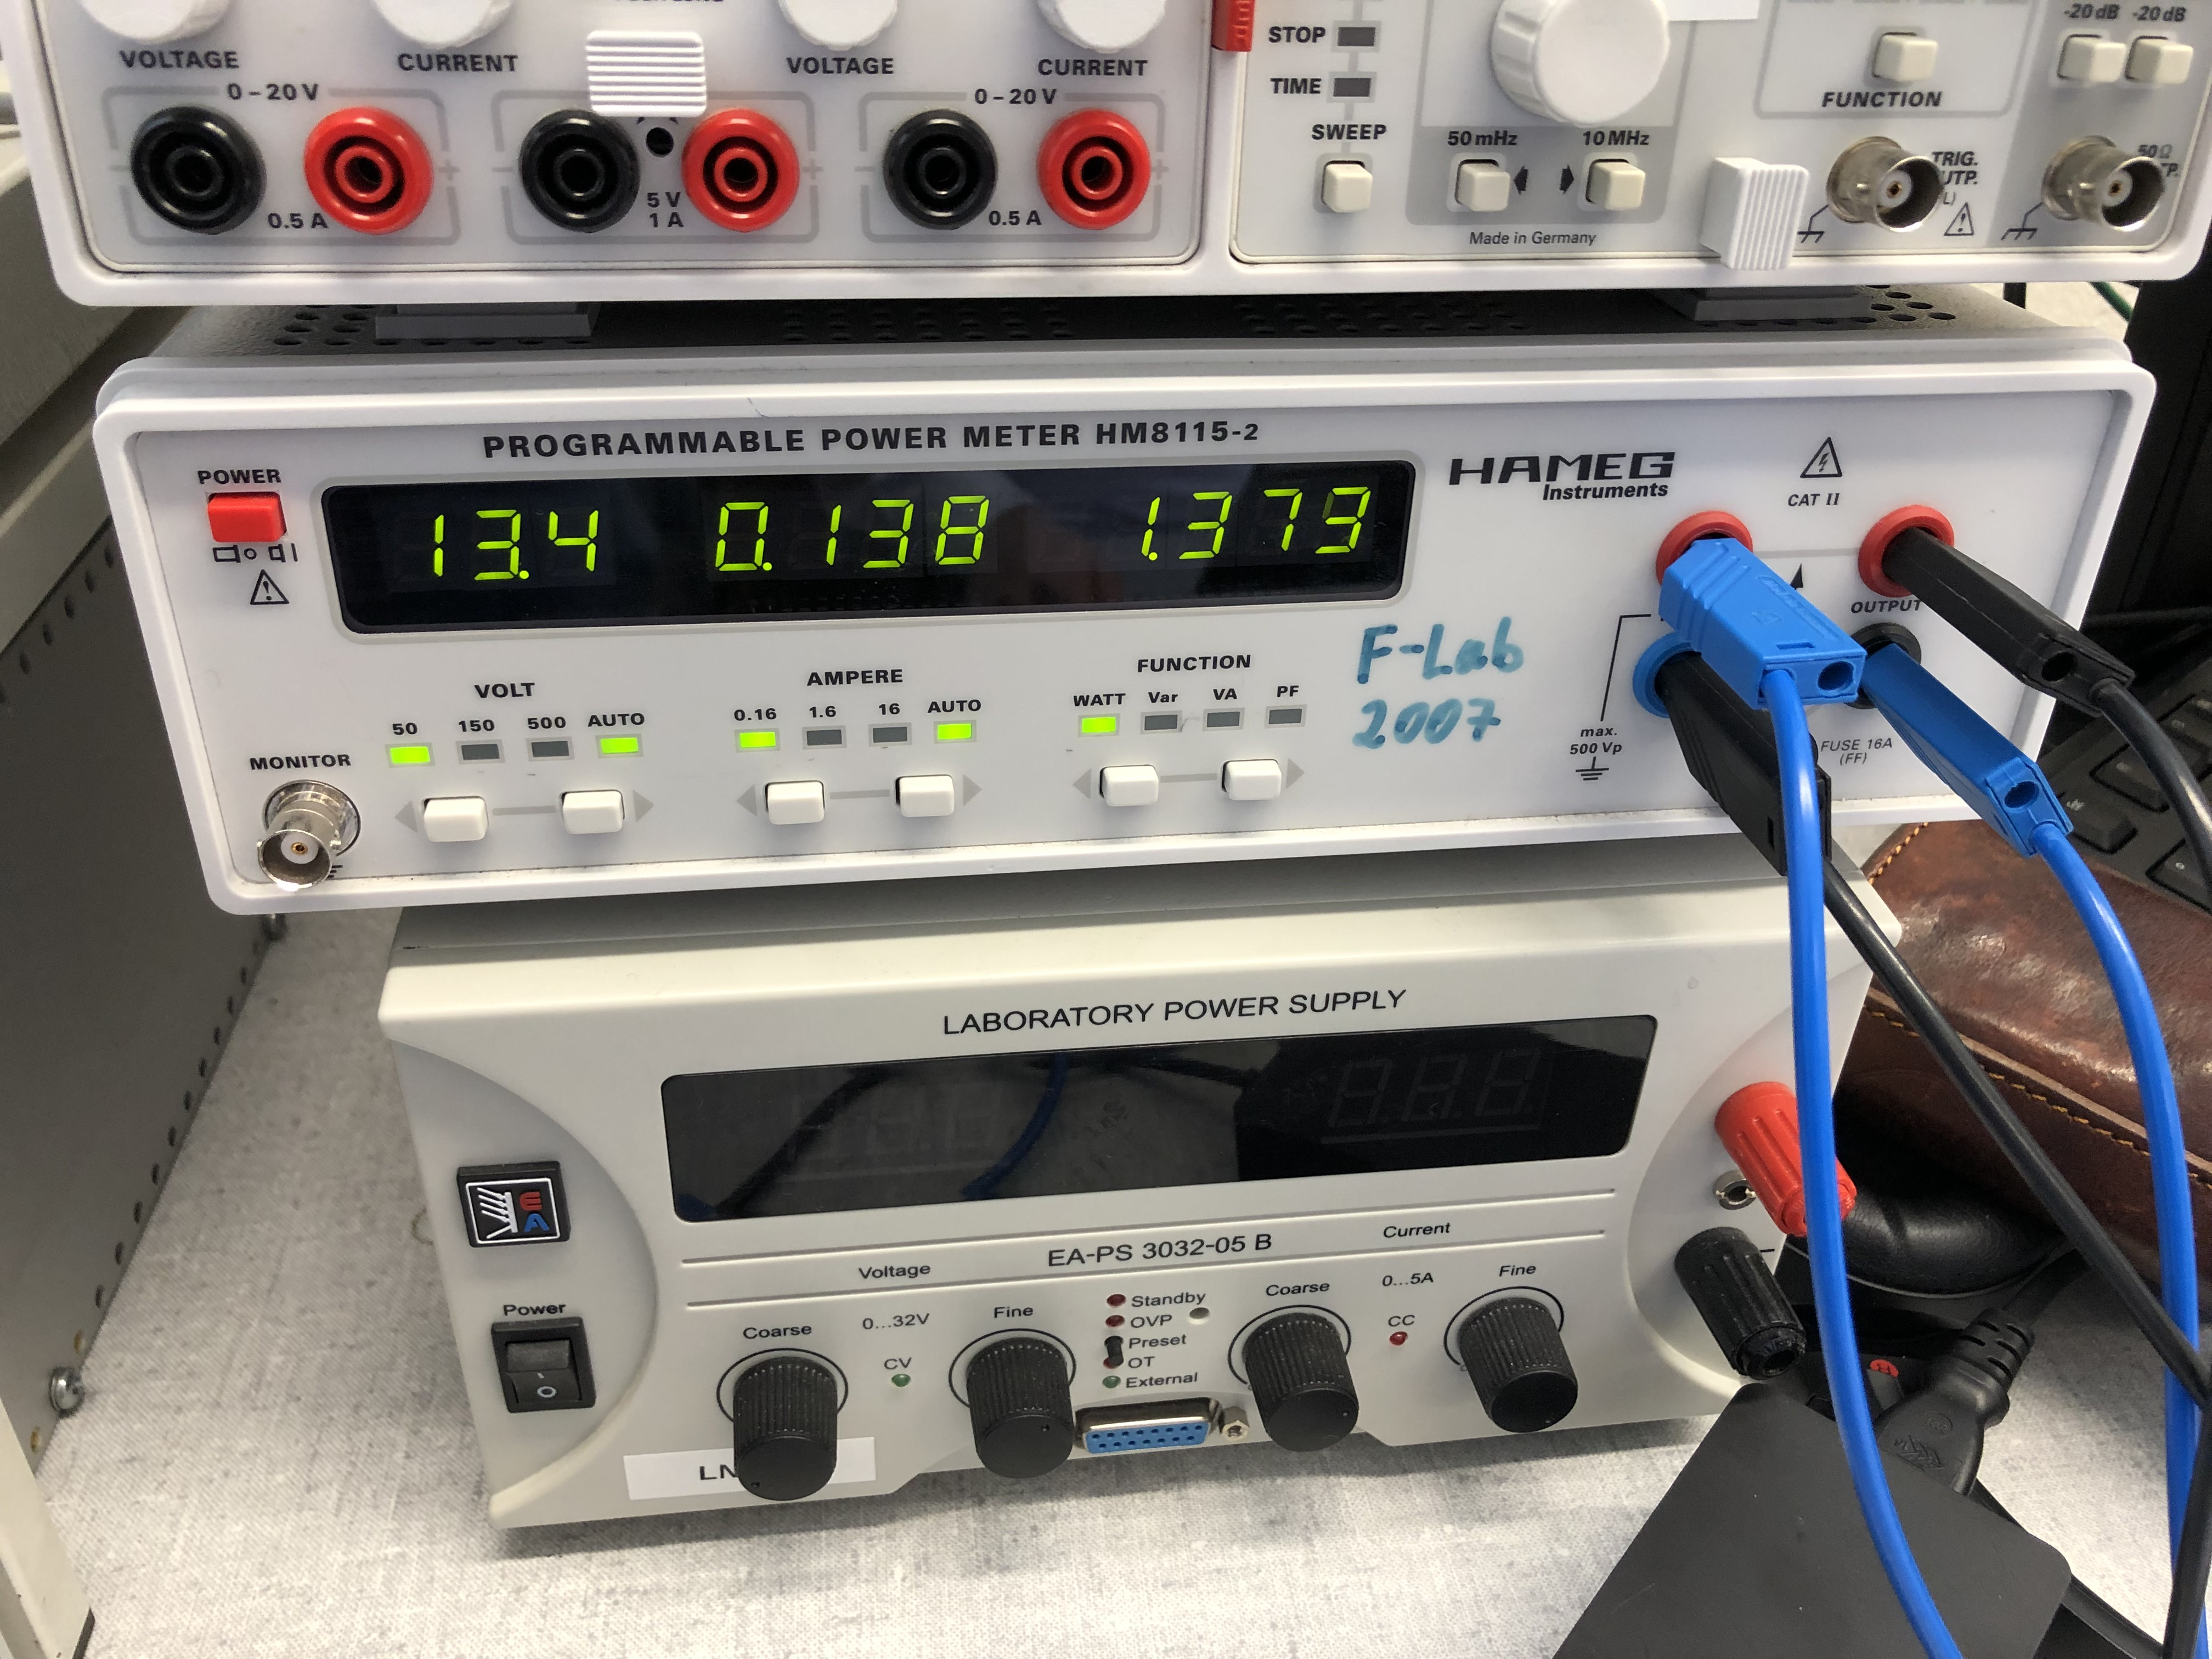
\includegraphics[width=\textwidth]{hameg}
		\captionbelowof{figure}{Verwendeter ``Power Supply``}
		\label{fig:hameg}
	\end{minipage}
	\vspace{2mm}
	\begin{minipage}[t]{0.50\textwidth}
		\centering
		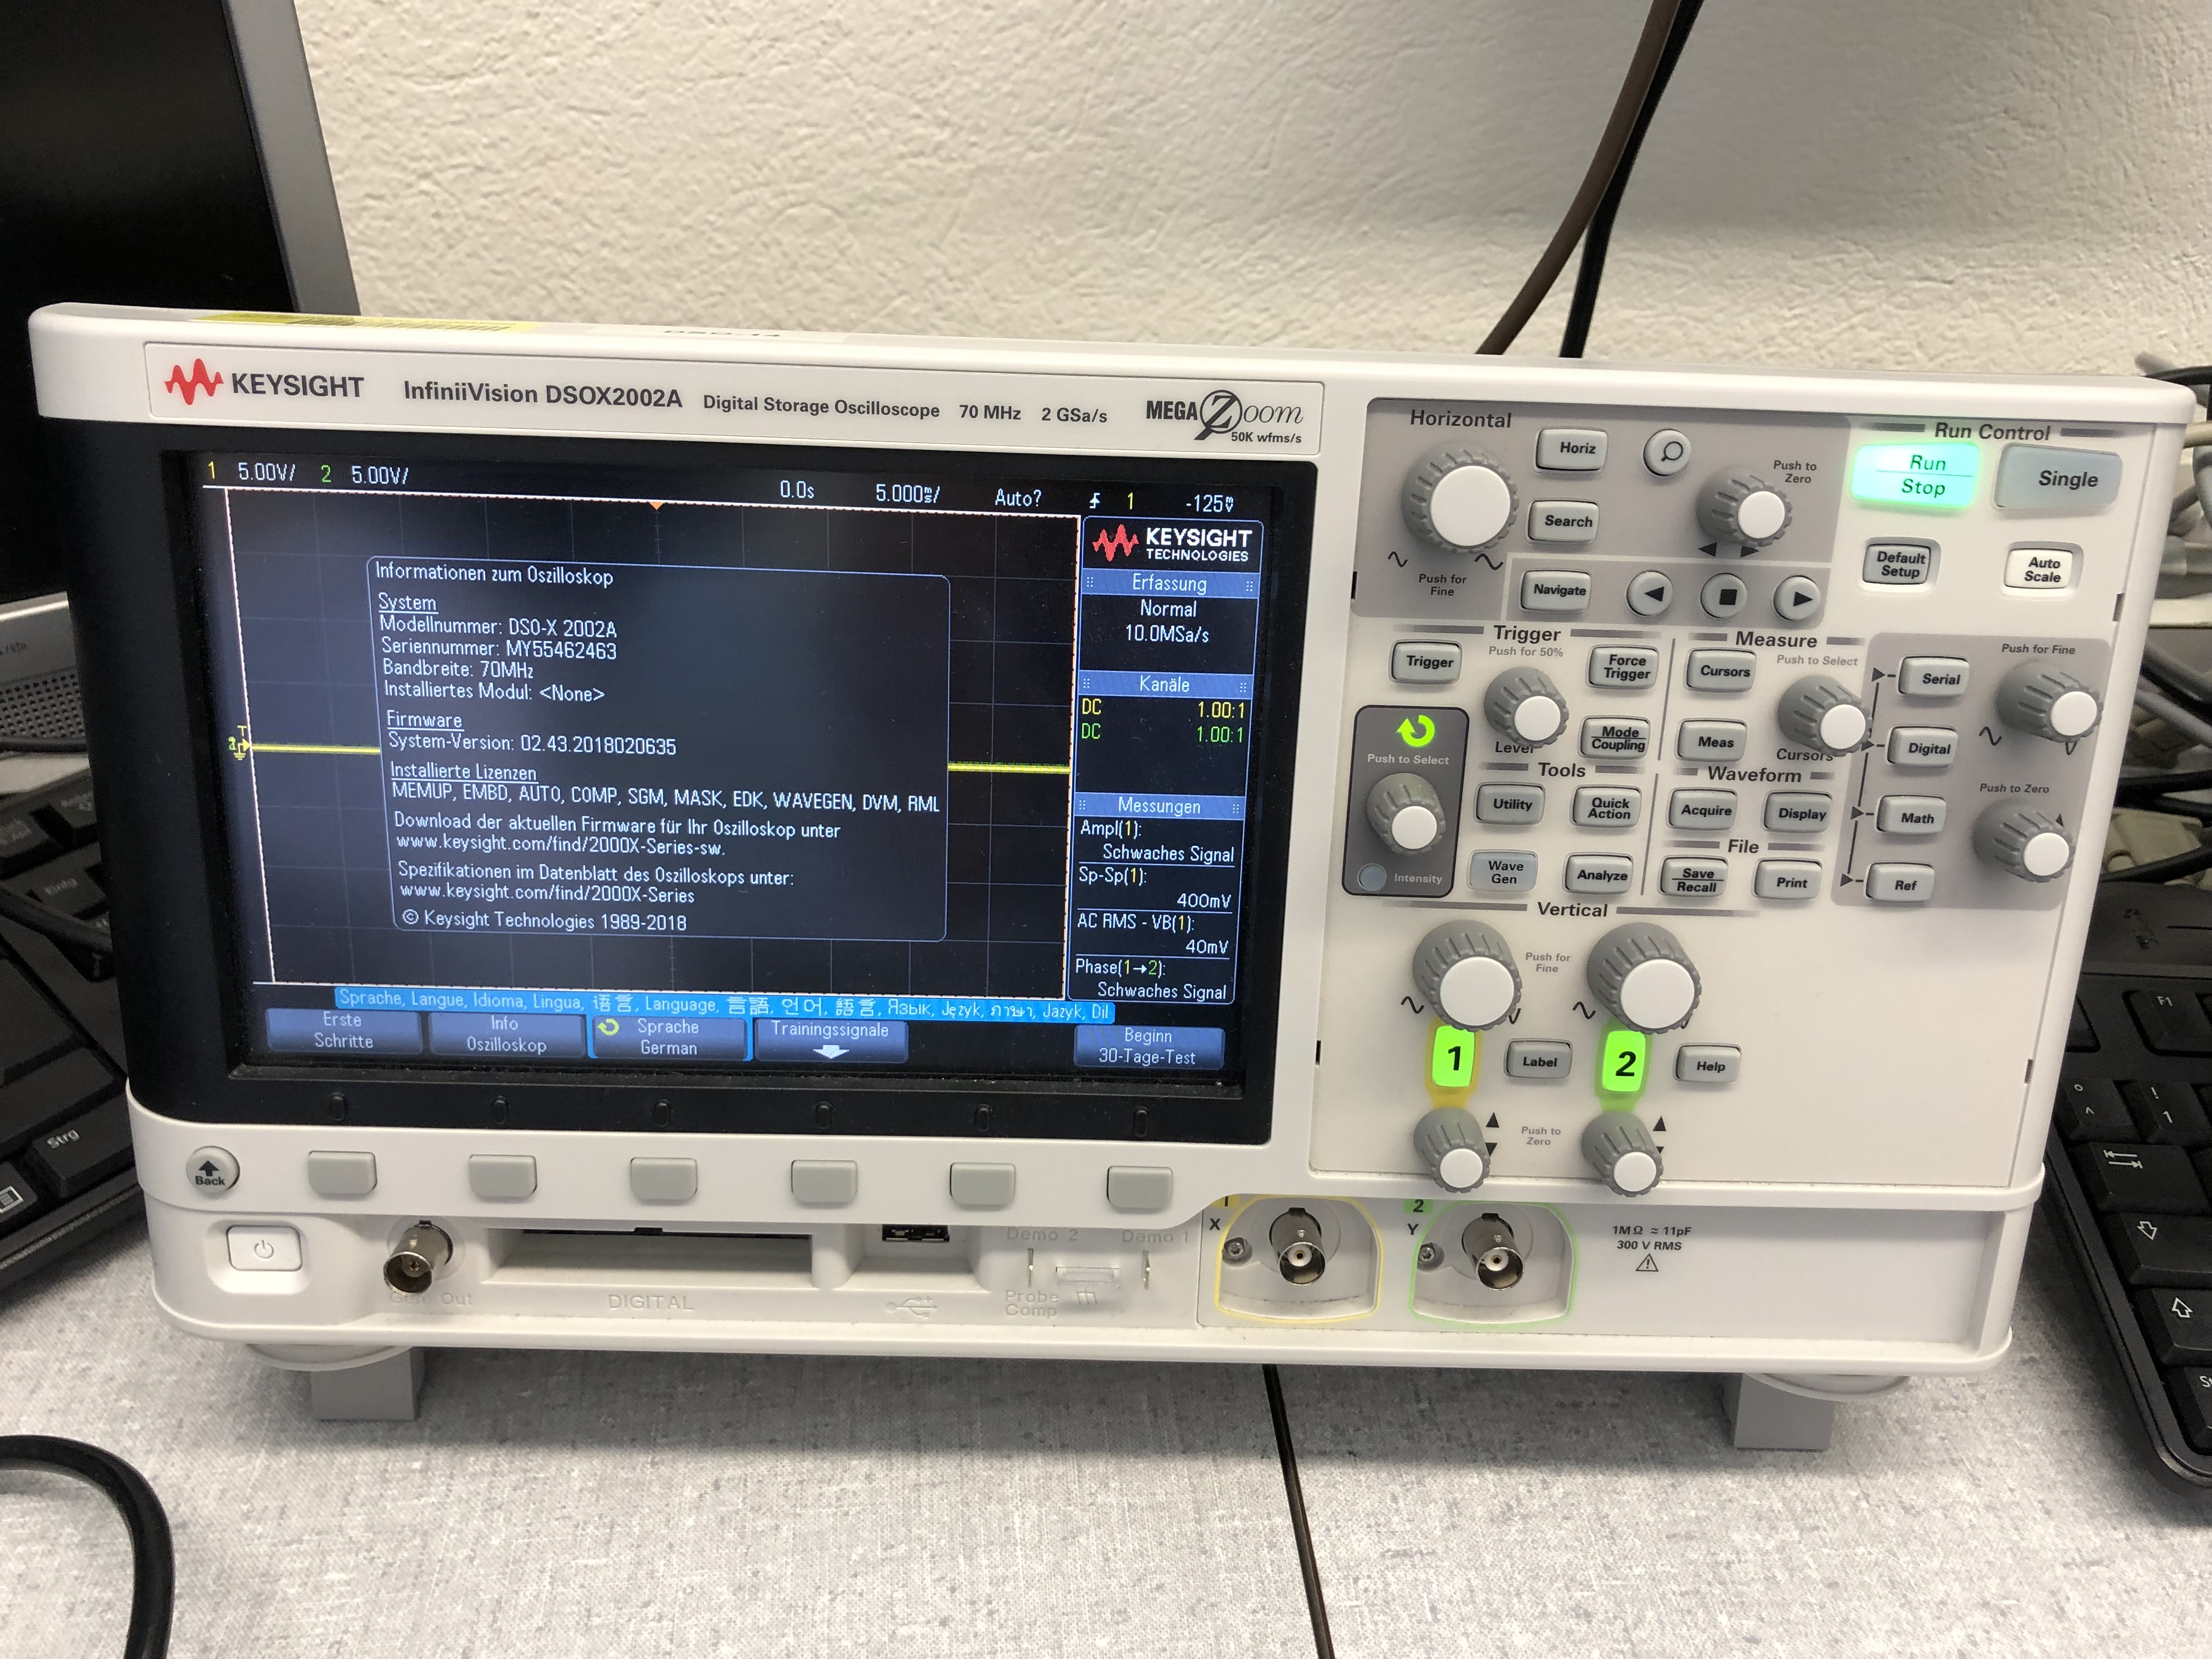
\includegraphics[width=\textwidth]{oszi}
		\captionof{figure}{Verwendetes Oszilloskop}
		\label{fig:oszi}
	\end{minipage}
	\vspace{1em}
\end{minipage}

\newpage

Zusätzlich wurden ein Transformator, siehe \autoref{fig:transf} und digitales Multimeter, siehe \autoref{fig:multi_dig}, verwendet.

\begin{minipage}{\textwidth}
	\begin{minipage}[t]{0.5\textwidth}
		\centering
		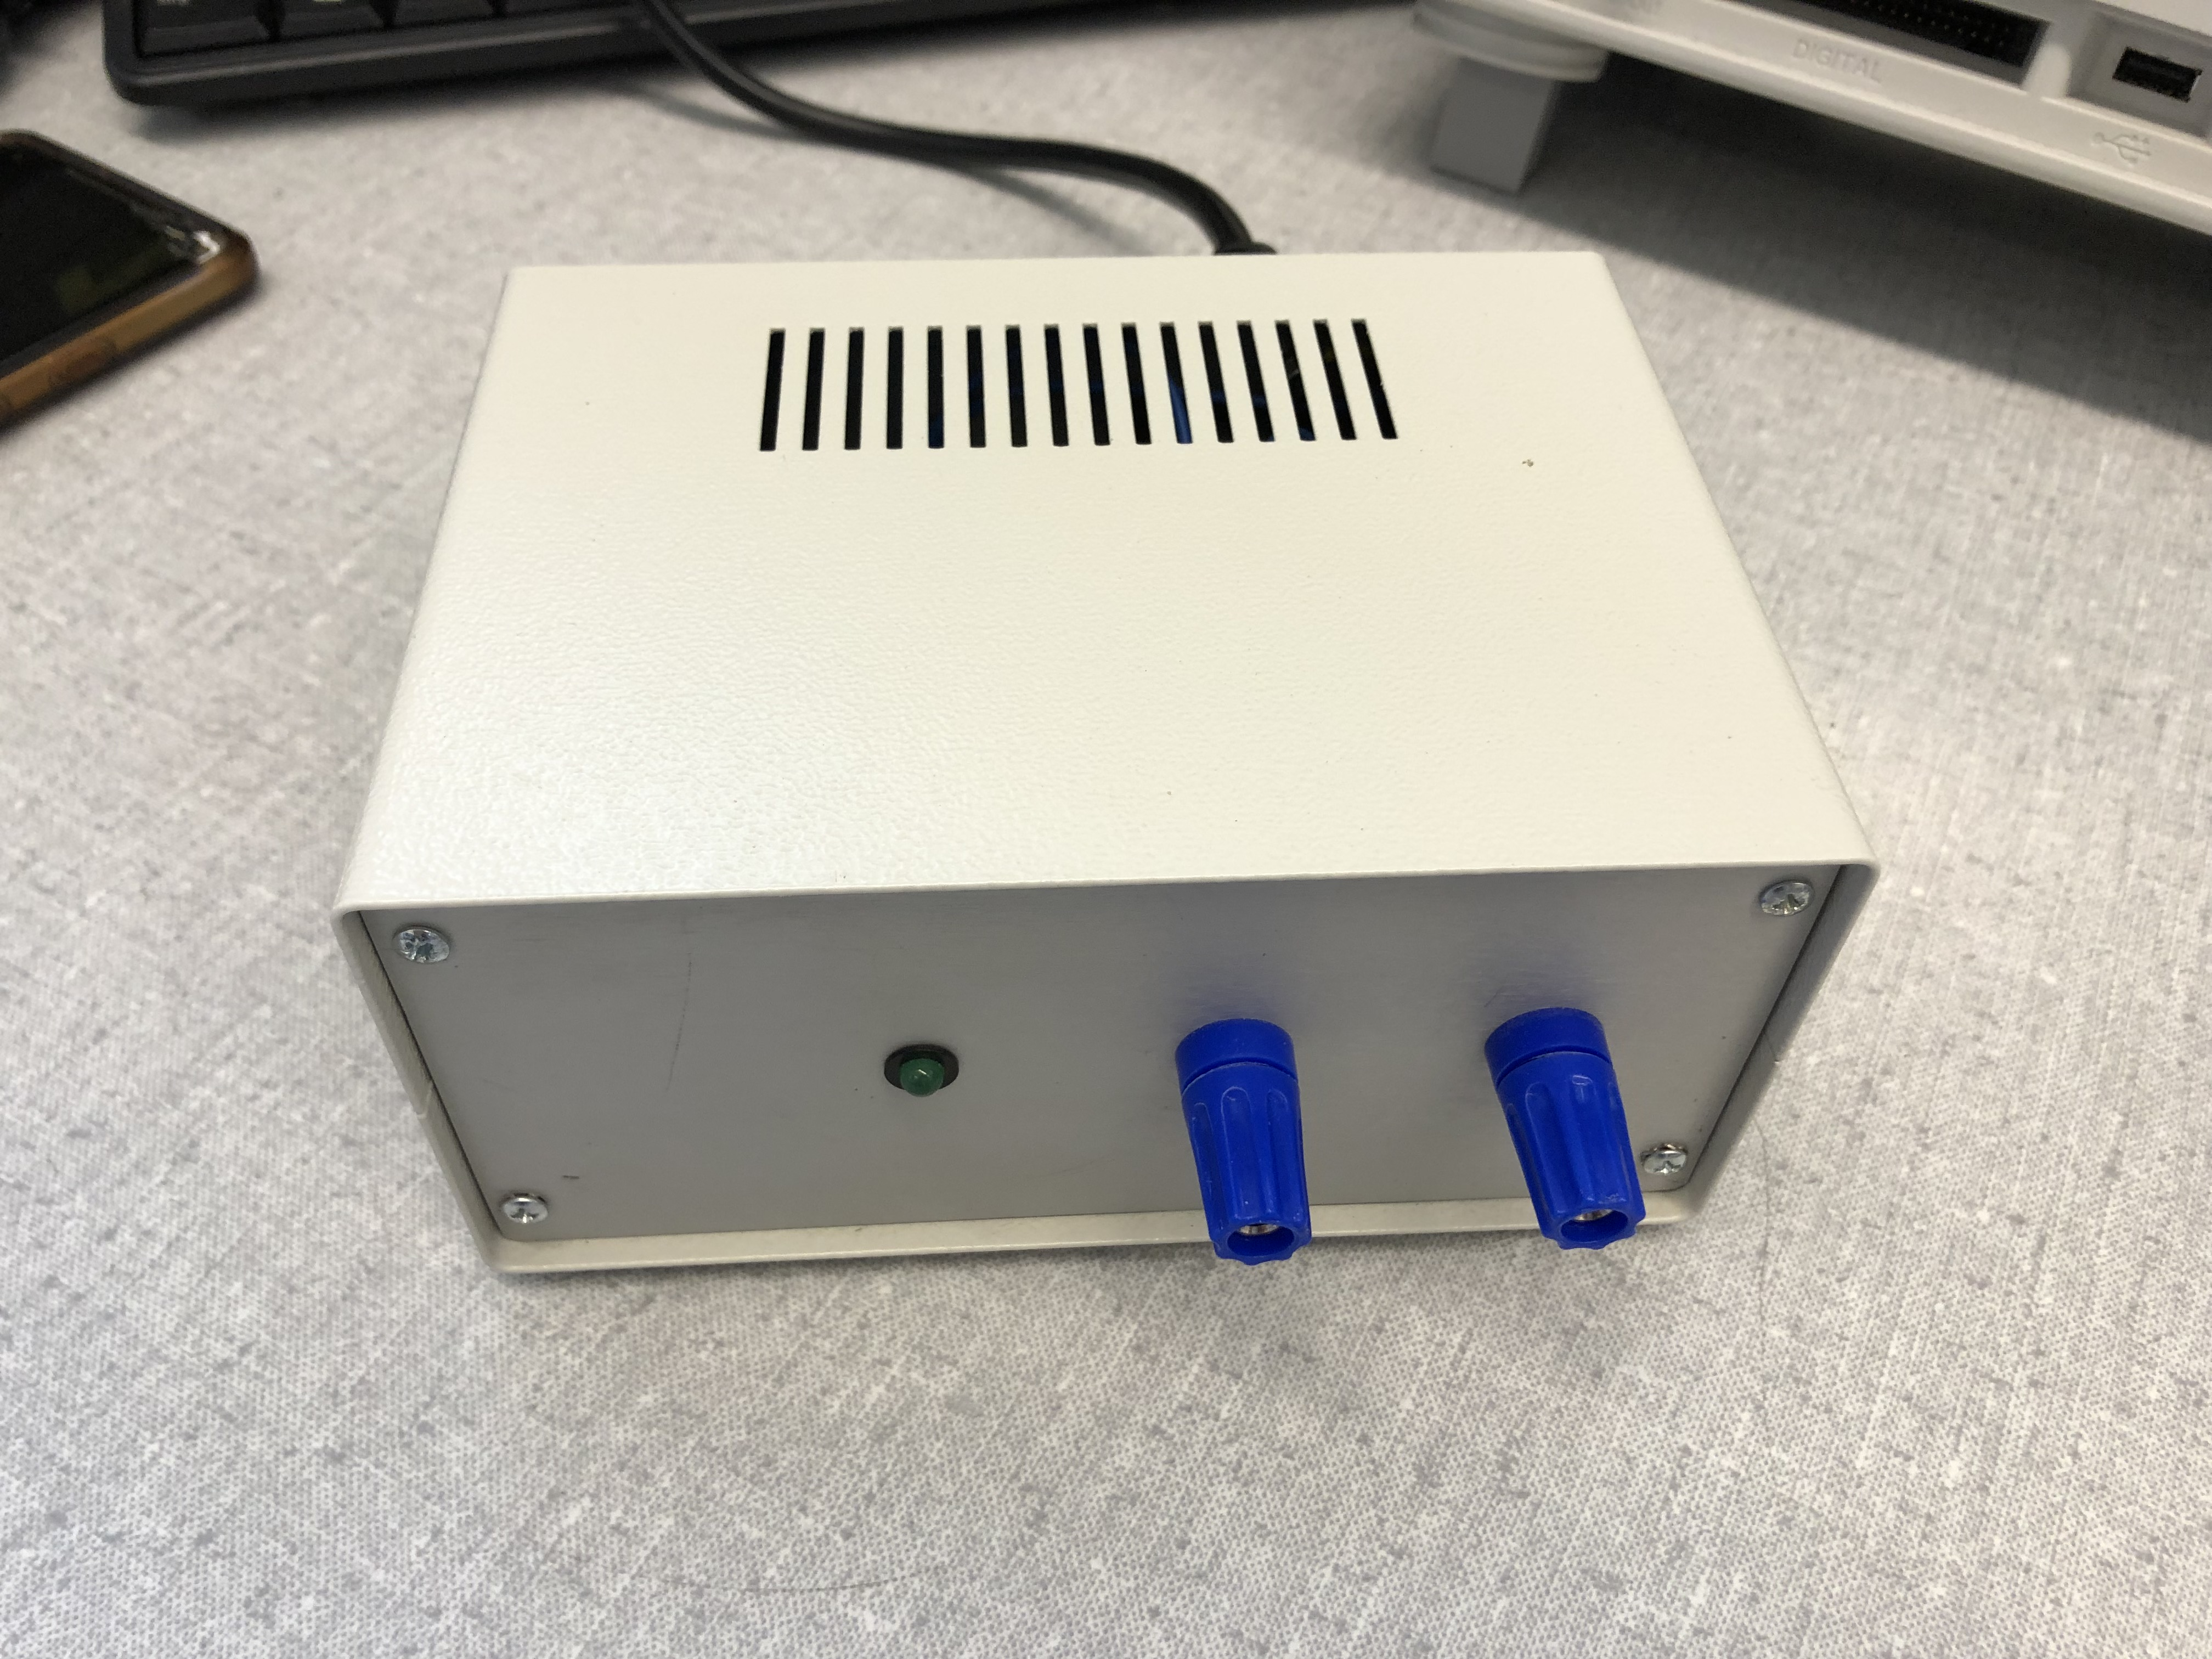
\includegraphics[width=\textwidth]{trafo}
		\captionbelowof{figure}{Verwendeter Trafo}
		\label{fig:transf}
	\end{minipage}
	\vspace{2mm}
	\begin{minipage}[t]{0.5\textwidth}
		\centering
		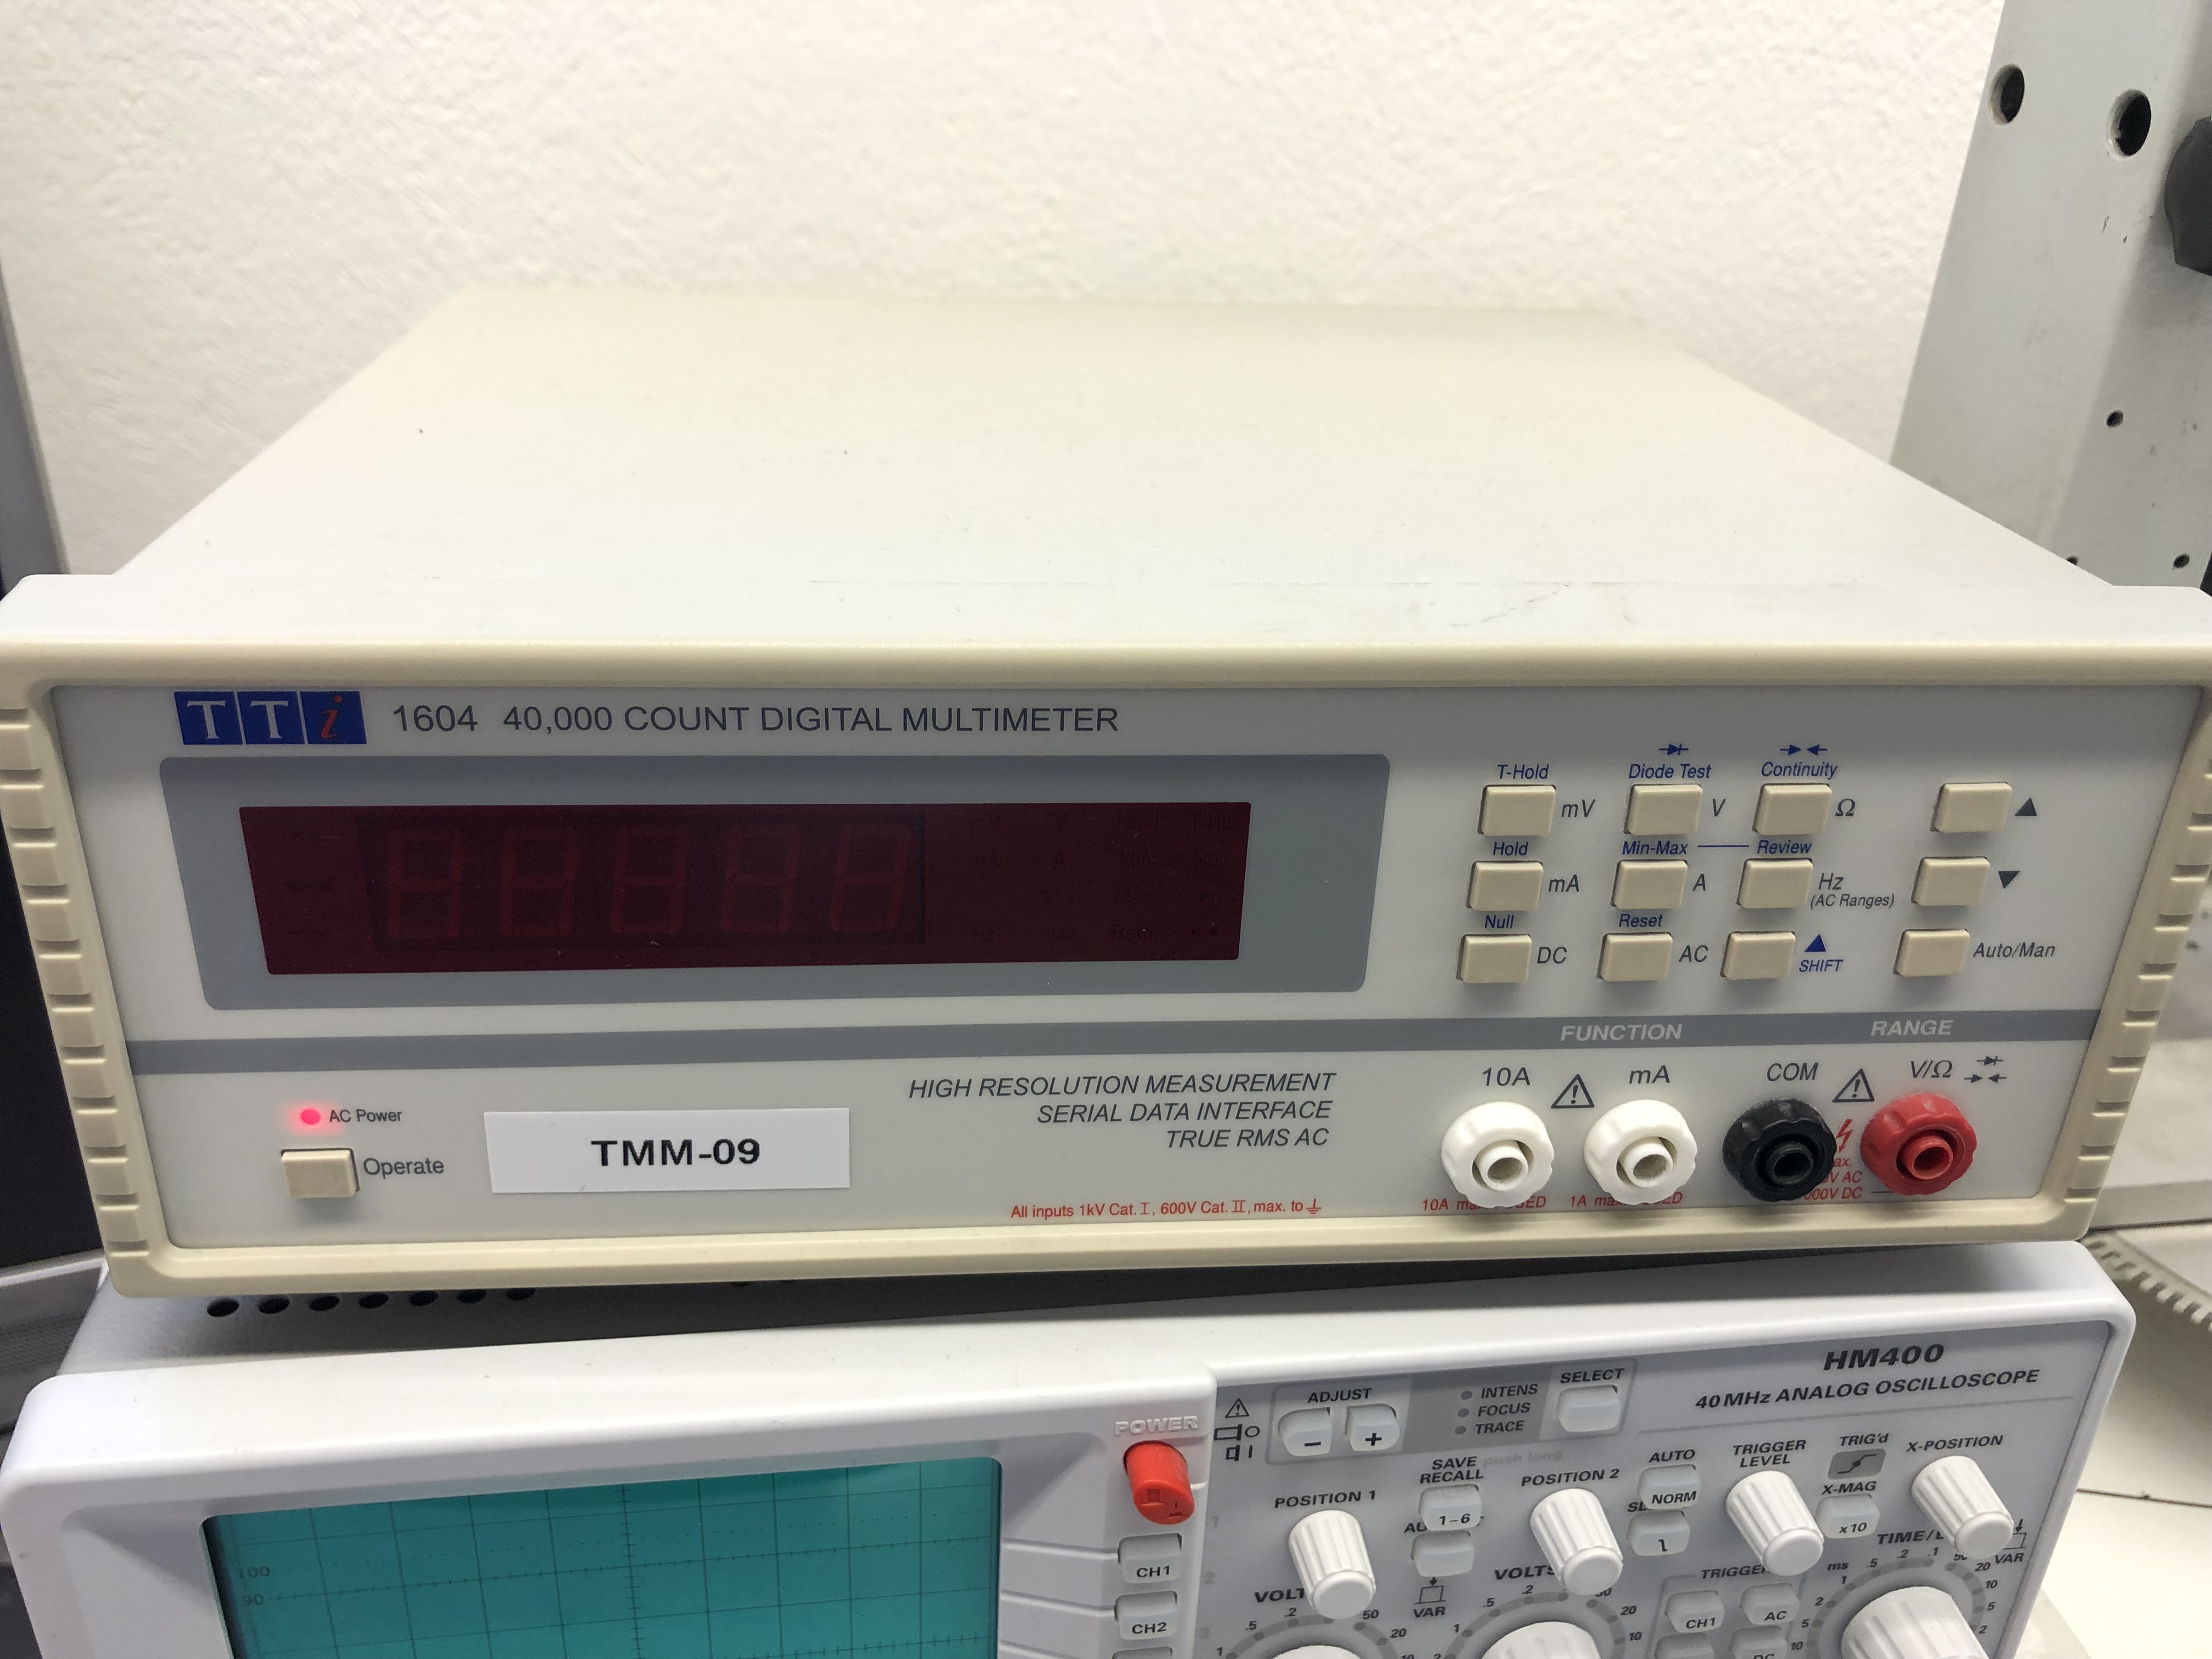
\includegraphics[width=\textwidth]{multi_dig}
		\captionof{figure}{Verwendetes digitales Multimeter}
		\label{fig:multi_dig}
	\end{minipage}
	\vspace{1em}
\end{minipage}

Zusätzlich zum digitalen Multimeter aus \autoref{fig:multi_dig} werden auch noch herkömmliche Multimeter der Firma FLUKE, rechts in \autoref{fig:multi} und eine etwas billigere Version eines digitalen Multimeters, links in \autoref{fig:multi}, verwendet. Auch steht ein analoges Multimeter zur Verfügung, siehe \autoref{fig:multi_alt}.

\begin{minipage}{\textwidth}
	\begin{minipage}[t]{0.5\textwidth}
		\centering
		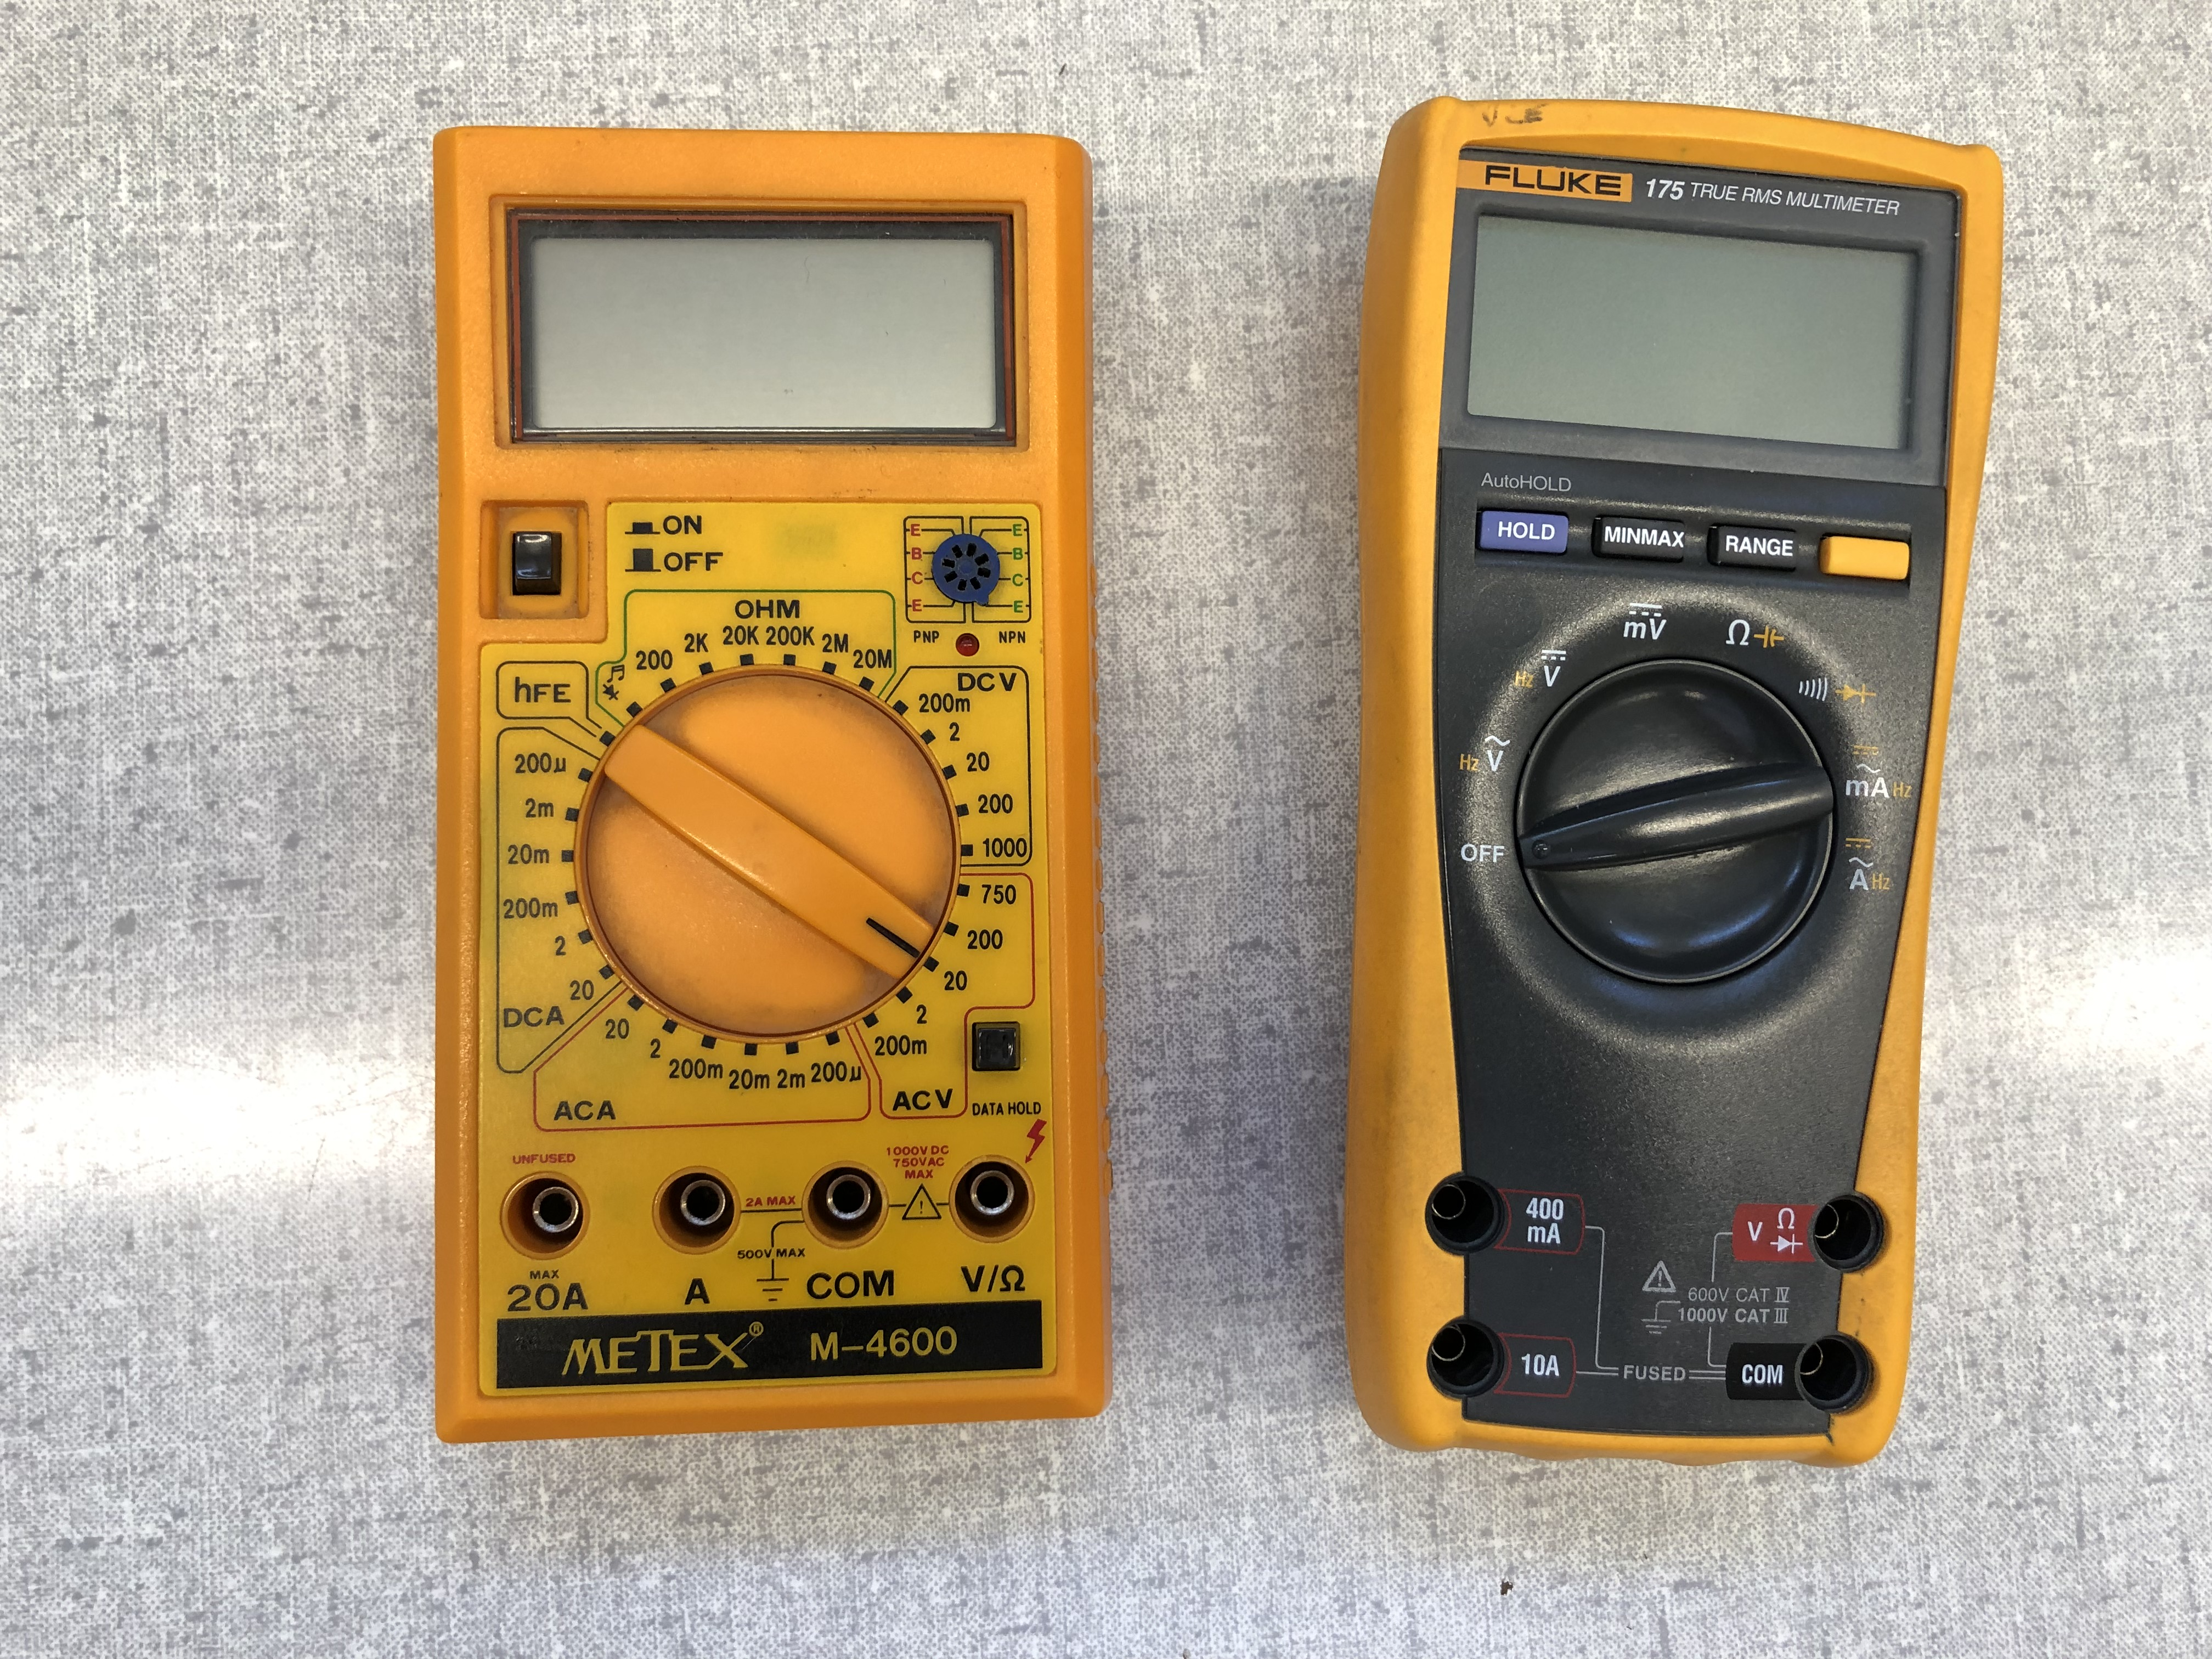
\includegraphics[width=\textwidth]{multi}
		\captionbelowof{figure}{Verwendeter Multimeter der Marken Metex und Fluke}
		\label{fig:multi}
	\end{minipage}
	\vspace{2mm}
	\begin{minipage}[t]{0.5\textwidth}
		\centering
		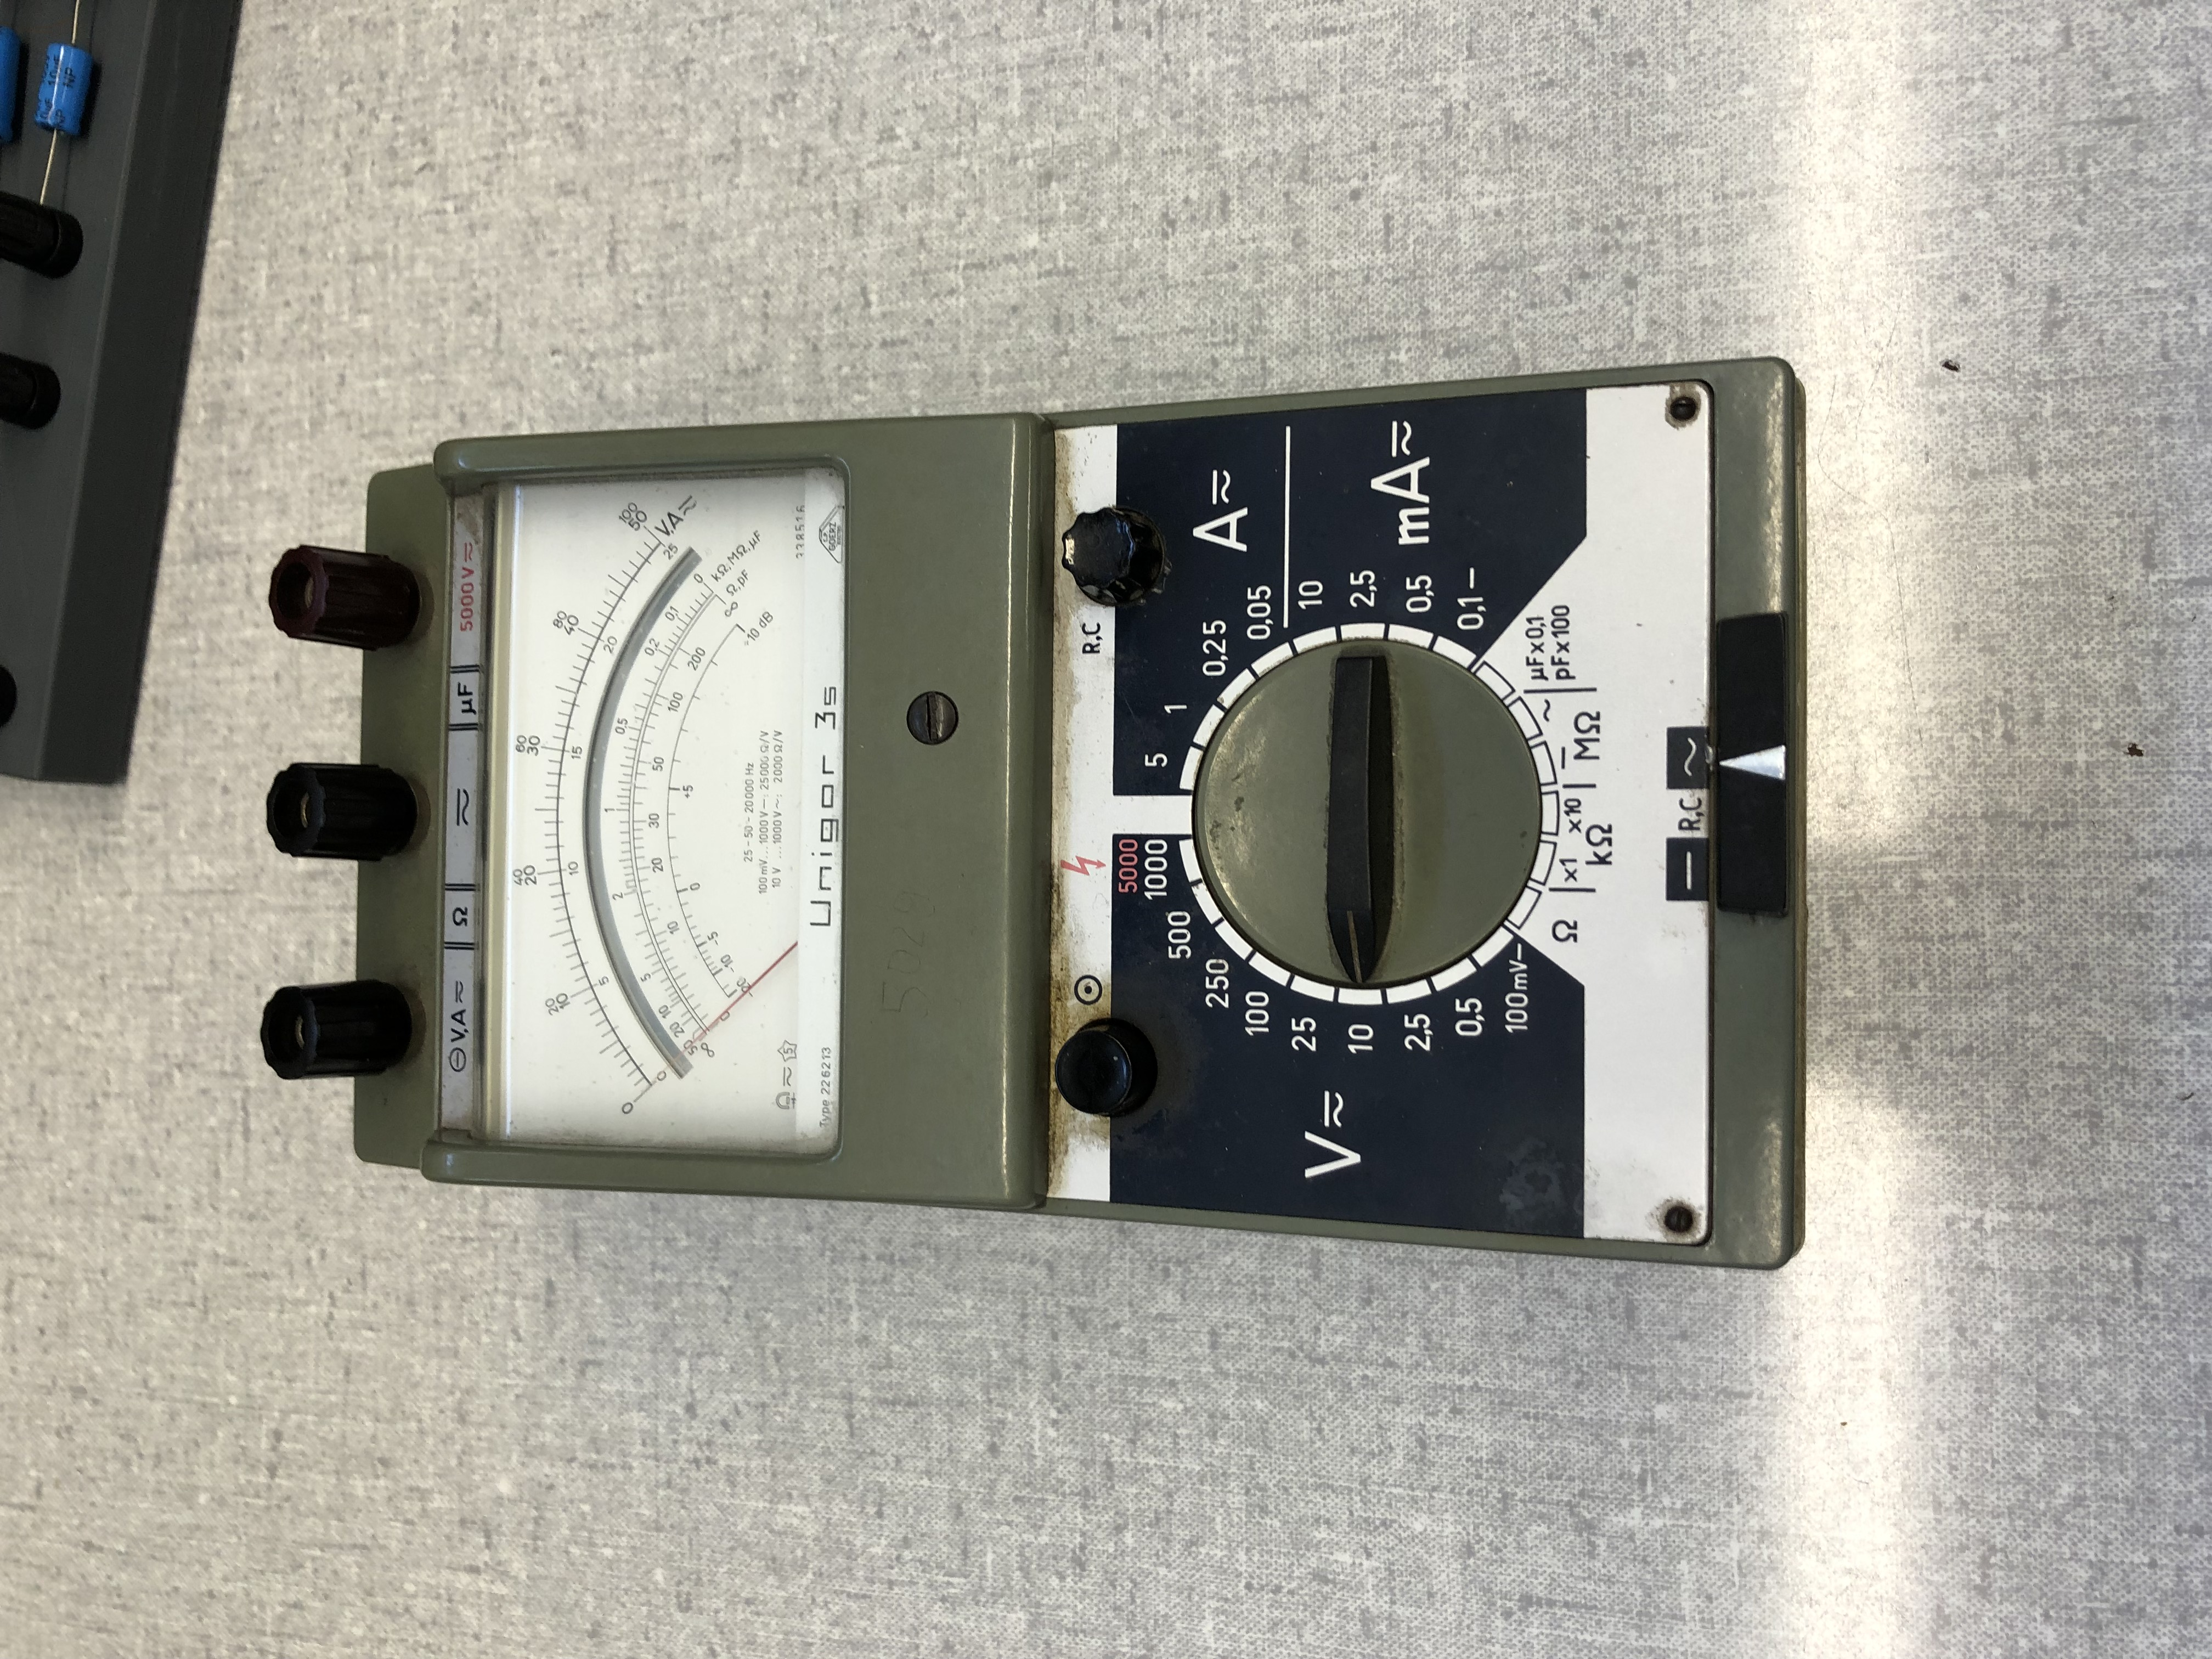
\includegraphics[angle=270,width=\textwidth]{multi_alt}
		\captionof{figure}{Verwendetes analoges Multimeter}
		\label{fig:multi_alt}
	\end{minipage}
	\vspace{1em}
\end{minipage}

Für den Versuchsaufbau wird außerdem eine Spule, (1) in \autoref{fig:steck}, verwendet. Zusätzlich wird ein Widerstand von 66.76 $\Omega$ für den Versuchsaufbau benötigt, markiert mit (2) in \autoref{fig:steck}. Auch werden Kondensatoren mit verschiedenen Kapazitäten benötigt. In \autoref{fig:steck} handelt es sich dabei um Kondensatoren mit Kapazitäten von 100 $\mu$ Farad (3), 47 $\mu$ Farad (4), 20 $\mu$ Farad (5) und 10 $\mu$ Farad (6).

Um die verschiedenen Schaltungen zu realisieren, werden normale Steckkabel verwendet. Um die Koaxialanschlüsse in den Stromkreis zu integrieren werden Tastkabel, sichtbar in \autoref{fig:tastkabel}, verwendet.

\begin{minipage}{\textwidth}
	\begin{minipage}[t]{0.5\textwidth}
		\centering
		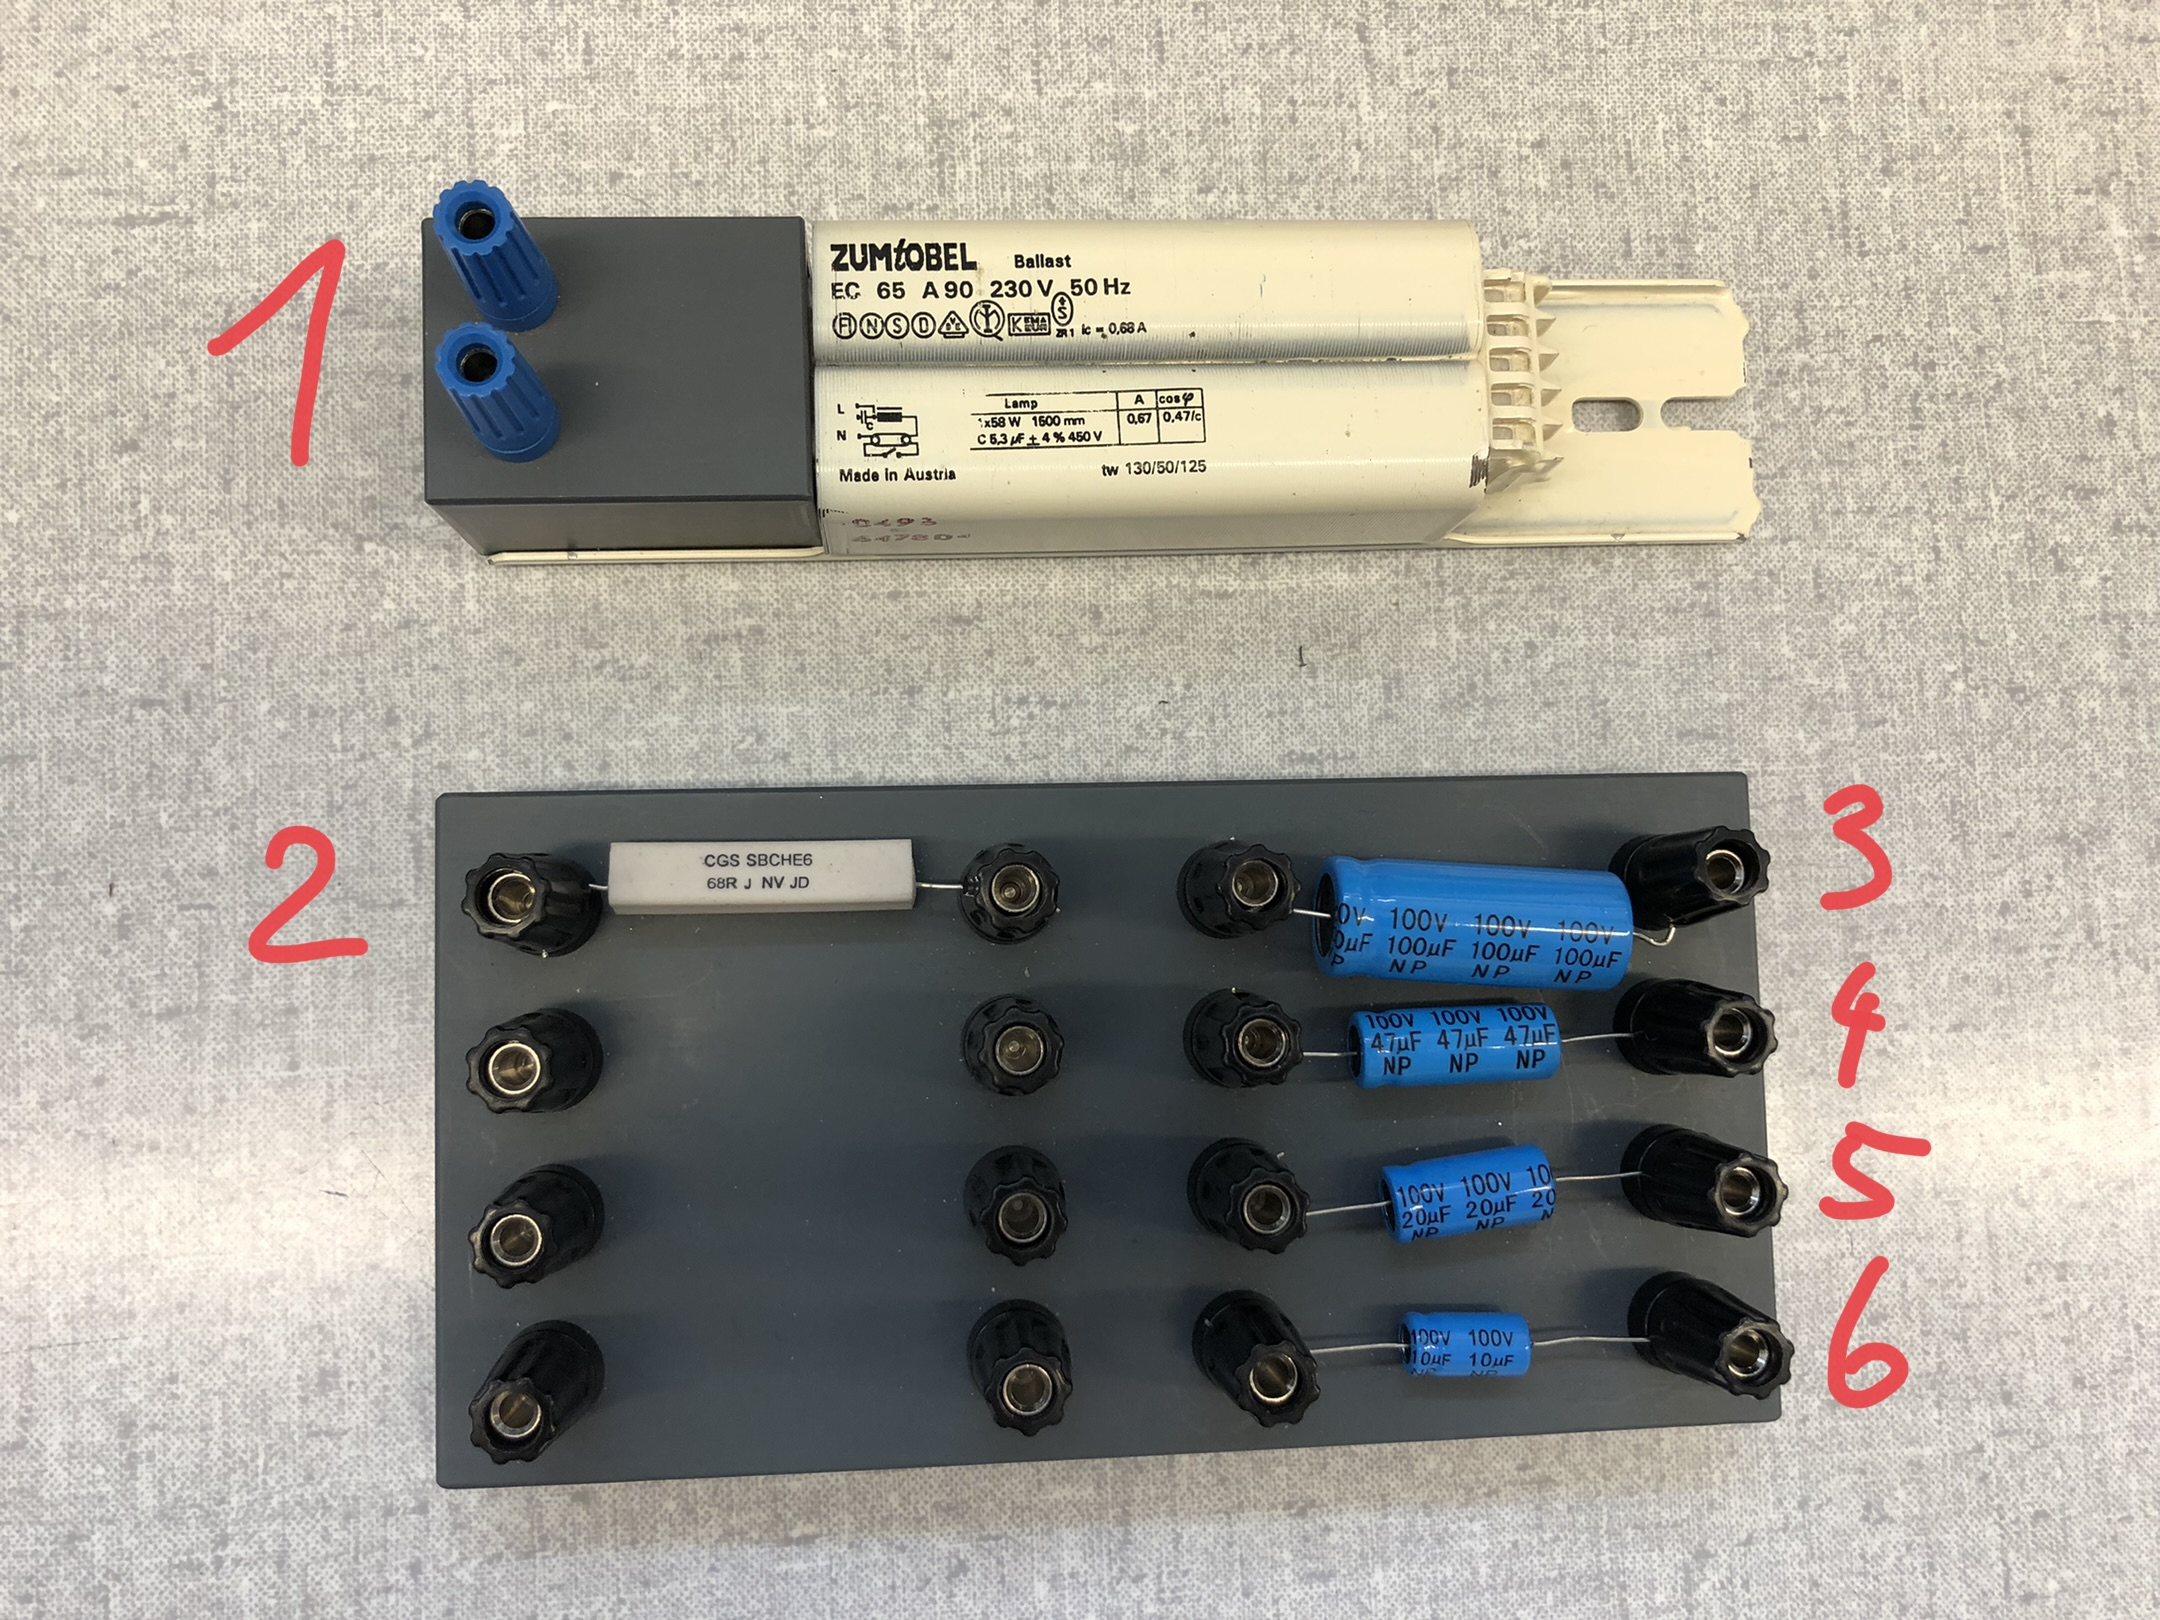
\includegraphics[width=\textwidth]{kapa}
		\captionbelowof{figure}{Verwendete Spule (1), Widerstand (2) und Kapazitäten}
		\label{fig:steck}
	\end{minipage}
	\vspace{2mm}
	\begin{minipage}[t]{0.5\textwidth}
		\centering
		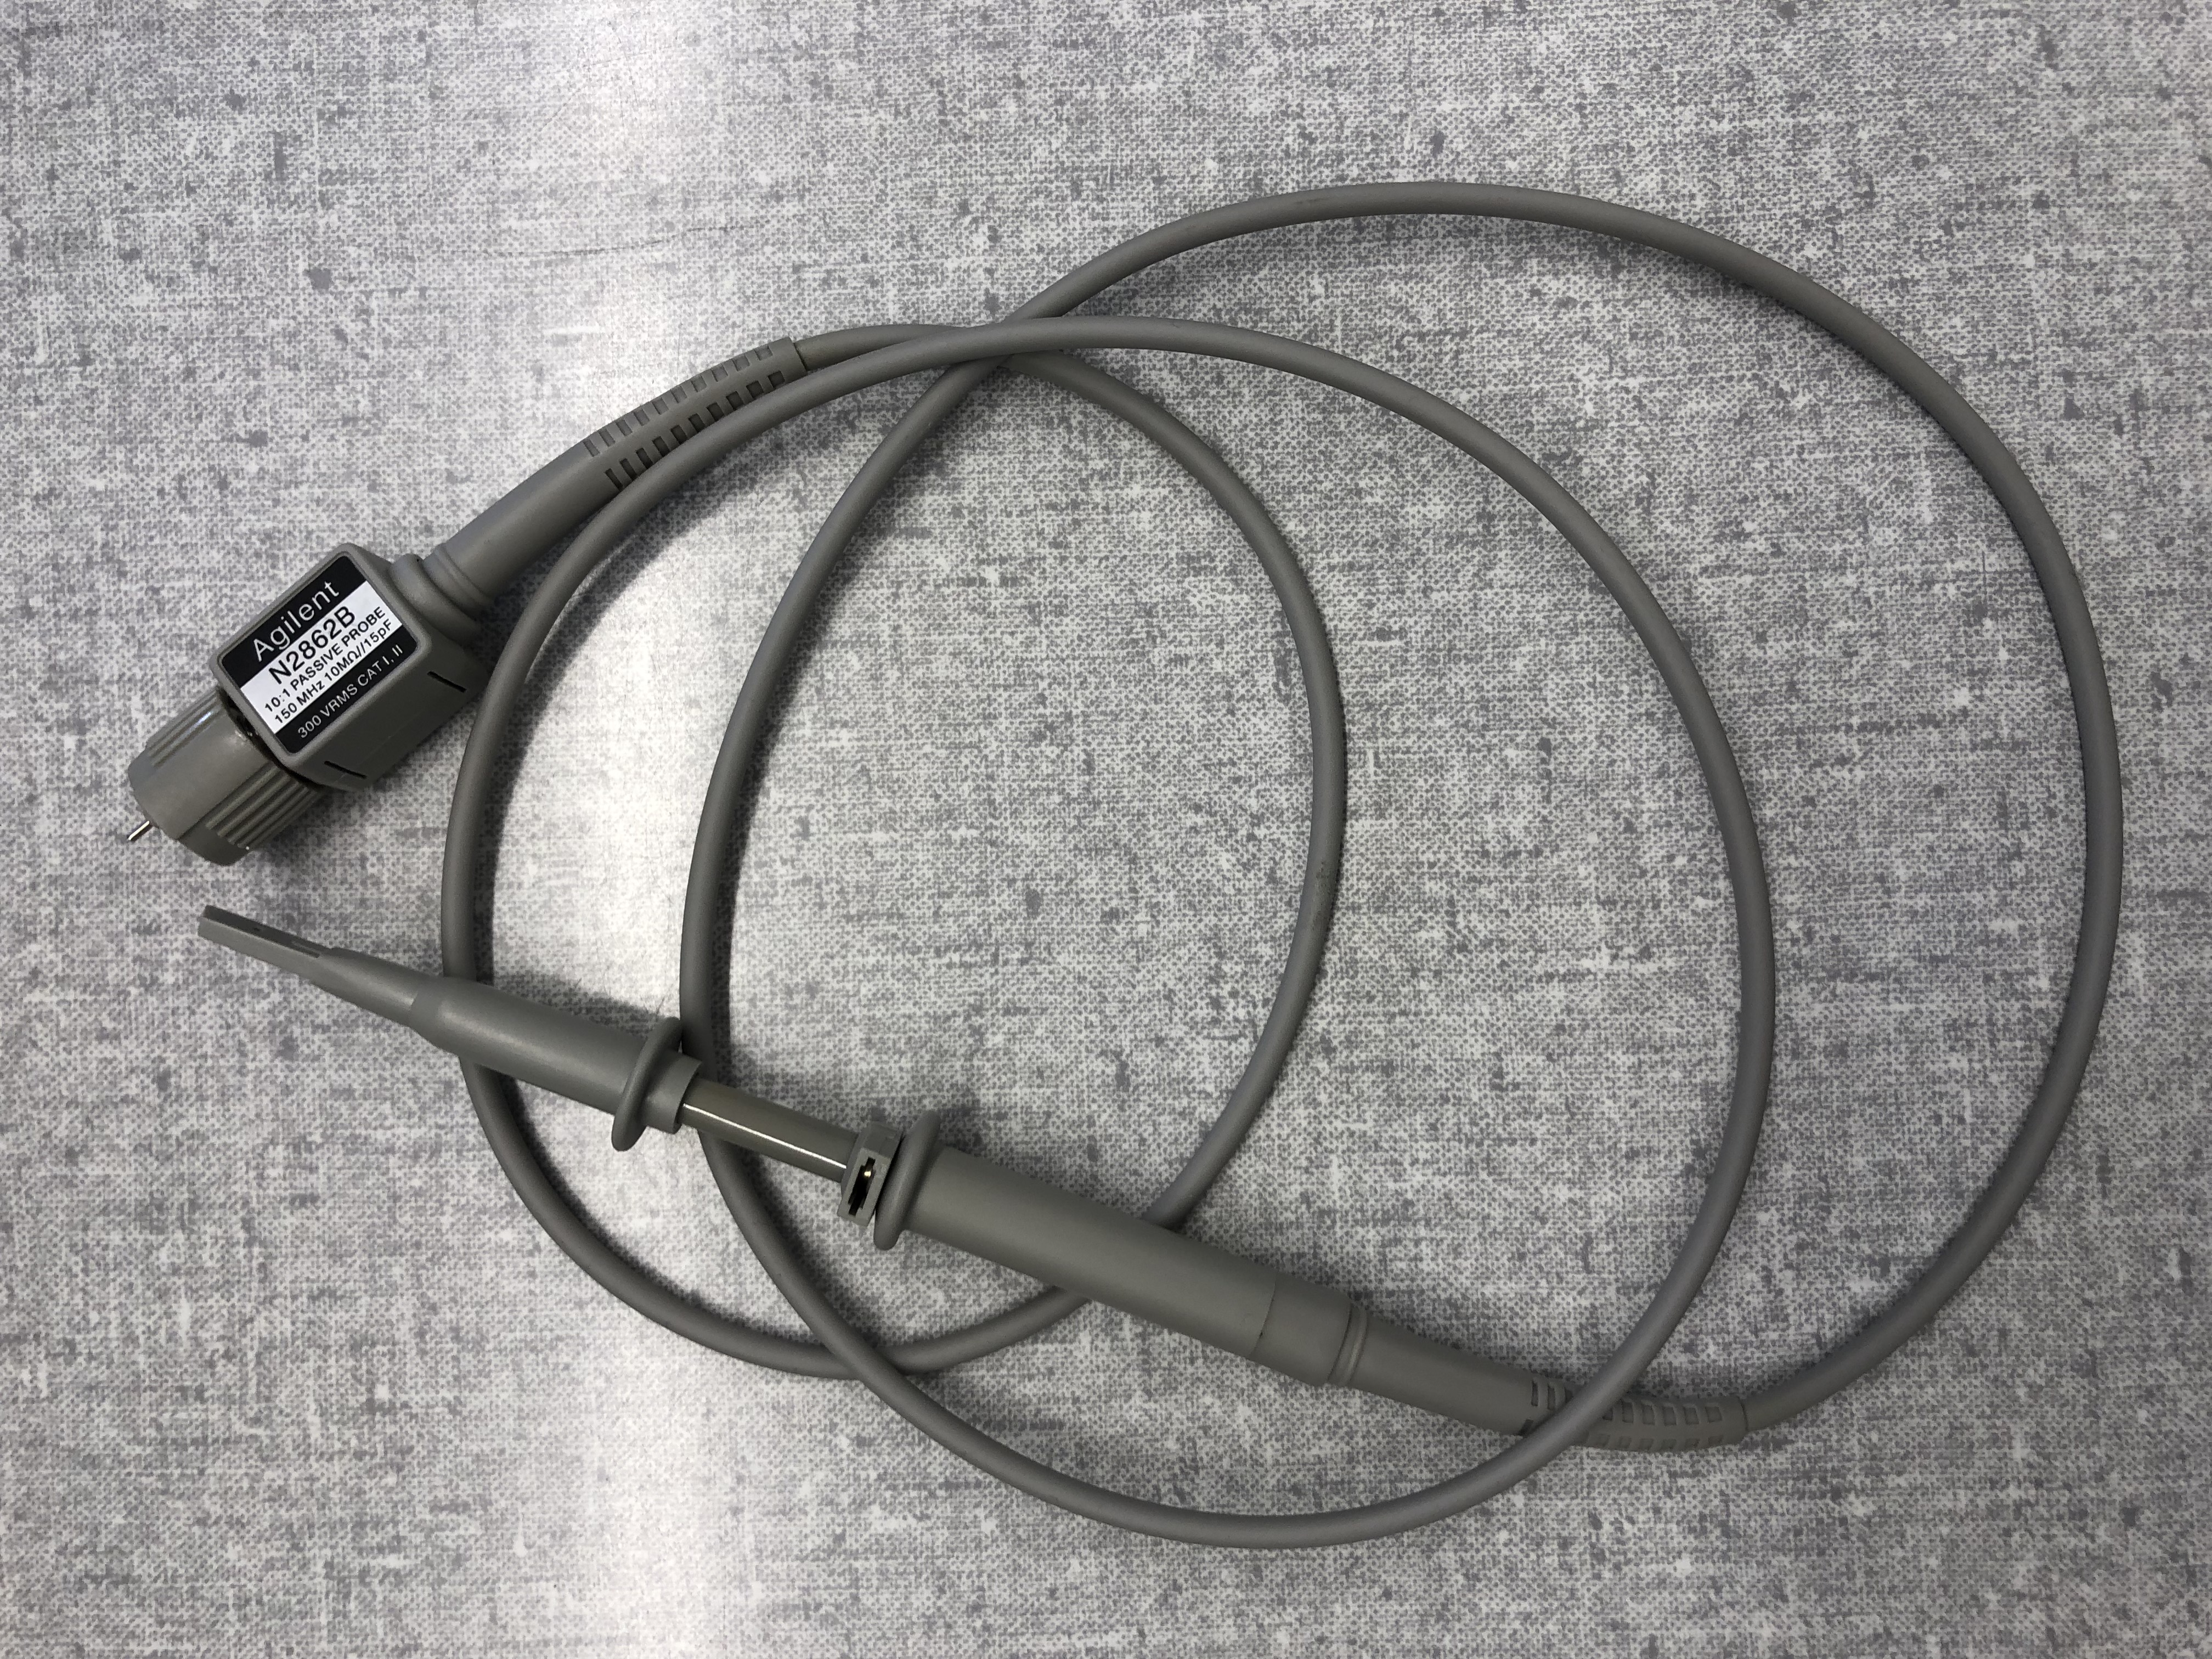
\includegraphics[width=\textwidth]{tastkabel}
		\captionof{figure}{Verwendete Tastkabel}
		\label{fig:tastkabel}
	\end{minipage}
	\vspace{1em}
\end{minipage}



\section{Geräteliste}

\noindent Für die Messungen wurden folgende Geräte verwendet:

\captionof{table}{Verwendete Geräte}
\begin{center}
	\begin{tabular}{|c|c|c|c|c|} \hline
		\textbf{Gerät}       & \textbf{Typ}         & \textbf{Hersteller} & \textbf{Seriennummer} \\ \hline

		Oszilloskop          & DSO-X 2002A          & Keysight            & MY55462463            \\ \hline
		``Power Supply``     & HM 8115-2            & Hameg Instruments   & F-Lab 2007            \\ \hline
		Digitales Multimeter & 1604 40,000 Count    & TTi                 & TMM-05                \\ \hline
		Multimeter           & M-4600               & METEX               &                       \\ \hline
		3 Multimeter         & 175 True RMS         & Fluke               &                       \\ \hline
		analoges Multimeter  & 3s                   & Unigor              & F                     \\ \hline
		Transformator        &                      &                     &                       \\ \hline
		Kabel                & 60 V DC 16 A         &                     &                       \\ \hline
		Tastkabel            & N2862B 300 VRMS CATI & Agilent             &                       \\ \hline
		Steckbrett           &                      &                     &                       \\ \hline
		Spule                & Ballast              & ZUMtOBEL            & 0493 64780            \\ \hline
		Widerstand           & 66.76 $\Omega$       &                     &                       \\ \hline
		Kondensator          & 100 $\mu$ Farad      &                     &                       \\ \hline
		Kondensator          & 47 $\mu$ Farad       &                     &                       \\ \hline
		Kondensator          & 20 $\mu$ Farad       &                     &                       \\ \hline
		Kondensator          & 10 $\mu$ Farad       &                     &                       \\ \hline
	\end{tabular}
\end{center}
\label{tab:material}

\newpage

\section{Versuchsdurchführung \& Messergebnisse}\label{sec:Versuchsdurchführung}

Zunächst wird mithilfe des Multimeters der genaue Wert des Widerstands gemessen, was der besseren Übersicht halber bereits in der \autoref{tab:material} und bei der Versuchsanordnung hinzugefügt wurde.

Die Unsicherheiten der Messgeräte wurden dabei den Datenblättern entnommen.

\subsection{Anzeige von unterschiedlichen Spannungsmessinstrumenten}

Zunächst wird der Stromkreis nach folgenden Schaltplan in \autoref{fig:1} aufgebaut. Dabei werden die 3 verschiedenen Multimeter parallel in die Schaltung geschlossen um so die angezeigten Werte direkt vergleichen zu können. Beim analogen Multimeter ist dabei zu beachten, dass ein Messbereich eingestellt ist, der groß genug ist, um die Feder nicht zu Überspannen.

\begin{center}
	\begin{minipage}[t]{0.8\textwidth}
		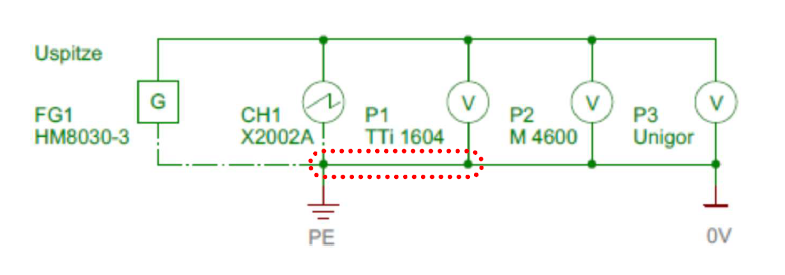
\includegraphics[width=\textwidth]{skizze_1}
		\captionof{figure}{Skizze des Schaltplans, der für die erste Aufgabe benötigt wird \cite{phasevorlage}}
		\label{fig:1}
	\end{minipage}
\end{center}

\noindent Der tatsächliche Aufbau ist in folgender \autoref{fig:aufbau1} sichtbar.

\begin{center}
	\begin{minipage}[t]{0.7\textwidth}
		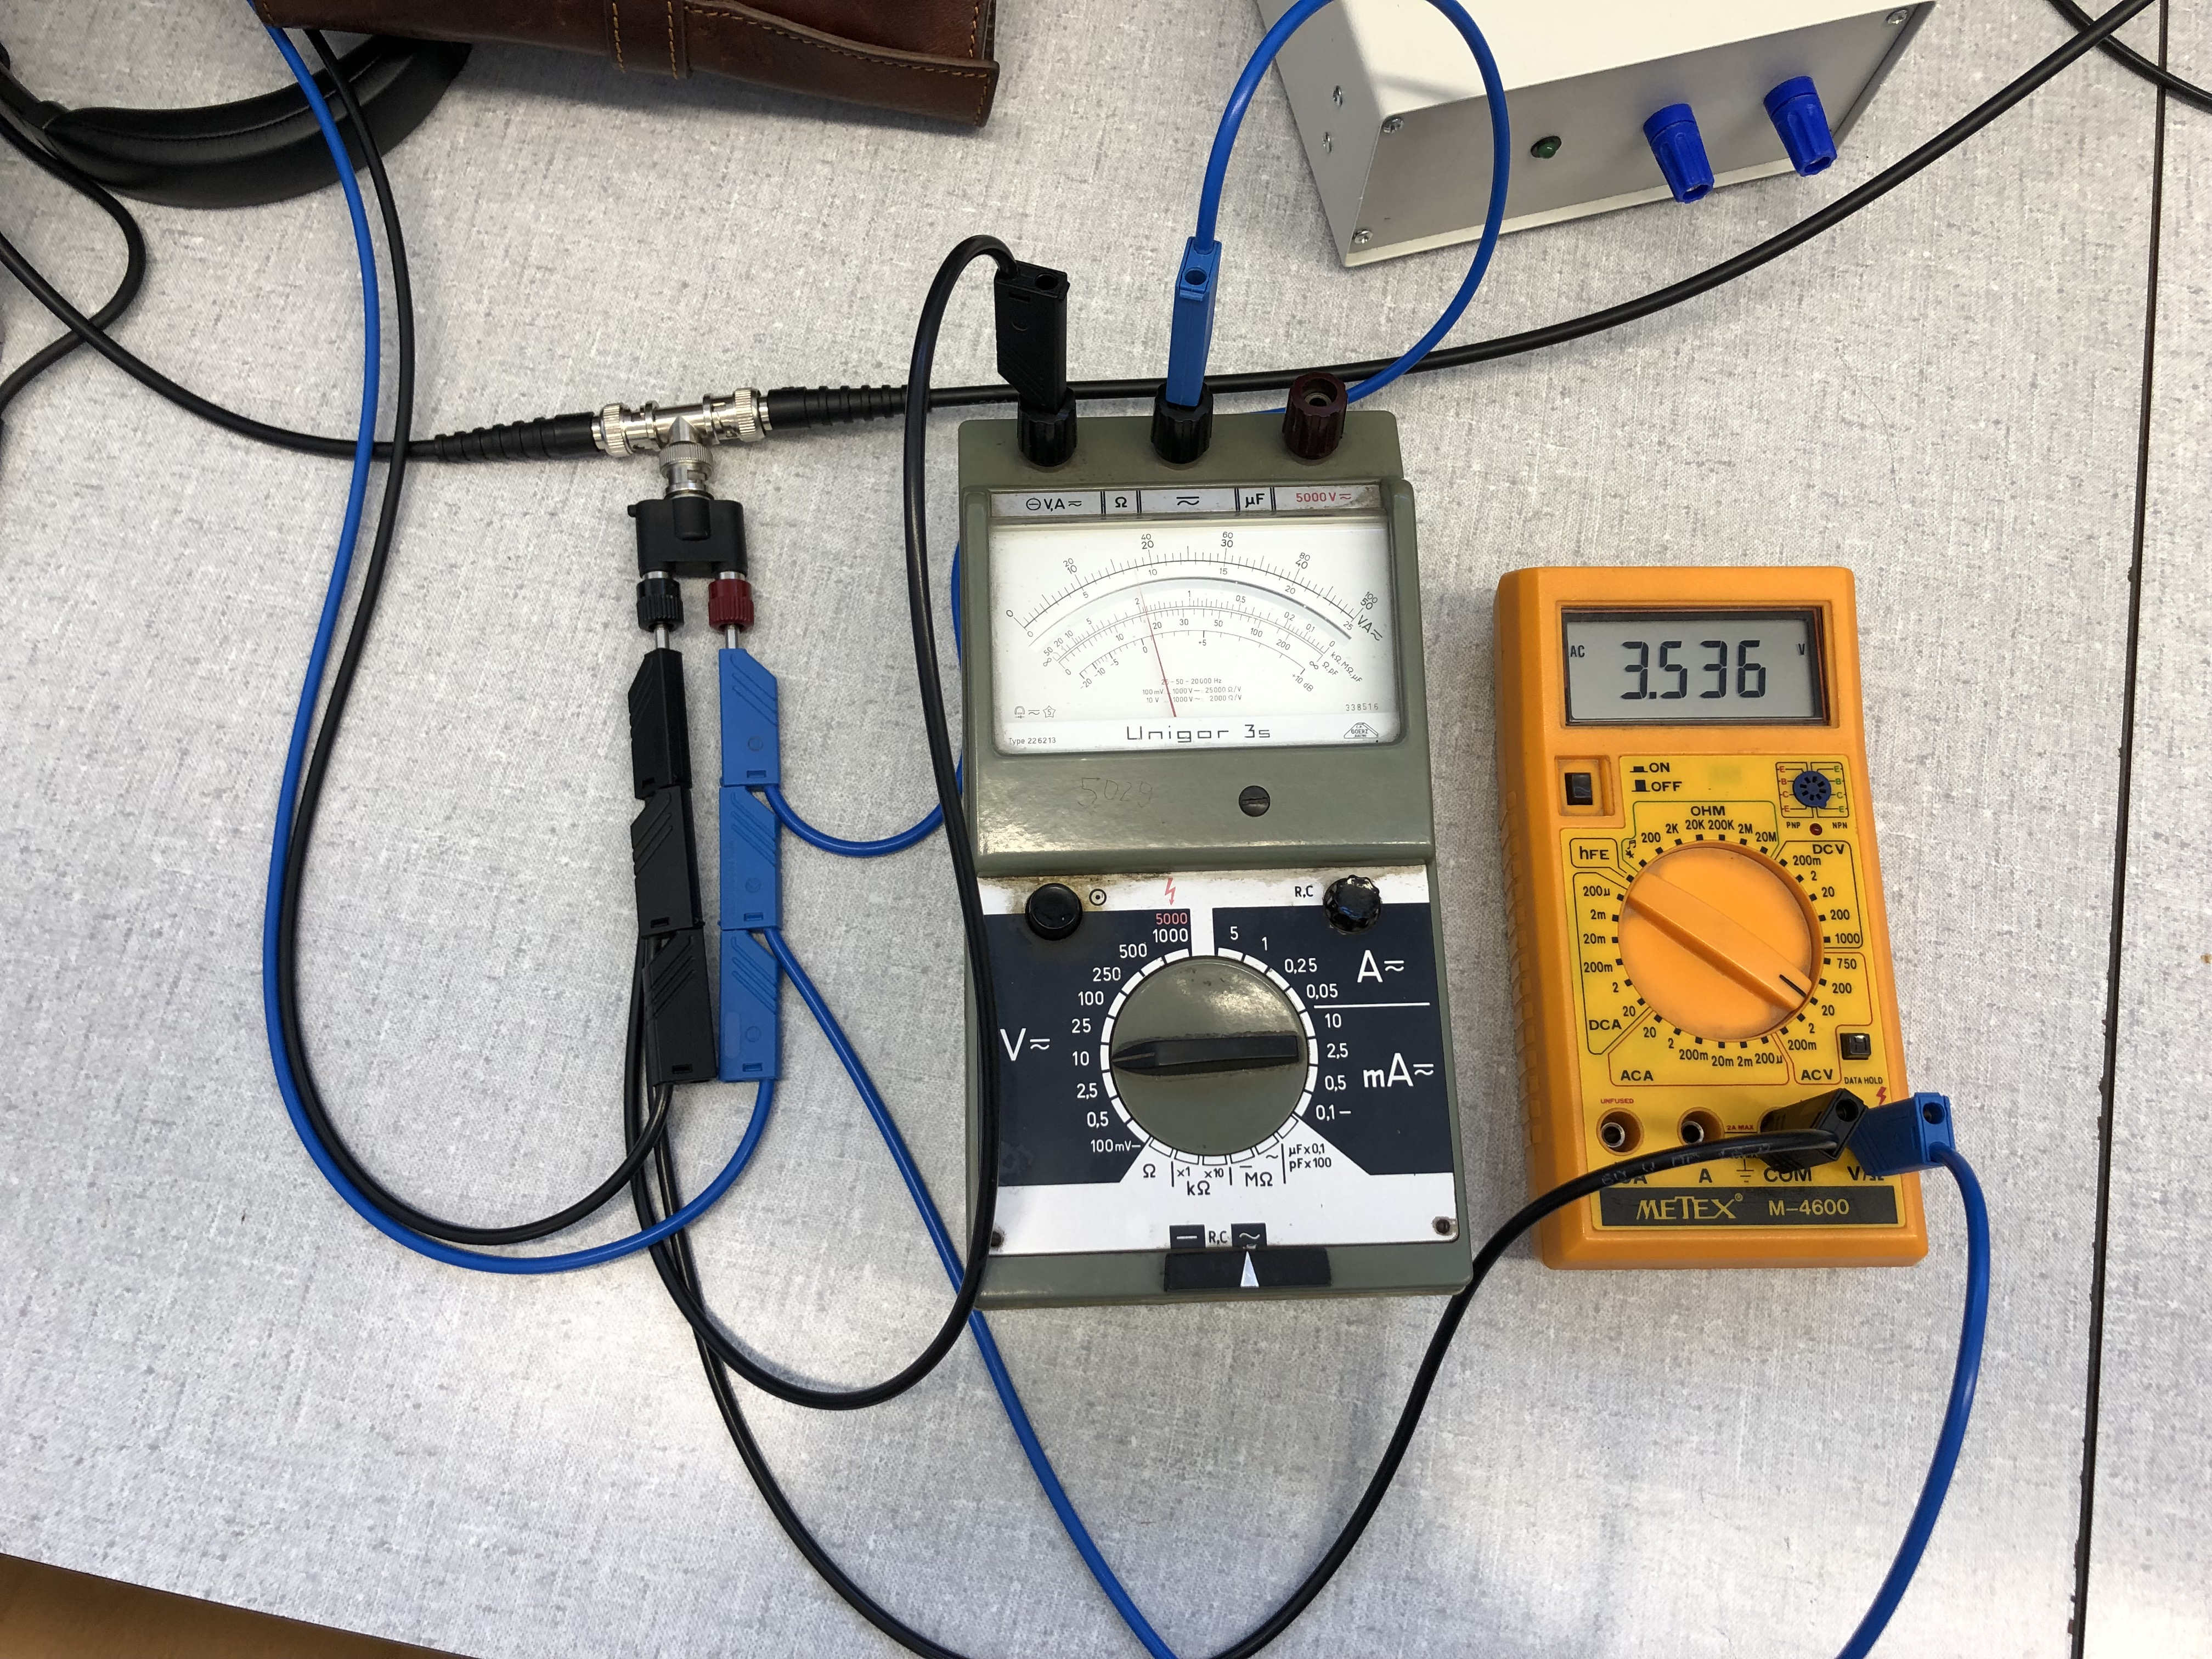
\includegraphics[width=\textwidth]{aufbau1}
		\captionof{figure}{Versuchsaufbau für die Ermittlung der Anzeige von unterschiedlichen Spannungsmessinstrumenten}
		\label{fig:aufbau1}
	\end{minipage}
\end{center}

Bei der Eingangsspannung wird dabei zwischen einer Sinus-, Dreiecks- und
Rechteckspannung variiert und die entsprechenden aufgezeichneten Spannungen an
den verschiedenen Multimeter abgelesen und in folgender Tabelle notiert. Die
Unsicherheit des analogen Multimeters ist dabei aufgrund von
Ableseungenauigkeiten so groß gewählt.  Rechnet man die Unsicherheit nach
\cite{uncertaintyoszi} aus erhält man sehr hohe Unsicherheiten. Daher wird die Unsicherheit
nach folgender Formel in \autoref{eq:du}berechnet.  LSB bezeichnet dabei die
``least significant bit`` und ergibt sich konkret als $(\frac{1}{2})^8$.

\begin{equation}
	\Delta U = 2\text{\%}\, 8\text{div}\, \text{*}\, \frac{\text{V}}{\text{div}} + 1\text{LSB}
	\label{eq:du}
\end{equation}

\begin{table}[H]
	\caption{Abgelesene Werte auf den verschiedenen Multimeter für die Spannung
		beim entsprechenden Signal, dabei sind alle Geräte ``true RMS``, bis auf
		das analoge, welches den ``true RMS`` analog misst $U_{Oszi}$ \dots
		abgelesener Wert der ``Peak to Peak`` Spannung am Oszilloskop in V,
		Unsicherheit nach \autoref{eq:du} \\ $U_{theo}$ \dots theoretisch
		ausgerechnete Spannung aus dem ``Peak to Peak`` Wert des Oszilloskops in V
		\\ $U_{TTi}$ \dots abgelesener Wert der Spannung am digitalen Multimeter
		der Marke TTi in V, Unsicherheit \cite{ttimeter} \\ $U_{Metex}$ \dots abgelesener
		Wert der Spannung am Multimeter der Marke Metex in V, Unsicherheit \cite{metex}
		\\ $U_{Unigor}$ \dots abgelesener Wert der Spannung am analogen Multimeter
		der Marke Unigor in V, Unsicherheit \cite{unigor} }
	\begin{center}
		\begin{tabular}{|c|c|c|c|c|c|} \hline
			\textbf{Spannungsart} & $U_{Oszi}$ / V & $U_{theo}$ / V   & $U_{TTi}$ / V    & $U_{Metex}$ / V & $U_{Unigor}$ / V \\ \hline
			Sinusspannung         & \SI{8.06(4)}{} & \SI{2.849(14)}{} & \SI{2.986(19)}{} & \SI{2.98(3)}{}  & \SI{2.9(1)}{}    \\
			Dreieckspannung       & \SI{8.46(4)}{} & \SI{2.327(12)}{} & \SI{2.447(17)}{} & \SI{2.36(3)}{}  & \SI{2.20(5)}{}   \\
			Rechteckspannung      & \SI{8.05(4)}{} & \SI{4.03(2)}{}   & \SI{4.03(6)}{}   & \SI{4.19(4)}{}  & \SI{4.2(1)}{}    \\ \hline
		\end{tabular}
		\label{tab:1b}
	\end{center}
\end{table}


\newpage

\subsection{Phasenlage von Strom und Spannung an einem Kondensator}

Nun wird der Stromkreis nach folgenden Schaltplan in \autoref{fig:2} aufgebaut, um den Strom und die Spannung am Kondensator mithilfe des Oszilloskops gemessen. Dabei werden 2 verschiedene Kondensatoren verwendet. Wie bereits erwähnt wurde das Oszilloskop mithilfe von Tastkabeln in den Stromkreis geschlossen, weil diese besser an das Gerät angepasst sind.

\begin{center}
	\begin{minipage}[t]{0.5\textwidth}
		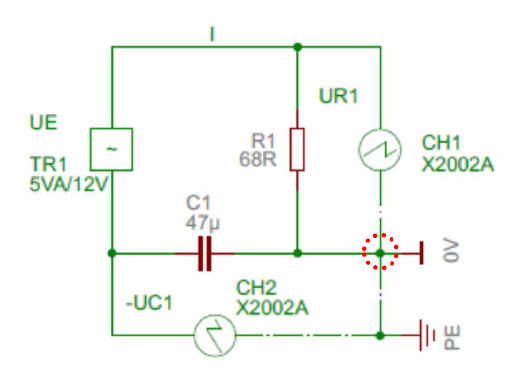
\includegraphics[width=\textwidth]{skizze_2}
		\captionof{figure}{Skizze des Schaltplans, der für die Messung der
			Phasenlage von Strom und Spannung an einem Kondensator benötigt wird
			\cite{phasevorlage}}
		\label{fig:2}
	\end{minipage}
\end{center}

\noindent Der tatsächliche Aufbau ist in folgender \autoref{fig:aufbau2} sichtbar.

\begin{center}
	\begin{minipage}[t]{0.7\textwidth}
		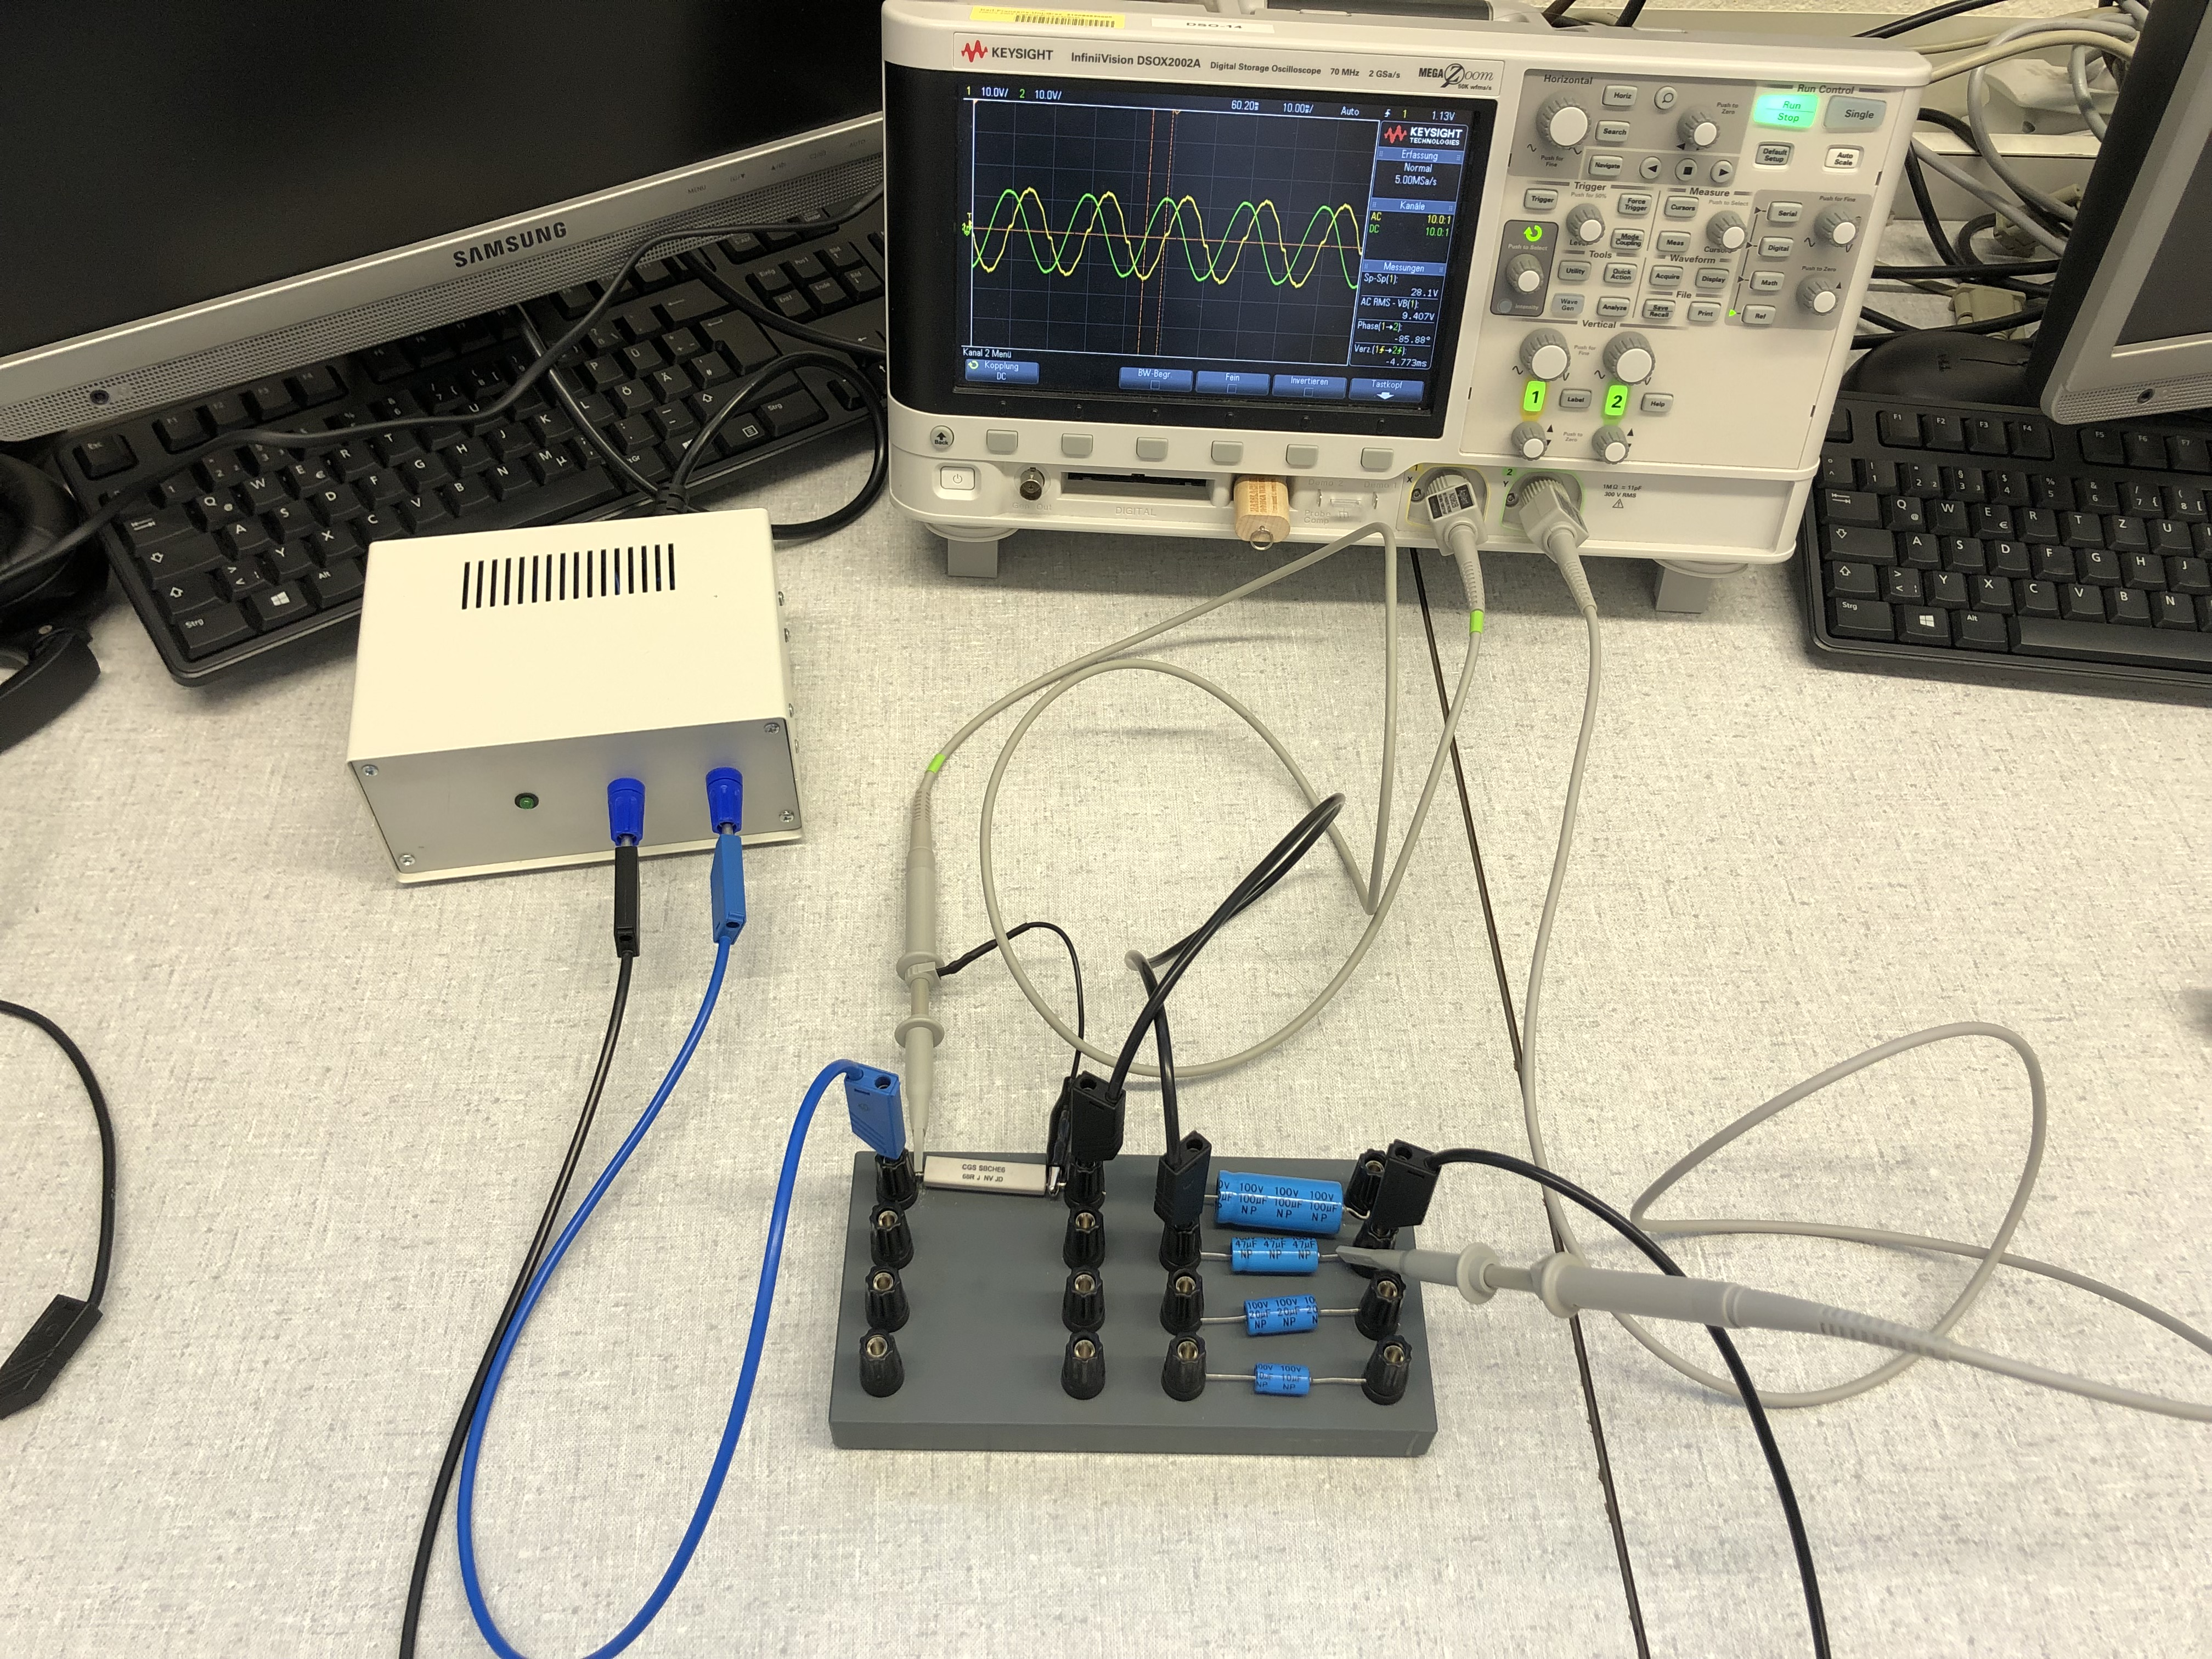
\includegraphics[width=\textwidth]{aufbau2}
		\captionof{figure}{Versuchsaufbau für die Messung der Phasenlage von Strom und Spannung an einem Kondensator}
		\label{fig:aufbau2}
	\end{minipage}
\end{center}

Die vom Oszilloskop aufgezeichneten Signale sind in folgenden Abbildungen sichtbar. Zusätzlich wurden diese mithilfe eines USB Sticks als CSV Datei für die spätere Auswertung gespeichert.

\begin{minipage}{\textwidth}
	\begin{minipage}[t]{0.5\textwidth}
		\centering
		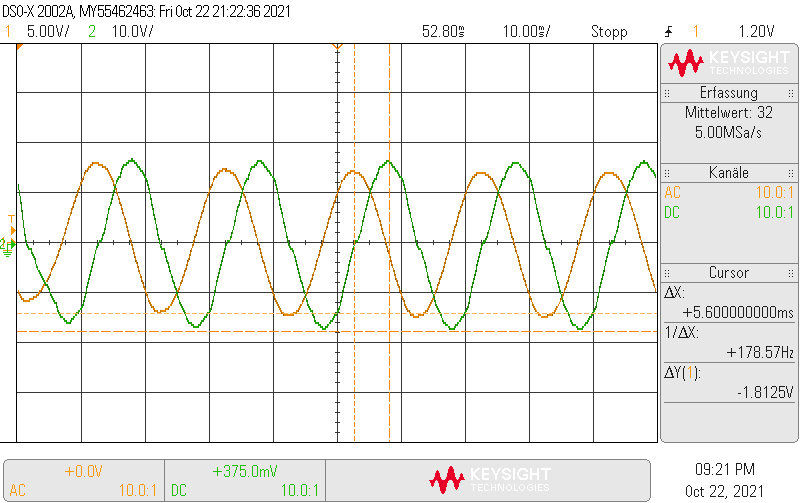
\includegraphics[width=\textwidth]{Phasenzeug/scope_1}
		\captionbelowof{figure}{Vom Oszilloskop aufgezeichnetes Signal mit der Verwendung des Kondensators mit einer Kapazität von 100 $\mu$ Farad}
		\label{fig:oszi1_100}
	\end{minipage}
	\vspace{2mm}
	\begin{minipage}[t]{0.5\textwidth}
		\centering
		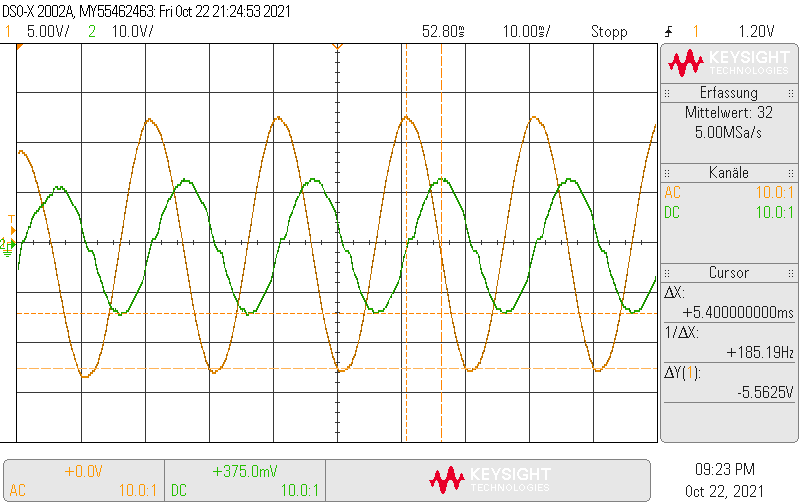
\includegraphics[width=\textwidth]{Phasenzeug/scope_2}
		\captionof{figure}{Vom Oszilloskop aufgezeichnetes Signal mit der Verwendung des Kondensators mit einer Kapazität von 70 $\mu$ Farad}
		\label{fig:oszi1_70}
	\end{minipage}
	\vspace{1em}
\end{minipage}


\subsection{Phasenlage von Strom und Spannung an einer Spule}

Zunächst wird der Stromkreis nach folgenden Schaltplan in \autoref{fig:3} aufgebaut. Das Oszilloskop wird wie bereits zuvor erklärt mithilfe der Tastkabel in die Schaltung integriert.

\begin{center}
	\begin{minipage}[t]{0.5\textwidth}
		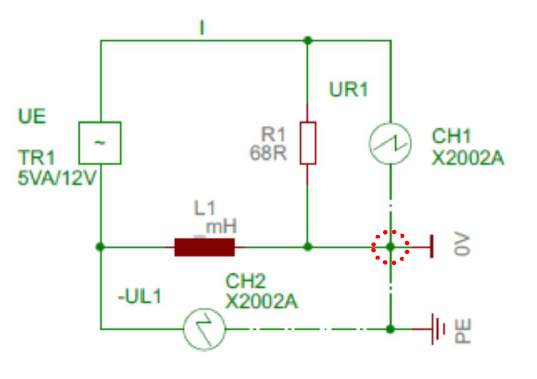
\includegraphics[width=\textwidth]{skizze_3}
		\captionof{figure}{Skizze des Schaltplans, der für die Messung der
			Phasenlage von Strom und Spannung an einer Spule benötigt wird
			\cite{phasevorlage}}
		\label{fig:3}
	\end{minipage}
\end{center}

\noindent Der tatsächliche Aufbau ist in folgender \autoref{fig:aufbau3} sichtbar.

\begin{center}
	\begin{minipage}[t]{0.7\textwidth}
		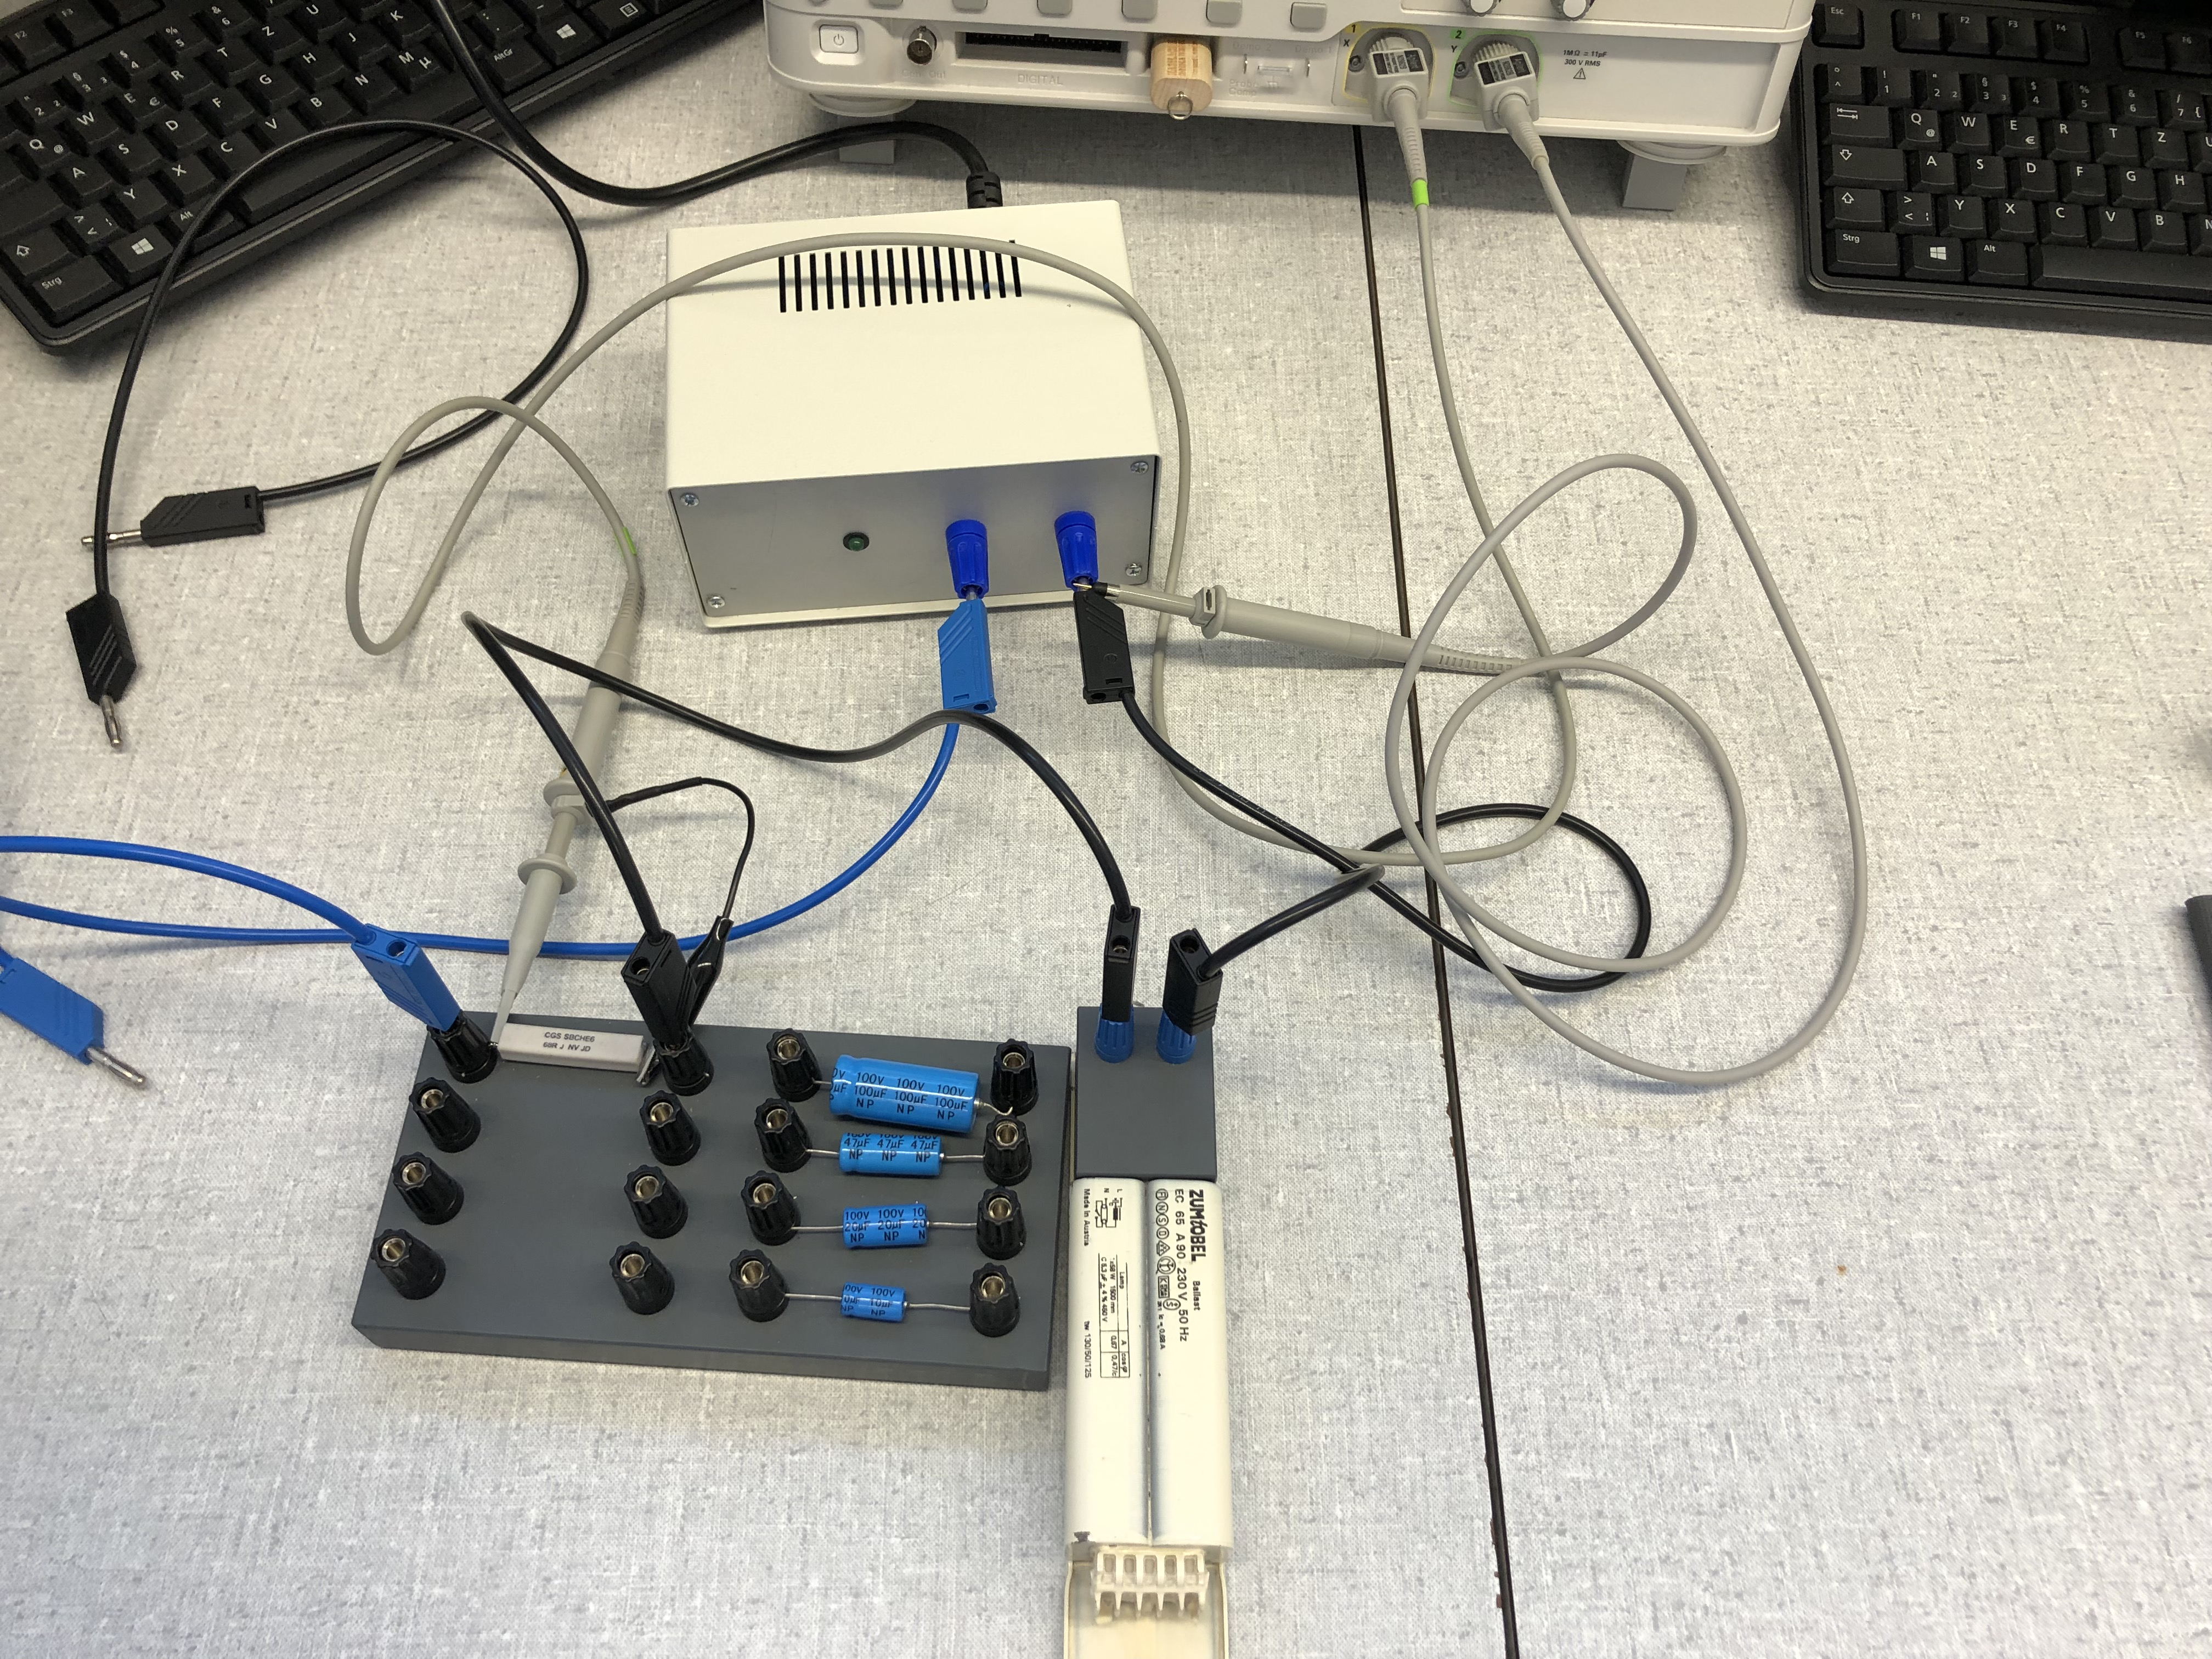
\includegraphics[width=\textwidth]{aufbau3}
		\captionof{figure}{Versuchsaufbau für die Messung der Phasenlage von Strom und Spannung an einer Spule}
		\label{fig:aufbau3}
	\end{minipage}
\end{center}

Das vom Oszilloskop aufgezeichnete Signal ist in folgender \autoref{fig:oszi_2} sichtbar. Auch die entsprechenden CSV Daten wurden, wie bereits erwähnt auf den USB Stick importiert.

\begin{center}
	\begin{minipage}[t]{0.7\textwidth}
		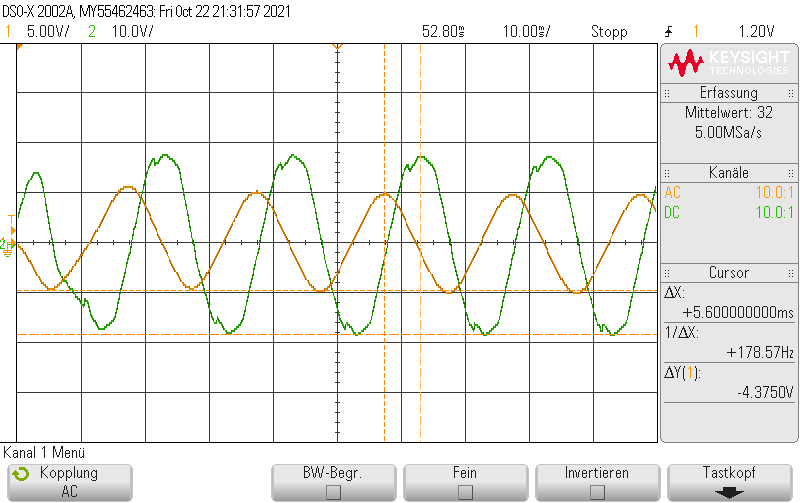
\includegraphics[width=\textwidth]{Phasenzeug/scope_5}
		\captionof{figure}{Vom Oszilloskop aufgezeichnetes Signal mit der Verwendung der Spule}
		\label{fig:oszi_2}
	\end{minipage}
\end{center}

Um den Phasenwinkel zwischen den beiden Kurven leichter bestimmen zu können, wurde dieser mithilfe des Oszilloskops bestimmt, was in folgender \autoref{fig:oszi_2_winkel} sichtbar ist.

\begin{center}
	\begin{minipage}[t]{0.7\textwidth}
		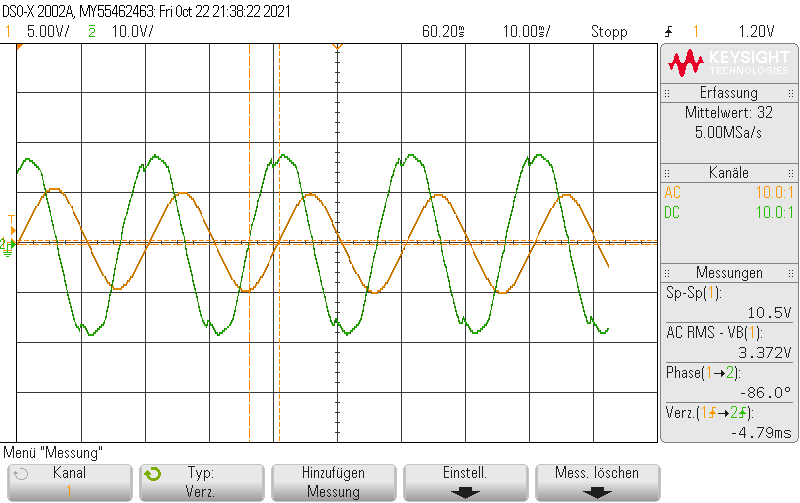
\includegraphics[width=\textwidth]{Phasenzeug/scope_6}
		\captionof{figure}{Vom Oszilloskop aufgezeichnetes Signal mit der Verwendung der Spule, bei der der Phasenwinkel angezeigt wird}
		\label{fig:oszi_2_winkel}
	\end{minipage}
\end{center}





\subsection{elektrische Leistung in einer RC-Schaltung}

Nun wird der Stromkreis nach folgenden Schaltplan in \autoref{fig:4} aufgebaut. Weil es sich beim ``Power Supply`` um den ``HM8115-2`` Typ handelt kann der einfachere linke Aufbau verwendet werden.

\begin{center}
	\begin{minipage}[t]{0.8\textwidth}
		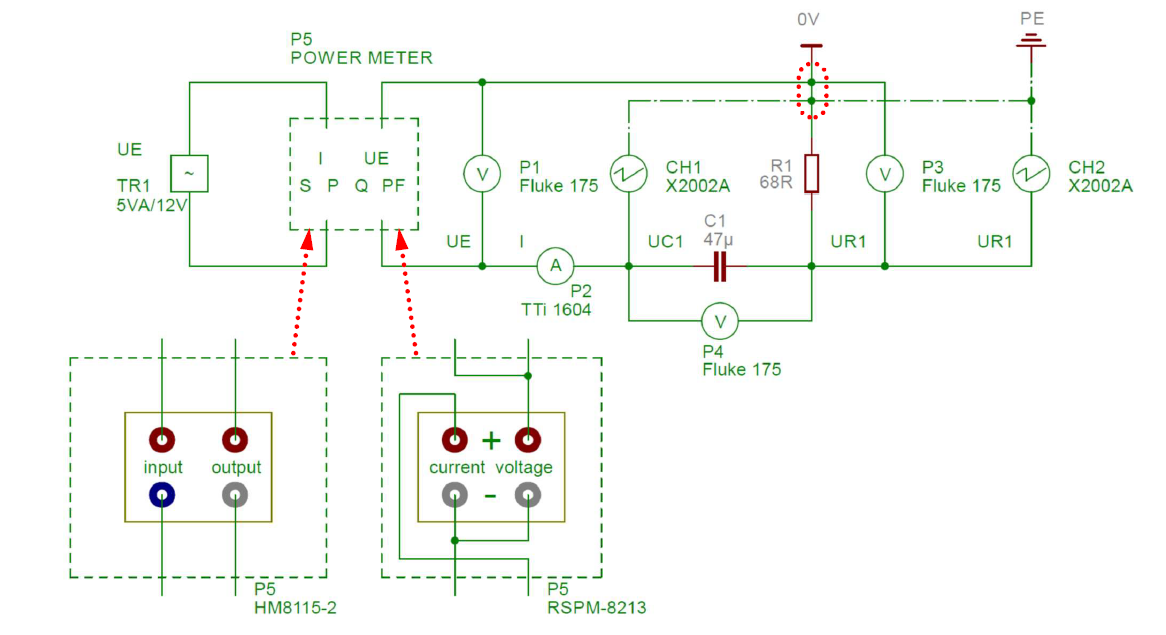
\includegraphics[width=\textwidth]{skizze_4}
		\captionof{figure}{Skizze des Schaltplans für die RC Schaltung \cite{phasevorlage}}
		\label{fig:4}
	\end{minipage}
\end{center}

\noindent Der tatsächliche Aufbau ist in folgender \autoref{fig:aufbau4} sichtbar.

\begin{center}
	\begin{minipage}[t]{0.7\textwidth}
		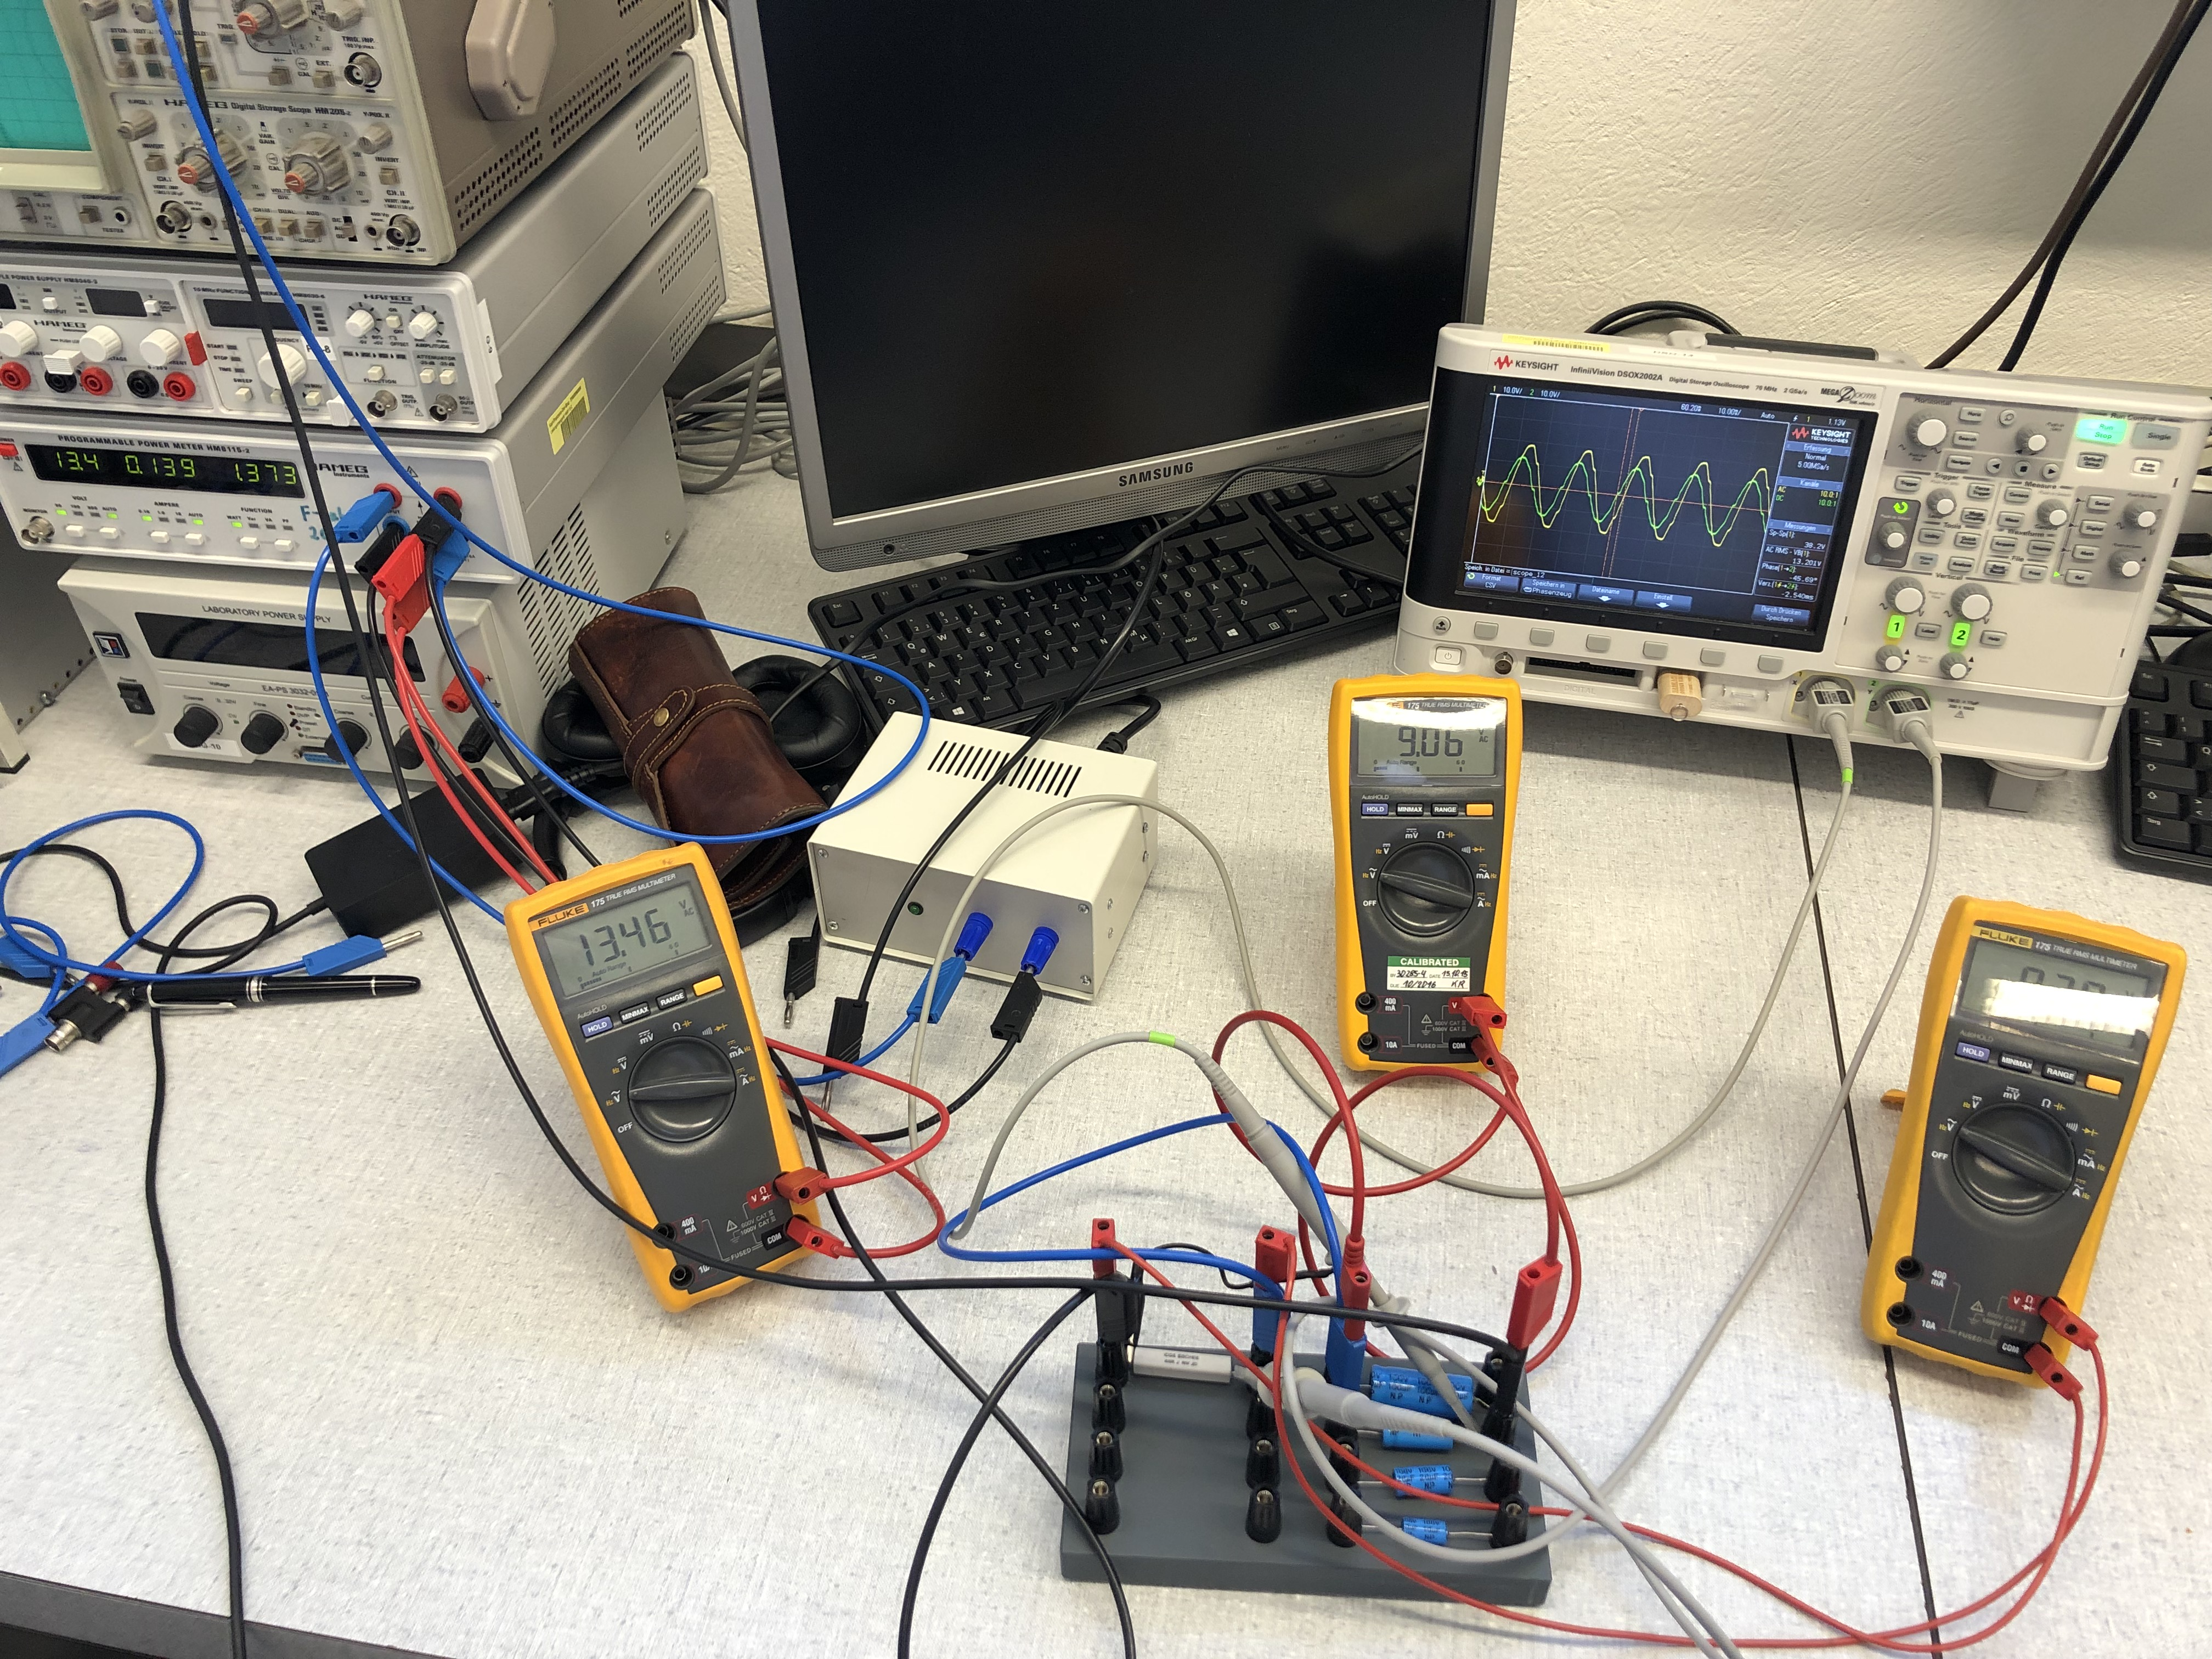
\includegraphics[width=\textwidth]{aufbau4}
		\captionof{figure}{Versuchsaufbau für die RC Schaltung}
		\label{fig:aufbau4}
	\end{minipage}
\end{center}

Das vom Oszilloskop aufgezeichnete Signal ist in folgender \autoref{fig:oszi_4} ersichtlich. Mit der entsprechenden Einstellung wird auch hier wieder direkt der Phasenwinkel eingeblendet, der im konkreten Fall 45.92° beträgt.

\begin{center}
	\begin{minipage}[t]{0.7\textwidth}
		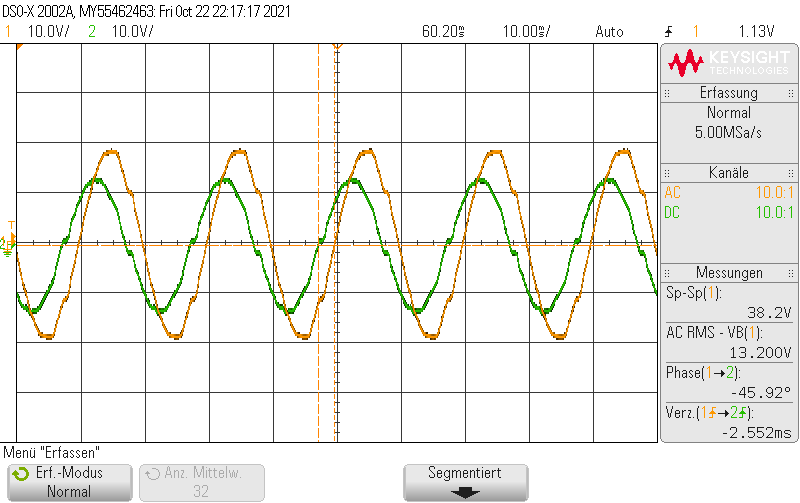
\includegraphics[width=\textwidth]{Phasenzeug/scope_13}
		\captionof{figure}{Vom Oszilloskop aufgezeichnetes Signal bei einer RC Schaltung}
		\label{fig:oszi_4}
	\end{minipage}
\end{center}

Zusätzlich werden von den Messgeräten folgende Daten, siehe \autoref{tab:4}, abgelesen. Die Daten am ``Power Supply`` können dabei durch Drücken der jeweiligen Knöpfe angezeigt werden.

\begin{table}[H]
	\captionof{table}{Abgelesene Werte auf den verschiedenen Geräten bei der RC
		Schaltung \\ $U_{C}$ \dots abgelesener Wert der Spannung am Kondensator in
		V, Unsicherheit \cite{fluke} \\ $U_{R}$ \dots abgelesener Wert der Spannung
		am Widerstand in V, Unsicherheit \cite{fluke} \\ $U_{Pow}$ \dots
		abgelesener Wert der Spannung am ``Power Supply`` in V, Unsicherheit
		\cite{fluke} \\ $I$ \dots abgelesener Wert des Stroms in A, Unsicherheit
		\cite{ttimeter} \\ $U_{H}$ \dots abgelesener Wert der Spannung am ``Power
		Supply`` in V, Unsicherheit \cite{hameg} \\ $I_{H}$ \dots abgelesener Wert
		des Stroms am ``Power Supply`` in mA, Unsicherheit \cite{hameg} \\ $Va_{H}$
		\dots abgelesener Wert am ``Power Supply`` für die Scheinleistung,
		Unsicherheit \cite{hameg} \\ $Var_{H}$ \dots abgelesener Wert am ``Power
		Supply`` für die Blindleistung, Unsicherheit \cite{hameg}\\ $PF_{H}$ \dots
		abgelesener Wert am ``Power Supply``, Unsicherheit \cite{hameg}\\ $P_{H}$ \dots
		abgelesener Wert der Leistung am ``Power Supply`` in Watt, Unsicherheit
		\cite{hameg}}
	\begin{center}
		\begin{tabular}{|c|c|c|} \hline
			{}               & \textbf{Typ} & \textbf{Wert}       \\ \hline
			Voltmeter        & $U_{C}$      & \SI{9.05(13)}{\V}   \\
			                 & $U_{R}$      & \SI{9.31(13)}{\V}   \\
			                 & $U_{Pow}$    & \SI{13.49(17)}{\V}  \\ \hline
			Amperemeter      & $I$          & \SI{140(5)}{\mA}    \\ \hline
			``Power Supply`` & $U_{H}$      & \SI{13.4(6)}{\V}    \\
			                 & $I_{H}$      & \SI{0.139(6)}{\A}   \\
			                 & $Va_{H}$     & \SI{1.851(19)}{Va}  \\
			                 & $Var_{H}$    & \SI{1.24(16)}{Var}  \\
			                 & $PF_{H}$     & \SI{0.74(5)}{}      \\
			                 & $P_{H}$      & \SI{1.38(3)}{\watt} \\ \hline
		\end{tabular}
		\label{tab:4}
	\end{center}
\end{table}


\subsection{elektrische Leistung in einer RL-Schaltung}

Zunächst wird der Stromkreis nach folgenden Schaltplan in \autoref{fig:5} aufgebaut. Wie bereits zuvor erwähnt wird dabei der linke Aufbau des Typs ``HM8115-2`` verwendet.

\begin{center}
	\begin{minipage}[t]{0.8\textwidth}
		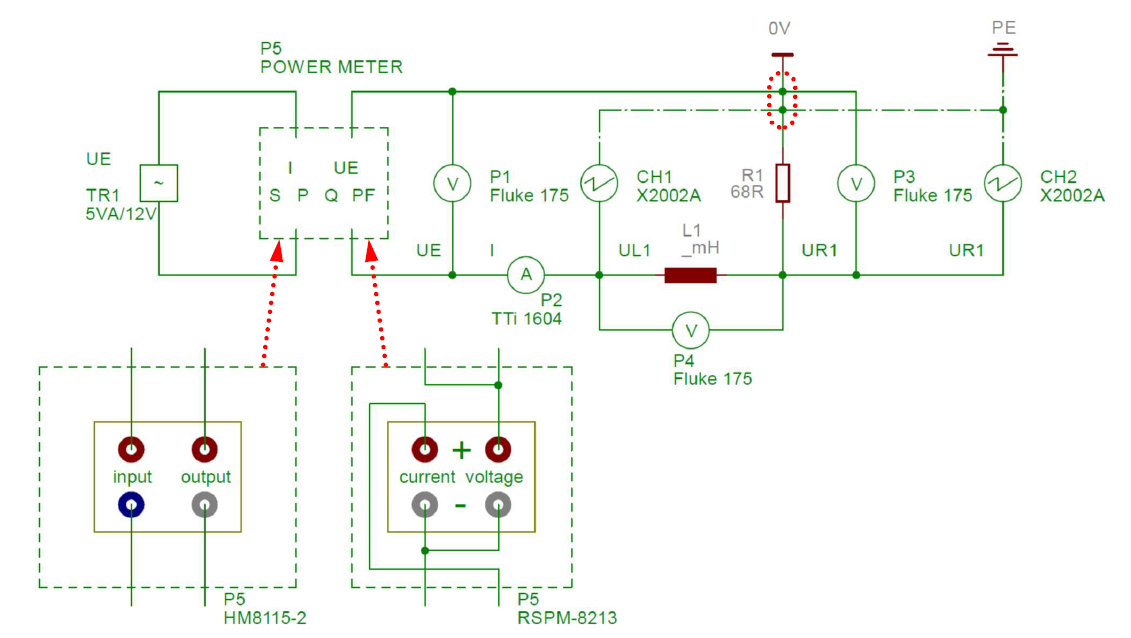
\includegraphics[width=\textwidth]{skizze_5}
		\captionof{figure}{Skizze des Schaltplans für die RL Schaltung \cite{phasevorlage}}
		\label{fig:5}
	\end{minipage}
\end{center}

\noindent Der tatsächliche Aufbau ist in folgender \autoref{fig:aufbau5} sichtbar.

\begin{center}
	\begin{minipage}[t]{0.7\textwidth}
		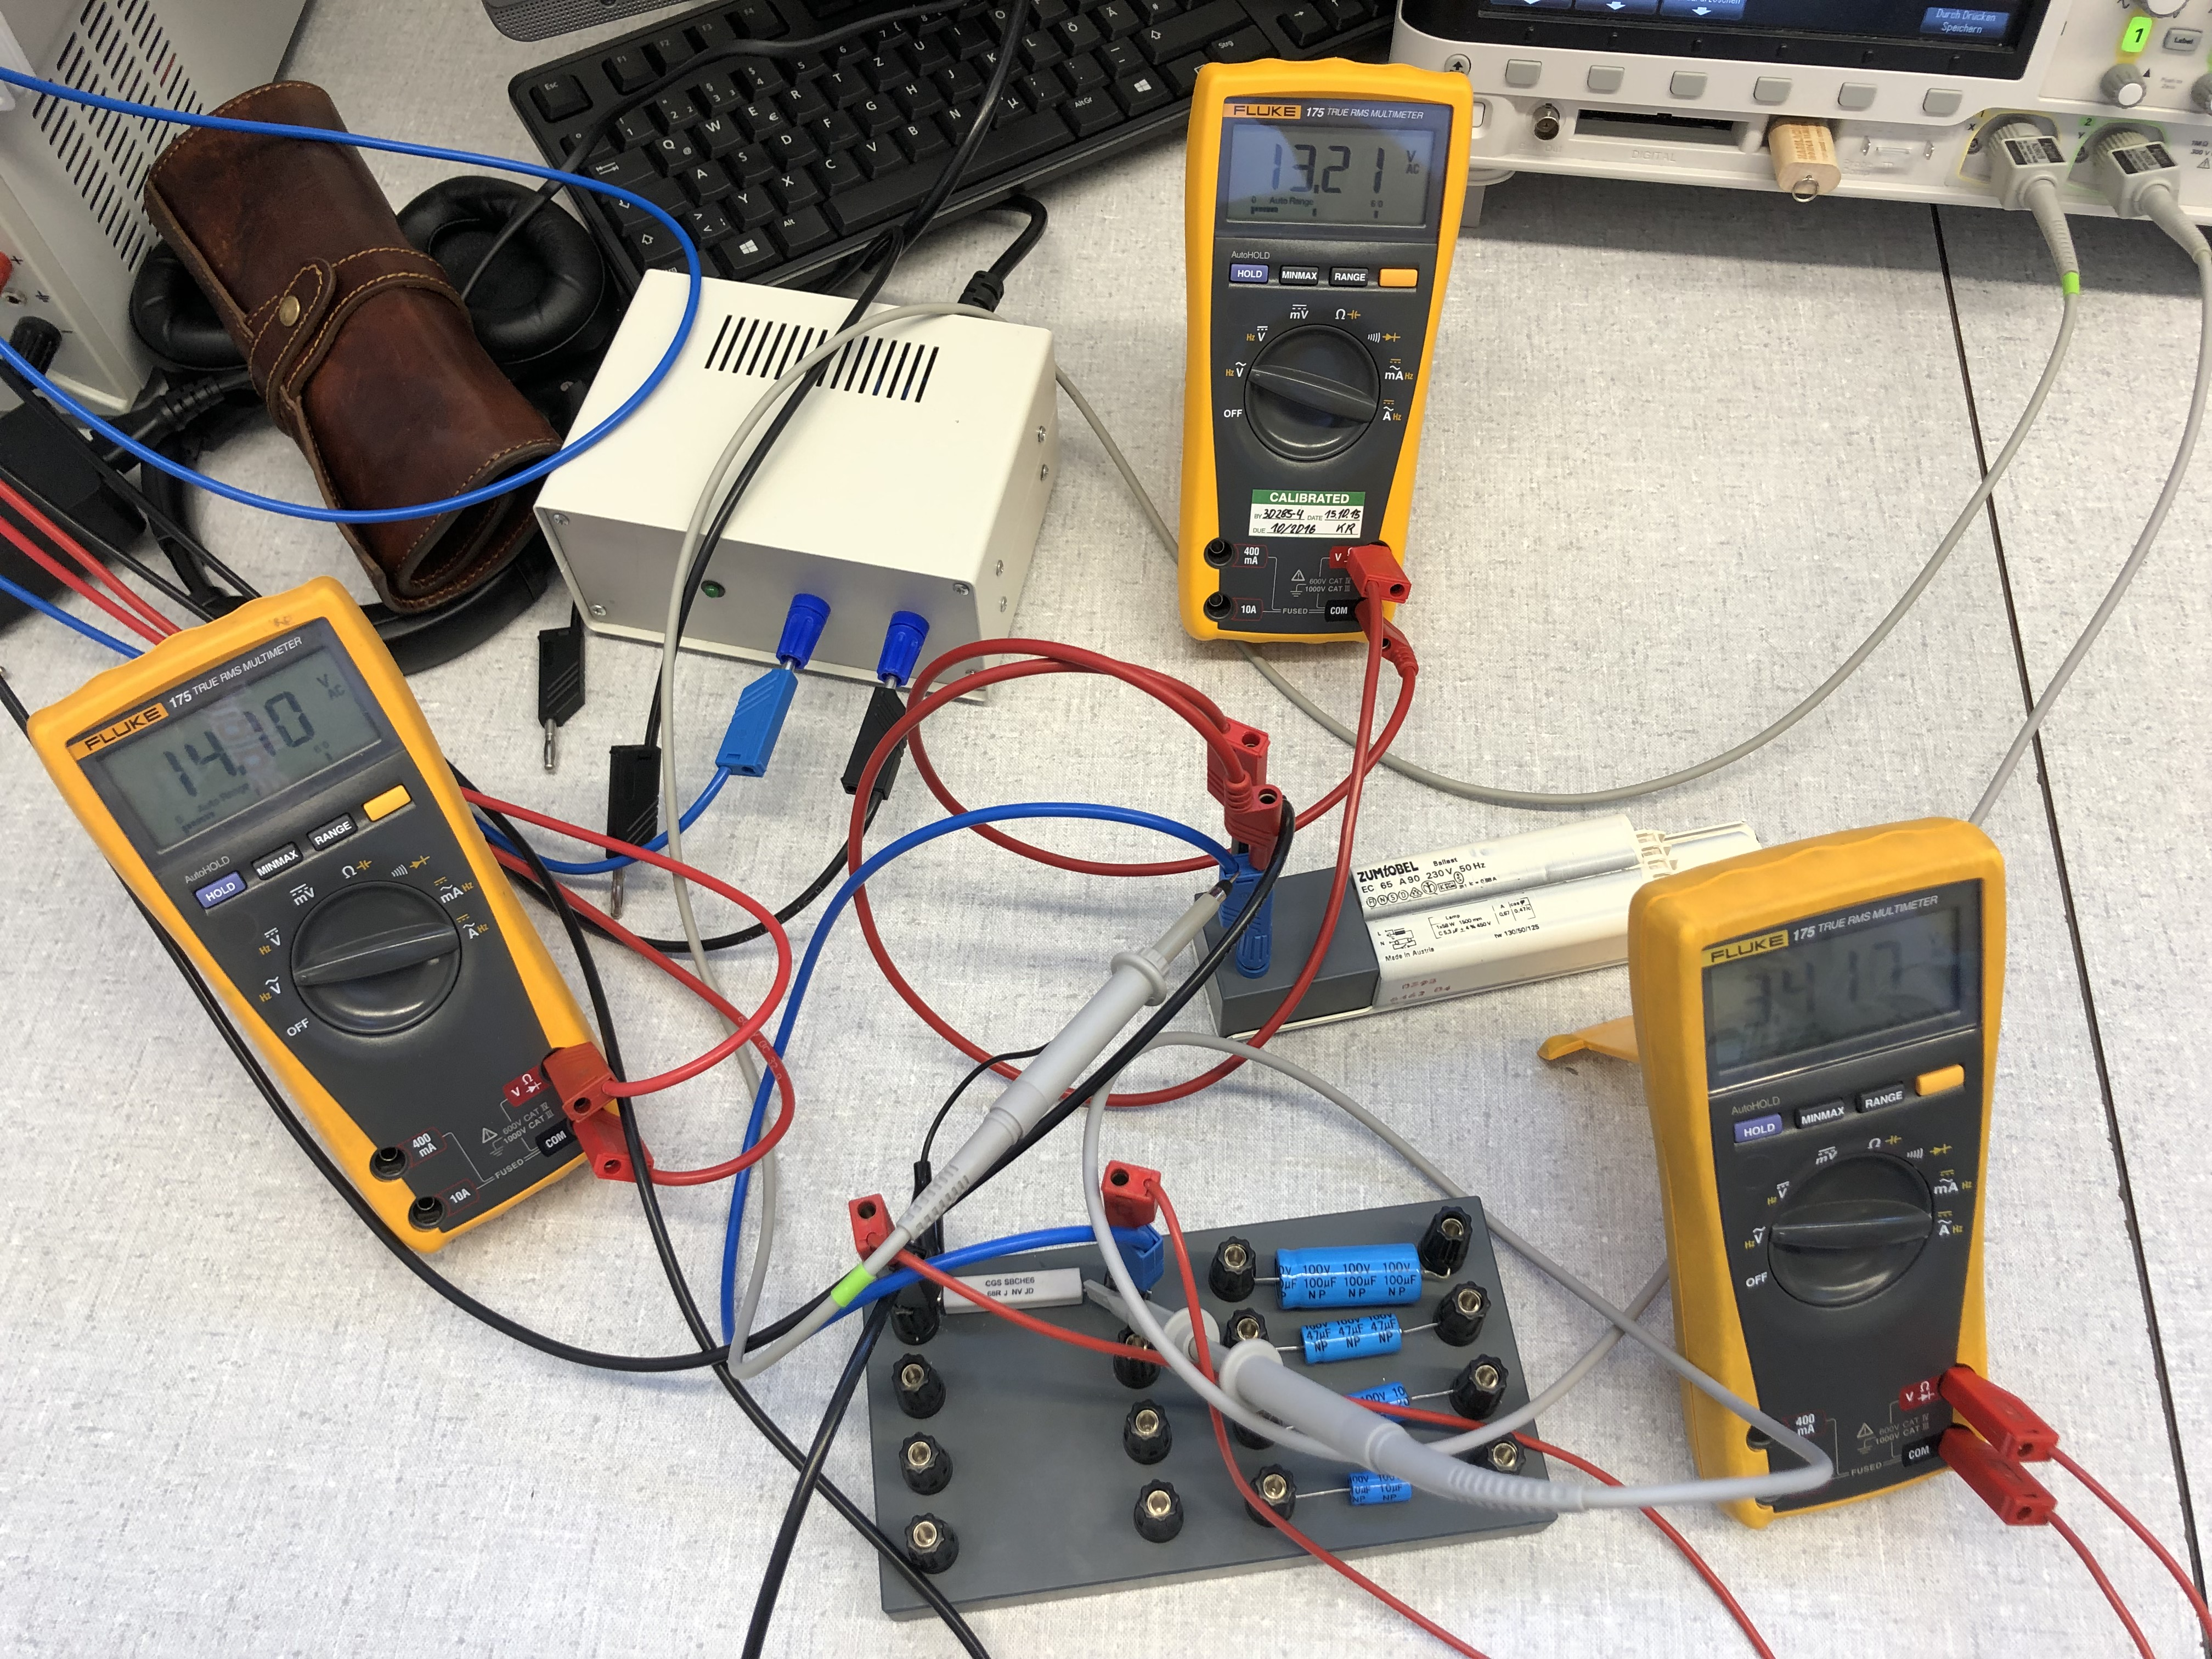
\includegraphics[width=\textwidth]{aufbau5}
		\captionof{figure}{Versuchsaufbau für die RL Schaltung}
		\label{fig:aufbau5}
	\end{minipage}
\end{center}

Das vom Oszilloskop aufgezeichnete Signal ist in folgender \autoref{fig:oszi_5} ersichtlich. Mit der entsprechenden Einstellung wird auch hier wieder direkt der Phasenwinkel eingeblendet, der im konkreten Fall 72.54° beträgt.

\begin{center}
	\begin{minipage}[t]{0.7\textwidth}
		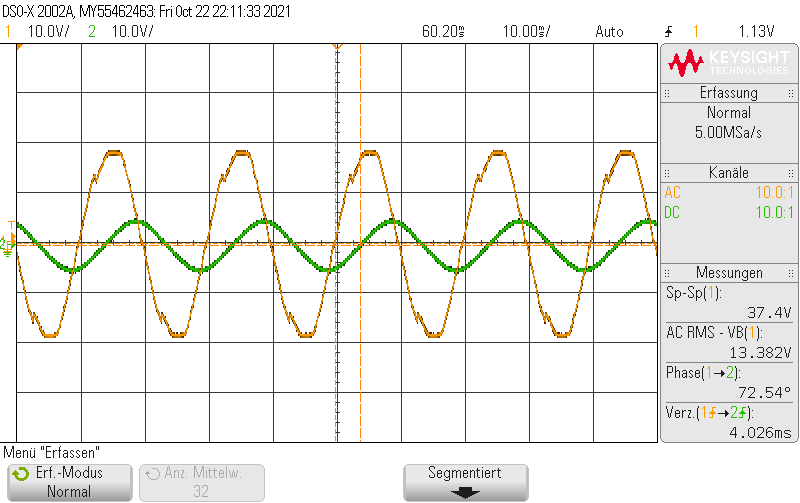
\includegraphics[width=\textwidth]{Phasenzeug/scope_10}
		\captionof{figure}{Vom Oszilloskop aufgezeichnetes Signal bei einer RL Schaltung}
		\label{fig:oszi_5}
	\end{minipage}
\end{center}

Zusätzlich werden von den Messgeräten folgende Daten, siehe \autoref{tab:5}, abgelesen. Die Daten am ``Power Supply`` können dabei durch Drücken der jeweiligen Knöpfe angezeigt werden.

\begin{table}[H]
	\captionof{table}{Abgelesene Werte auf den verschiedenen Geräten bei der RL
		Schaltung \\ $U_{L}$ \dots abgelesener Wert der Spannung an der Spule in V,
		Unsicherheit \cite{fluke} \\ $U_{R}$ \dots abgelesener Wert der Spannung am
		Widerstand in V, Unsicherheit \cite{fluke} \\ $U_{Pow}$ \dots abgelesener Wert
		der Spannung am ``Power Supply`` in V, Unsicherheit \cite{fluke} \\ $I$ \dots
		abgelesener Wert des Stroms in A, Unsicherheit \cite{ttimeter} \\ $U_{H}$ \dots
		abgelesener Wert der Spannung am ``Power Supply`` in V, Unsicherheit
		\cite{hameg} \\ $I_{H}$ \dots abgelesener Wert des Stroms am ``Power Supply`` in
		mA, Unsicherheit \cite{hameg} \\ $Va_{H}$ \dots abgelesener Wert am ``Power
		Supply`` für die Scheinleistung, Unsicherheit \cite{hameg} \\ $Var_{H}$ \dots
		abgelesener Wert am ``Power Supply`` für die Blindleistung, Unsicherheit
		\cite{hameg}\\ $PF_{H}$ \dots abgelesener Wert am ``Power Supply``, Unsicherheit
		\cite{hameg}\\ $P_{H}$ \dots abgelesener Wert der Leistung am ``Power Supply`` in
		Watt, Unsicherheit \cite{hameg}}
	\begin{center}
		\begin{tabular}{|c|c|c|} \hline
			{}               & \textbf{Typ} & \textbf{Wert}         \\ \hline
			Voltmeter        & $U_{L}$      & \SI{13.16(17)}{\V}    \\
			                 & $U_{R}$      & \SI{3.41(4)}{\V}      \\
			                 & $U_{Pow}$    & \SI{14.05(18)}{\V}    \\ \hline
			Amperemeter      & $I$          & \SI{51.5(7)}{\mA}     \\ \hline
			``Power Supply`` & $U_{H}$      & \SI{13.9(6)}{\V}      \\
			                 & $I_{H}$      & \SI{0.051(6)}{\A}     \\
			                 & $Va_{H}$     & \SI{0.715(11)}{Va}    \\
			                 & $Var_{H}$    & \SI{0.66(13)}{Var}    \\
			                 & $PF_{H}$     & \SI{0.37(4)}{}        \\
			                 & $P_{H}$      & \SI{0.262(12)}{\watt} \\ \hline
		\end{tabular}
		\label{tab:5}
	\end{center}
\end{table}




\subsection{Blindleistungskompensation eines induktiven Verbrauchers}

Zunächst wird der Stromkreis nach folgenden Schaltplan in \autoref{fig:6} aufgebaut.

\begin{center}
	\begin{minipage}[t]{0.8\textwidth}
		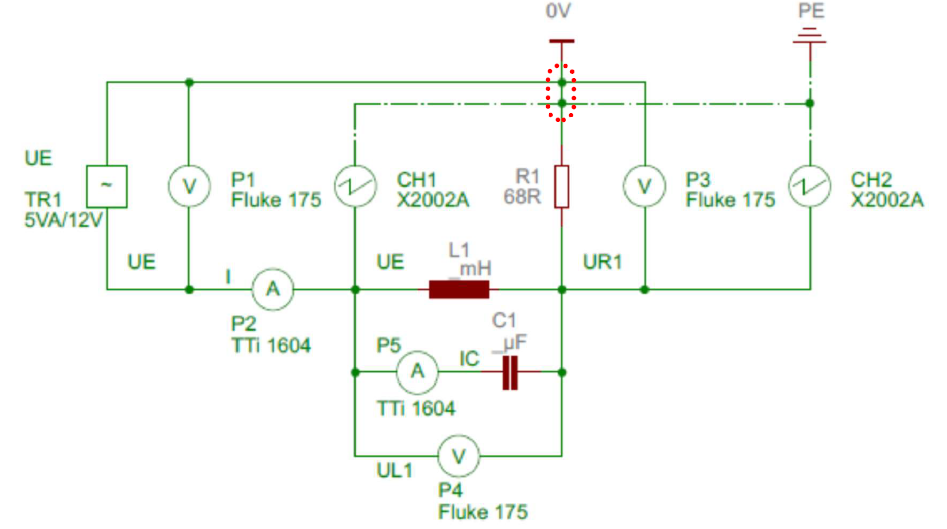
\includegraphics[width=\textwidth]{skizze_6}
		\captionof{figure}{Skizze des Schaltplans für die Bildleistungskompensation \cite{phasevorlage}}
		\label{fig:6}
	\end{minipage}
\end{center}

\newpage

Der tatsächliche Aufbau ist in folgender \autoref{fig:aufbau6} sichtbar. Das 2. Amperemeter ist dabei, der besseren Übersicht halber, nicht im Foto ersichtlich und ist an die beiden, rechts aus dem Bild ragenden, Kabel angeschlossen.

\begin{center}
	\begin{minipage}[t]{0.7\textwidth}
		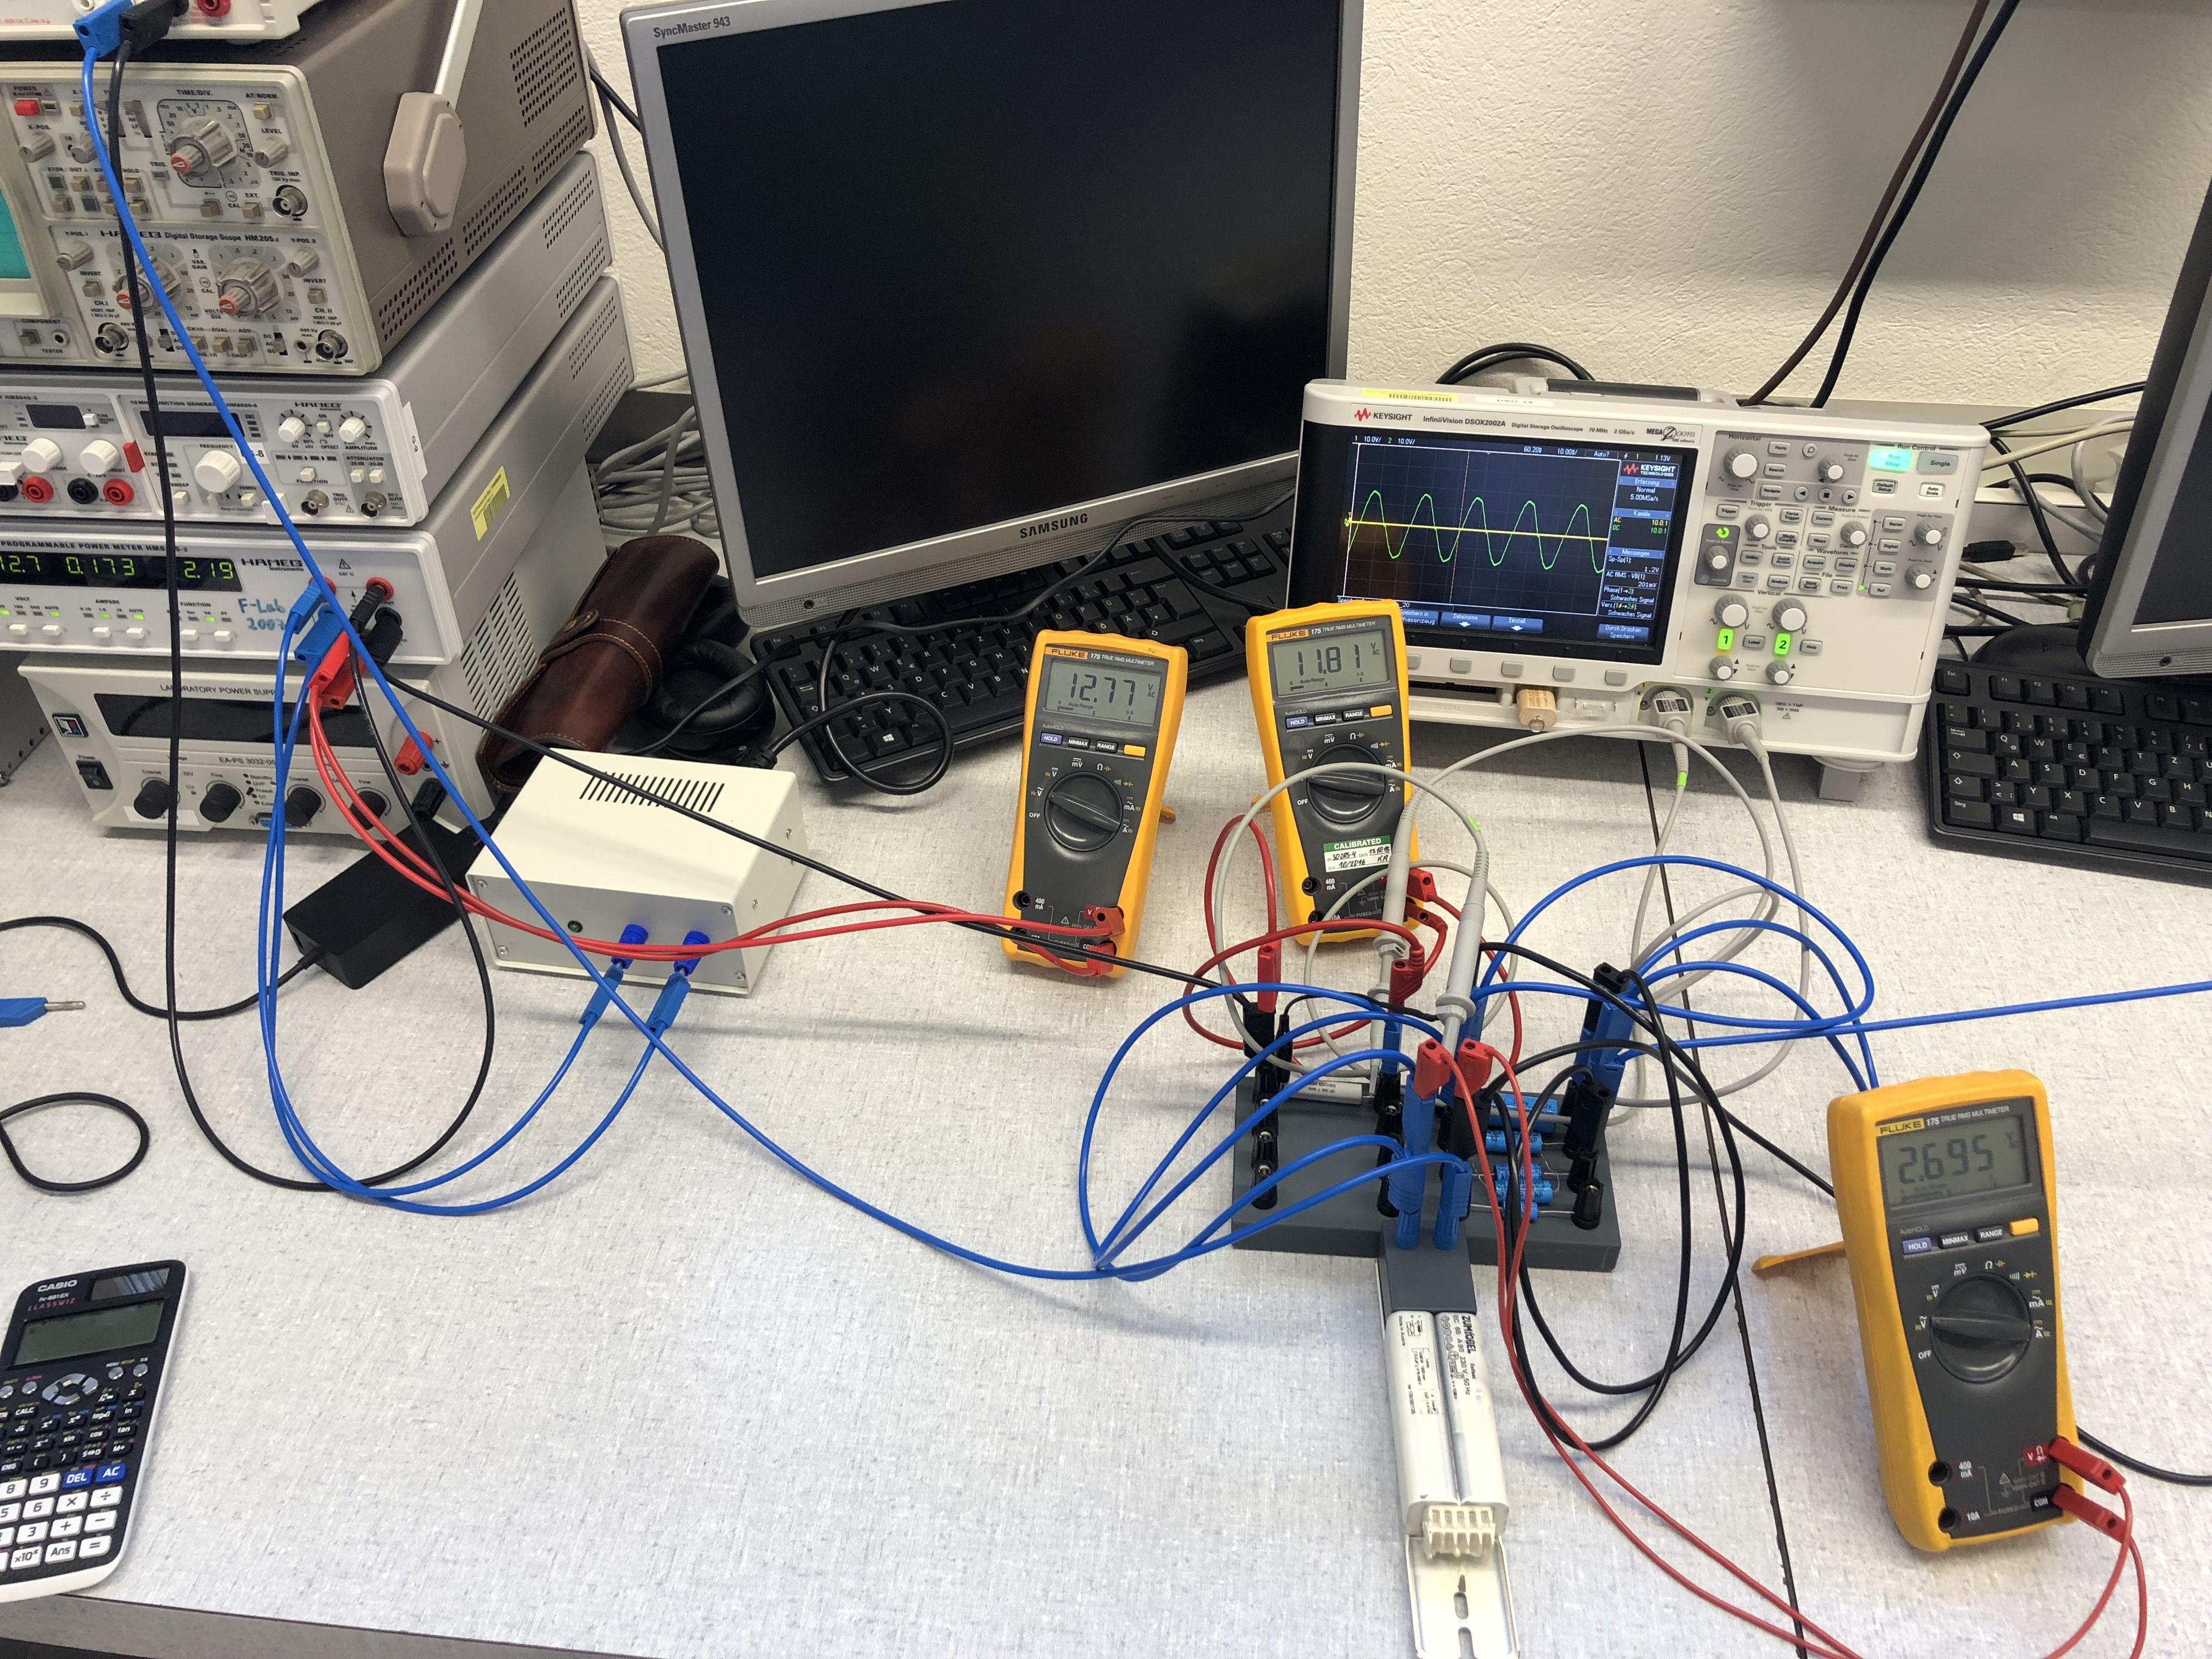
\includegraphics[width=\textwidth]{aufbau6}
		\captionof{figure}{Versuchsaufbau für die Bildleistungskompensation}
		\label{fig:aufbau6}
	\end{minipage}
\end{center}

Zunächst wurde der Kondensator mit einer Kapazität von 47 $\mu$ Farad in den Stromkreis geschlossen, was folgendes Signal aus \autoref{fig:oszi_6_47} am Oszilloskop liefert.

\begin{center}
	\begin{minipage}[t]{0.7\textwidth}
		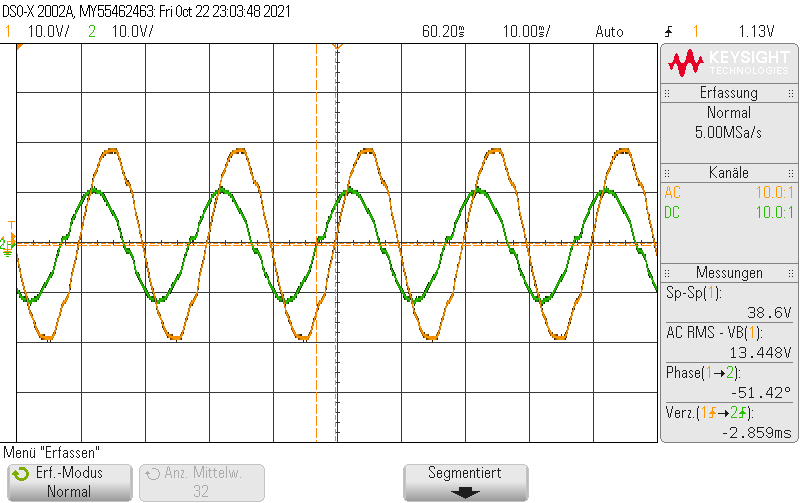
\includegraphics[width=\textwidth]{Phasenzeug/scope_14}
		\captionof{figure}{Vom Oszilloskop aufgezeichnetes Signal bei einem Kondensator mit einer Kapazität von 47 $\mu$ Farad}
		\label{fig:oszi_6_47}
	\end{minipage}
\end{center}

Die abgelesenen Daten der Messgeräte sind in folgender \autoref{tab:6_47} sichtbar.

\begin{table}[H]
	\captionof{table}{Abgelesene Werte bei Verwendung des Kondensators mit einer
		Kapazität von 47 $\mu$ Farad \\ $U_{L}$ \dots abgelesener Wert der Spannung
		an der Spule in V, Unsicherheit \cite{fluke} \\ $U_{R}$ \dots abgelesener Wert der
		Spannung am Widerstand in V, Unsicherheit \cite{fluke} \\ $U_{T}$ \dots abgelesener
		Wert der Spannung am Trafo in V, Unsicherheit \cite{fluke} \\ $I_{ges}$ \dots
		abgelesener Wert des gesamten Stroms in mA, Unsicherheit \cite{ttimeter} \\ $I_{C}$
		\dots abgelesener Wert des Stroms durch den Kondensator in mA, Unsicherheit
		\cite{ttimeter}}
	\begin{center}
		\begin{tabular}{|c|c|c|c|c|} \hline
			{}          & \textbf{Typ} & \textbf{Wert}      \\ \hline
			Voltmeter   & $U_{L}$      & \SI{10.10(14)}{\V} \\
			            & $U_{R}$      & \SI{7.81(11)}{\V}  \\
			            & $U_{T}$      & \SI{13.73(17)}{\V} \\ \hline
			Amperemeter & $I_{ges}$    & \SI{120(4)}{\mA}   \\
			            & $I_{C}$      & \SI{160(5)}{\mA}   \\ \hline
		\end{tabular}
		\label{tab:6_47}
	\end{center}
\end{table}


Nun wird zusätzlich zum Kondensator mit einer Kapazität von 47 $\mu$ Farad ein Kondensator mit der Kapazität von 100 $\mu$ Farad parallel in den Stromkreis geschlossen, was folgendes Signal aus \autoref{fig:oszi_6_147} am Oszilloskop liefert.

\begin{center}
	\begin{minipage}[t]{0.7\textwidth}
		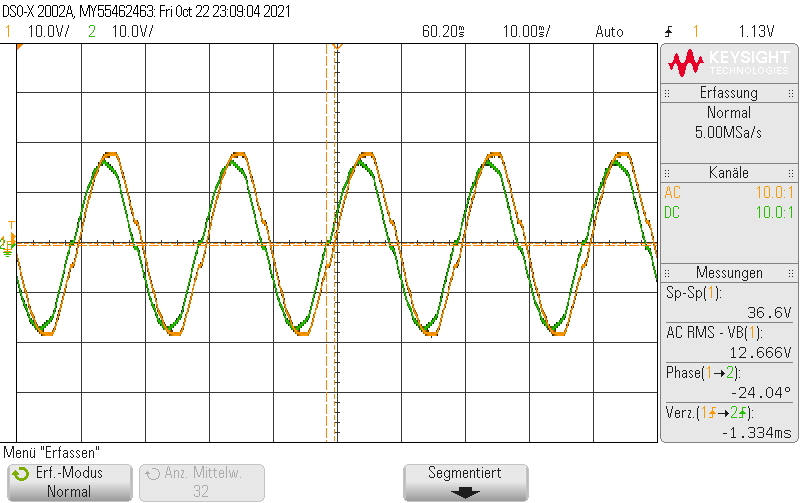
\includegraphics[width=\textwidth]{Phasenzeug/scope_18}
		\captionof{figure}{Vom Oszilloskop aufgezeichnetes Signal bei einem Kondensator mit einer gesamten Kapazität von 147 $\mu$ Farad}
		\label{fig:oszi_6_147}
	\end{minipage}
\end{center}

Die abgelesenen Daten der Messgeräte sind in folgender \autoref{tab:6_147} sichtbar.

\begin{table}[H]
	\captionof{table}{Abgelesene Werte bei Verwendung des Kondensators mit einer
		gesamten Kapazität von 147 $\mu$ Farad \\ $U_{L}$ \dots abgelesener Wert der
		Spannung an der Spule in V, Unsicherheit \cite{fluke} \\ $U_{R}$ \dots abgelesener
		Wert der Spannung am Widerstand in V, Unsicherheit \cite{fluke} \\ $U_{T}$ \dots
		abgelesener Wert der Spannung am Trafo in V, Unsicherheit \cite{fluke} \\ $I_{ges}$
		\dots abgelesener Wert des gesamten Stroms in mA, Unsicherheit \cite{ttimeter} \\
		$I_{C}$ \dots abgelesener Wert des Stroms durch den Kondensator in mA,
		Unsicherheit \cite{ttimeter}}
	\begin{center}
		\begin{tabular}{|c|c|c|c|c|} \hline
			{}          & \textbf{Typ} & \textbf{Wert}      \\ \hline
			Voltmeter   & $U_{L}$      & \SI{3.91(5)}{\V}   \\
			            & $U_{R}$      & \SI{11.64(15)}{\V} \\
			            & $U_{T}$      & \SI{13.01(17)}{\V} \\ \hline
			Amperemeter & $I_{ges}$    & \SI{170(5)}{\mA}   \\
			            & $I_{C}$      & \SI{190(5)}{\mA}   \\ \hline
		\end{tabular}
		\label{tab:6_147}
	\end{center}
\end{table}


Um nun den Blindstrom weiter zu kompensieren wird zusätzlich ein 2. Kondensator mit einer Kapazität von 47 $\mu$ Farad, sowie ein Kondensator mit der Kapazität von 20 $\mu$ Farad angeschlossen, was laut parallel geschalteten Powermeter einen Wirkungsgrad von 99\% liefert. Die finale Schaltung der Kapazitäten ist in folgender \autoref{fig:kap_losung} sichtbar.

\begin{center}
	\begin{minipage}[t]{0.5\textwidth}
		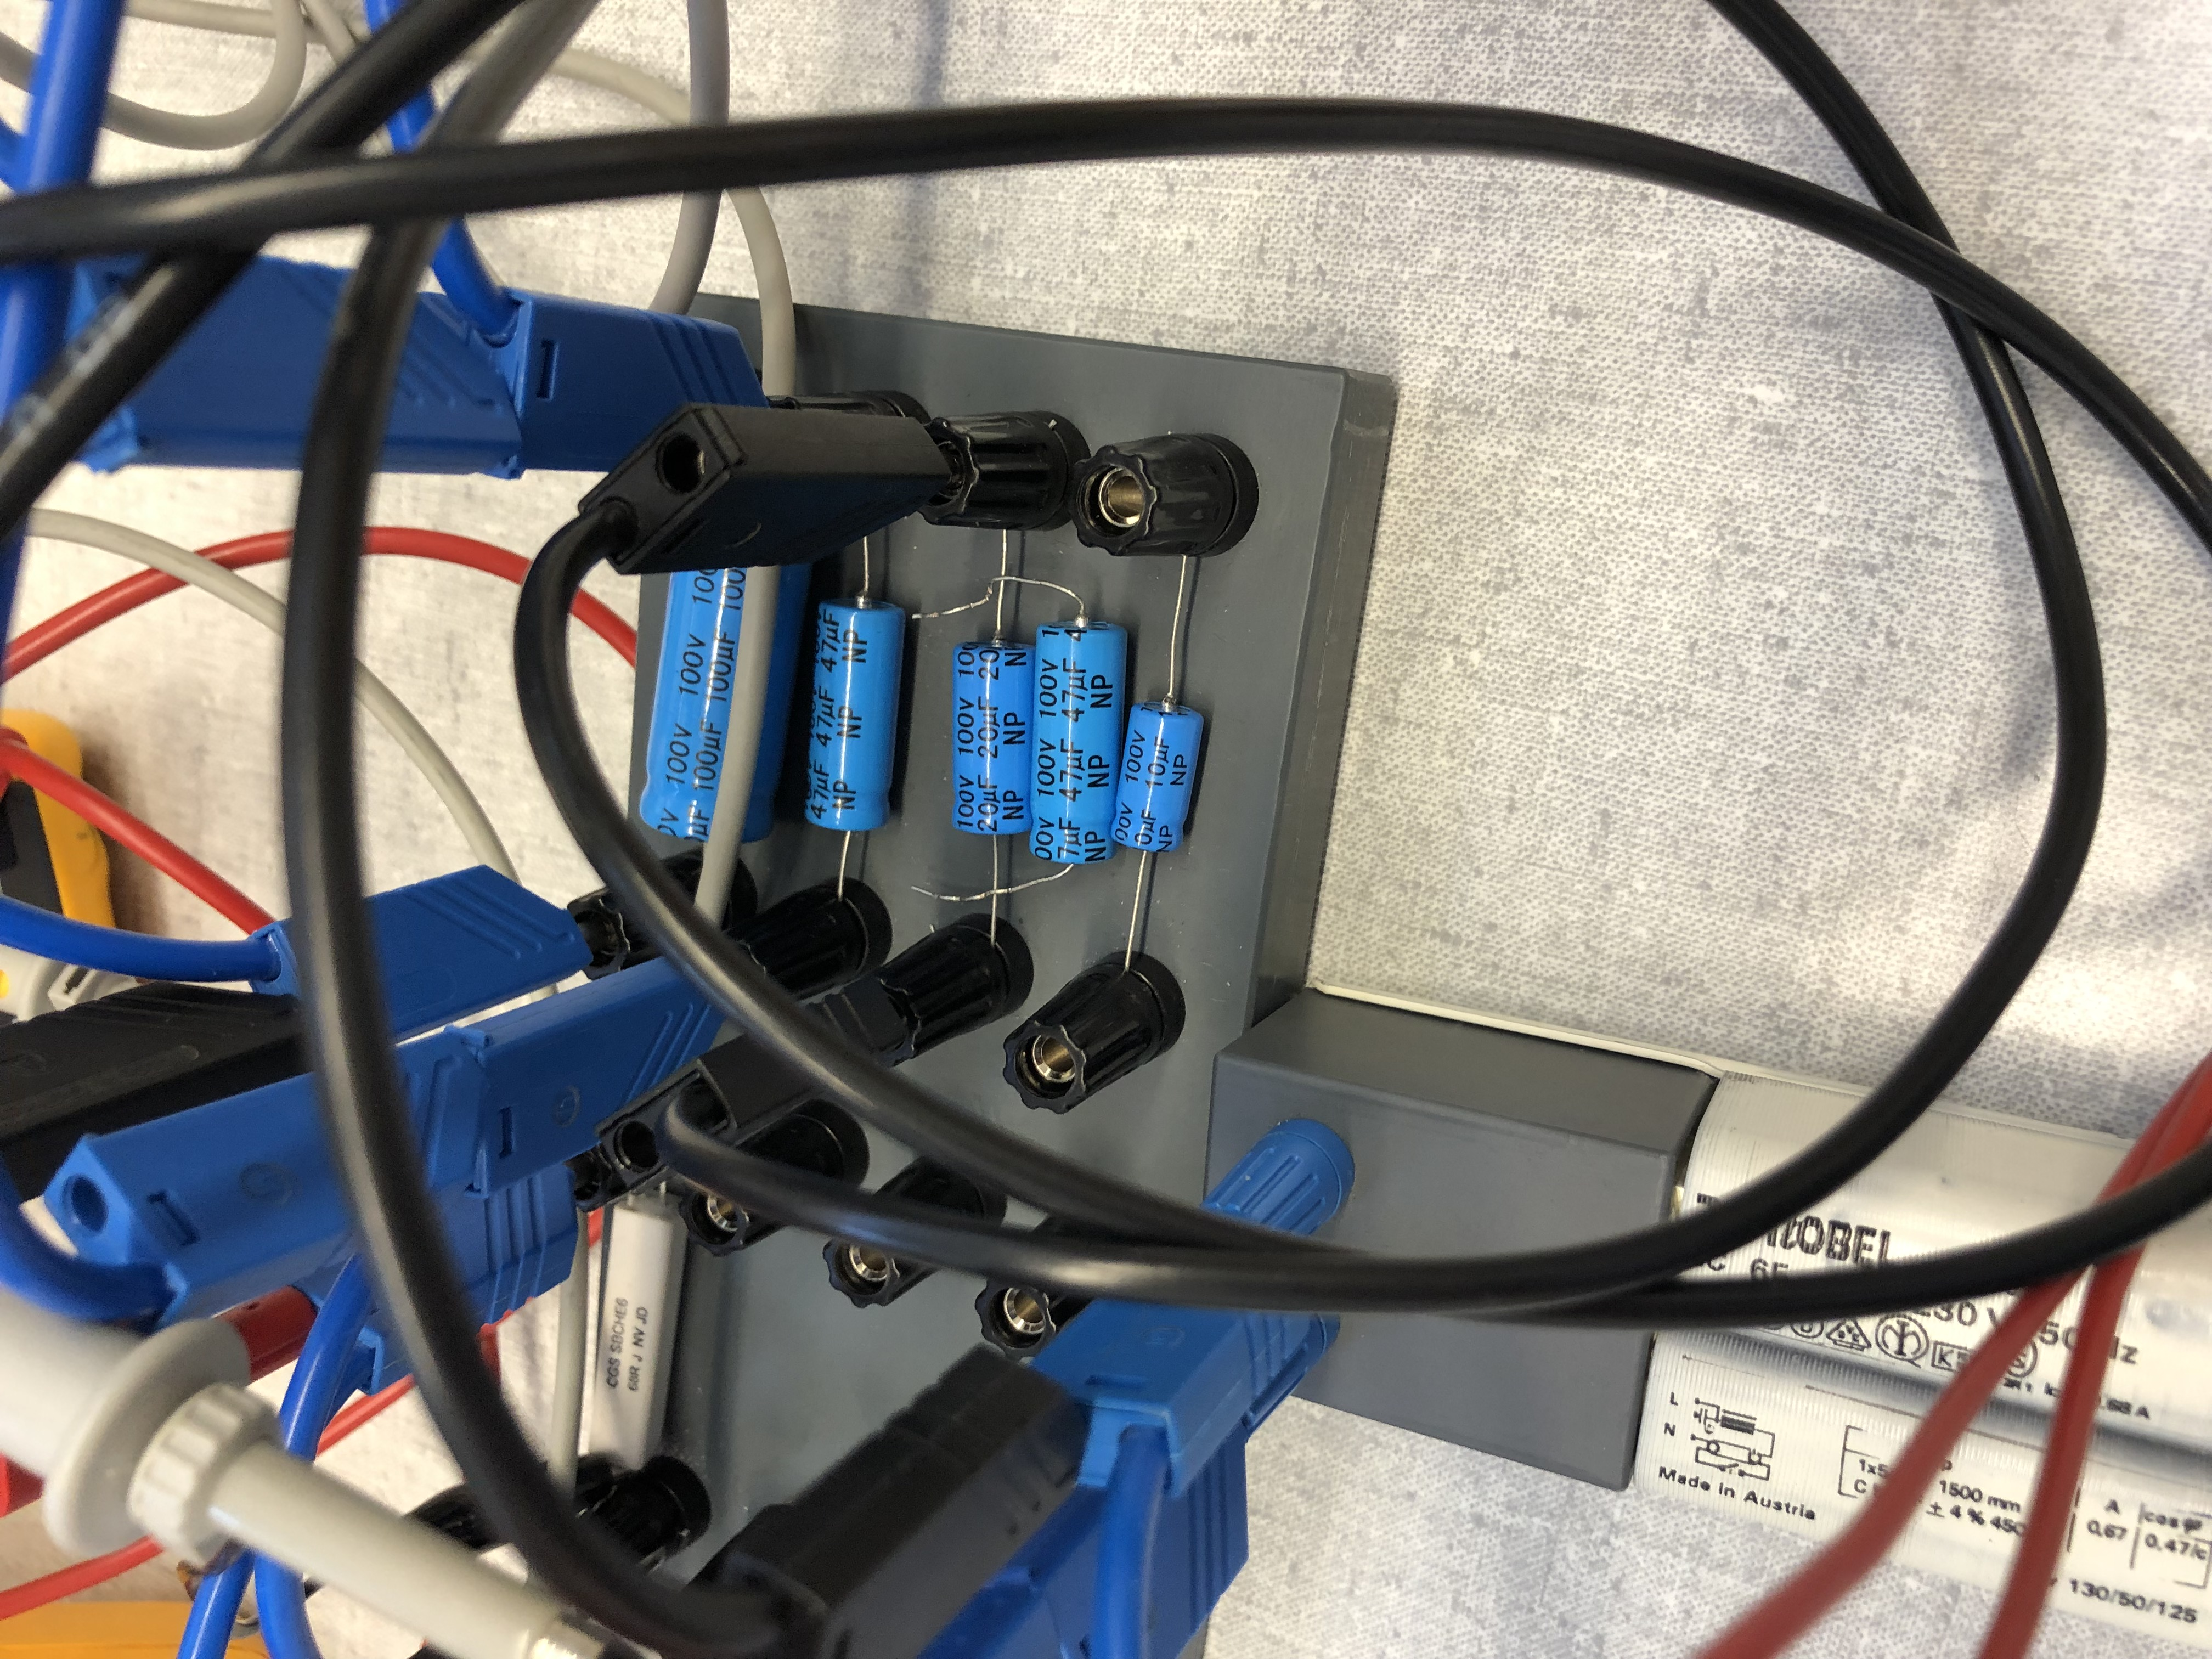
\includegraphics[angle=-90,width=\textwidth]{kap_losung}
		\captionof{figure}{Finale Schaltung der Kapazitäten}
		\label{fig:kap_losung}
	\end{minipage}
\end{center}

\newpage

Das so erhaltene Signal, welches am Oszilloskop angezeigt wird, ist in \autoref{fig:oszi_6_214} sichtbar.

\begin{center}
	\begin{minipage}[t]{0.7\textwidth}
		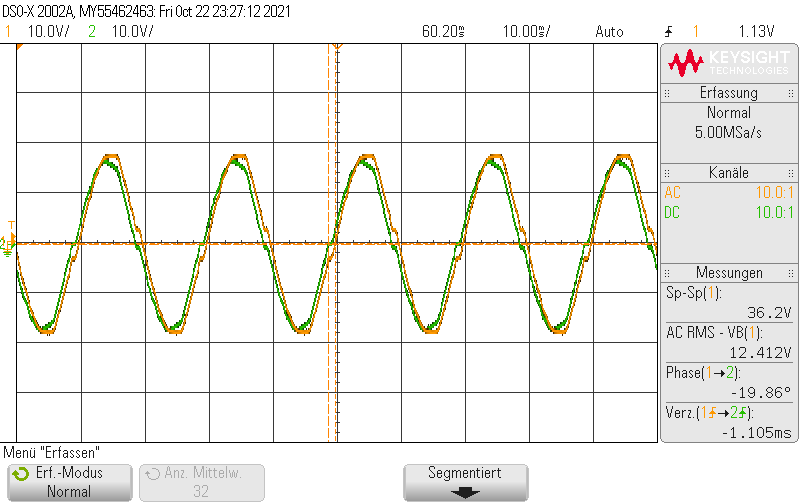
\includegraphics[width=\textwidth]{Phasenzeug/scope_21}
		\captionof{figure}{Vom Oszilloskop aufgezeichnetes Signal bei einem Kondensator mit einer gesamten Kapazität von 214 $\mu$ Farad}
		\label{fig:oszi_6_214}
	\end{minipage}
\end{center}

Die abgelesenen Daten der Messgeräte sind in folgender \autoref{tab:6_214} sichtbar.

\begin{table}[H]
	\captionof{table}{Abgelesene Werte bei Verwendung des Kondensators mit einer
		gesamten Kapazität von 214 $\mu$ Farad \\ $U_{L}$ \dots abgelesener Wert der
		Spannung an der Spule in V, Unsicherheit \cite{fluke} \\ $U_{R}$ \dots abgelesener
		Wert der Spannung am Widerstand in V, Unsicherheit \cite{fluke} \\ $U_{T}$ \dots
		abgelesener Wert der Spannung am Trafo in V, Unsicherheit \cite{fluke} \\ $I_{ges}$
		\dots abgelesener Wert des gesamten Stroms in mA, Unsicherheit \cite{ttimeter} \\
		$I_{C}$ \dots abgelesener Wert des Stroms durch den Kondensator in mA,
		Unsicherheit \cite{ttimeter}}
	\begin{center}
		\begin{tabular}{|c|c|c|c|c|} \hline
			{}          & \textbf{Typ} & \textbf{Wert}      \\ \hline
			Voltmeter   & $U_{L}$      & \SI{2.69(3)}{\V}   \\
			            & $U_{R}$      & \SI{11.78(15)}{\V} \\
			            & $U_{T}$      & \SI{12.76(16)}{\V} \\ \hline
			Amperemeter & $I_{ges}$    & \SI{180(5)}{\mA}   \\
			            & $I_{C}$      & \SI{190(5)}{\mA}   \\ \hline
		\end{tabular}
		\label{tab:6_214}
	\end{center}
\end{table}




\newpage


\section{Auswertung}

\noindent Um zu sehen wie sich die Unsicherheit der Messungen bis in die Ergebnisse
fortplanzt, ist \autoref{eq:Unsicherheitsfortpflanzung} verwendet worden.
Die Grundlagen dieser Gleichung stammen von den Powerpointfolien von
GUM.\cite{WolfgangKessel2004} Die Verallgemeinerung ist von Wikipedia entnommen
worden \cite{2020Fehler}.
Für die Auswertung ist die Progammiersprache Python im speziellen das
Packet \verb#scipy#, zur Hilfe genommen worden.

\begin{equation}
	\label{eq:Unsicherheitsfortpflanzung}
	V_y = J(x) \cdot V_x \cdot J^{T}(x)
\end{equation}

\noindent Wobei $V_y$ und $V_x$ die Kovarianzmatrizen von den Vektoren $\bm{y}$ und $\bm{x}$ sind.
$\bm{x}$ ist der Vektor der Eingangsvariablen und $\bm{y}$ ist der Vektor der Ausgangsvariablen.
$J$ ist die Jakobimatrix der vektorwertigen Funktion $\bm{y} = \vec{F}(\bm{x})$.
So lassen sich die Komponenten der Matrix relativ einfach anschreiben $J_{ij}(x) = \frac{\partial{y_i}}{\partial{x_j}}(x)$.
Damit man die Unsicherheit der einzelnen Variablen $y_i$ bekommt, muss nur die Quadratwurzel des i-ten Diagonalelementes der
$\bm{y}$-Kovarianzmatrix genommen werden $u_i= \sqrt{\mathrm{diag}(V_y)_i}$.
Da in diesem Experiment meistens nur skalare Funktionen untersucht werden, vereinfacht
sich die \autoref{eq:Unsicherheitsfortpflanzung} dramatisch und die Unsicherheit
der Variable $y$ lässt sich einfach so berechnen:

\begin{equation}
	\label{eq:graduncentainty}
	u_y = \sqrt{\mathrm{grad} y^T \cdot V_x \cdot \mathrm{grad} y}
\end{equation}

\vspace{2mm}

Unter Verwendung der ``discrete fourier series`` mit nur dem ersten Term ist
die Phase der Schwingung zusätzlich berechnet worden \cite{welligkeitfourier}.

Diese wurde gemacht damit es als Vergleich mit dem vom Oszilloskop errechneten
Wert dienen kann. Diese Phasenversätze sind den Bildern beigefügt worden.


\subsection{Anzeige von unterschiedlichen Spannungsmessinstrumenten}

Betrachtet man die verschiedenen Messwerte aus \autoref{tab:1b} so stellt man
fest, dass verschiedene Messgeräte unterschiedliche Werte für die selbe
Spannung liefern.



\subsection{Phasenlage von Strom und Spannung an einem Kondensator}

Zunächst muss die Phasenverschiebung zwischen Kondensatorspannung und –strom gefunden werden.
Dazu wird der Strom $I$ durch den Spannungsabfall am Widerstand nach folgender Formel berechnet.

\begin{equation}
	I = \frac{U_{CH1}}{R1}
	\label{eq:i}
\end{equation}

Der so erhaltene Strom, sowie die Spannung, die invertiert wurde, wurden nun geplottet, was in folgender \autoref{fig:kondensatorstromvor} sichtbar ist.

\begin{center}
	\begin{minipage}[t]{0.8\textwidth}
		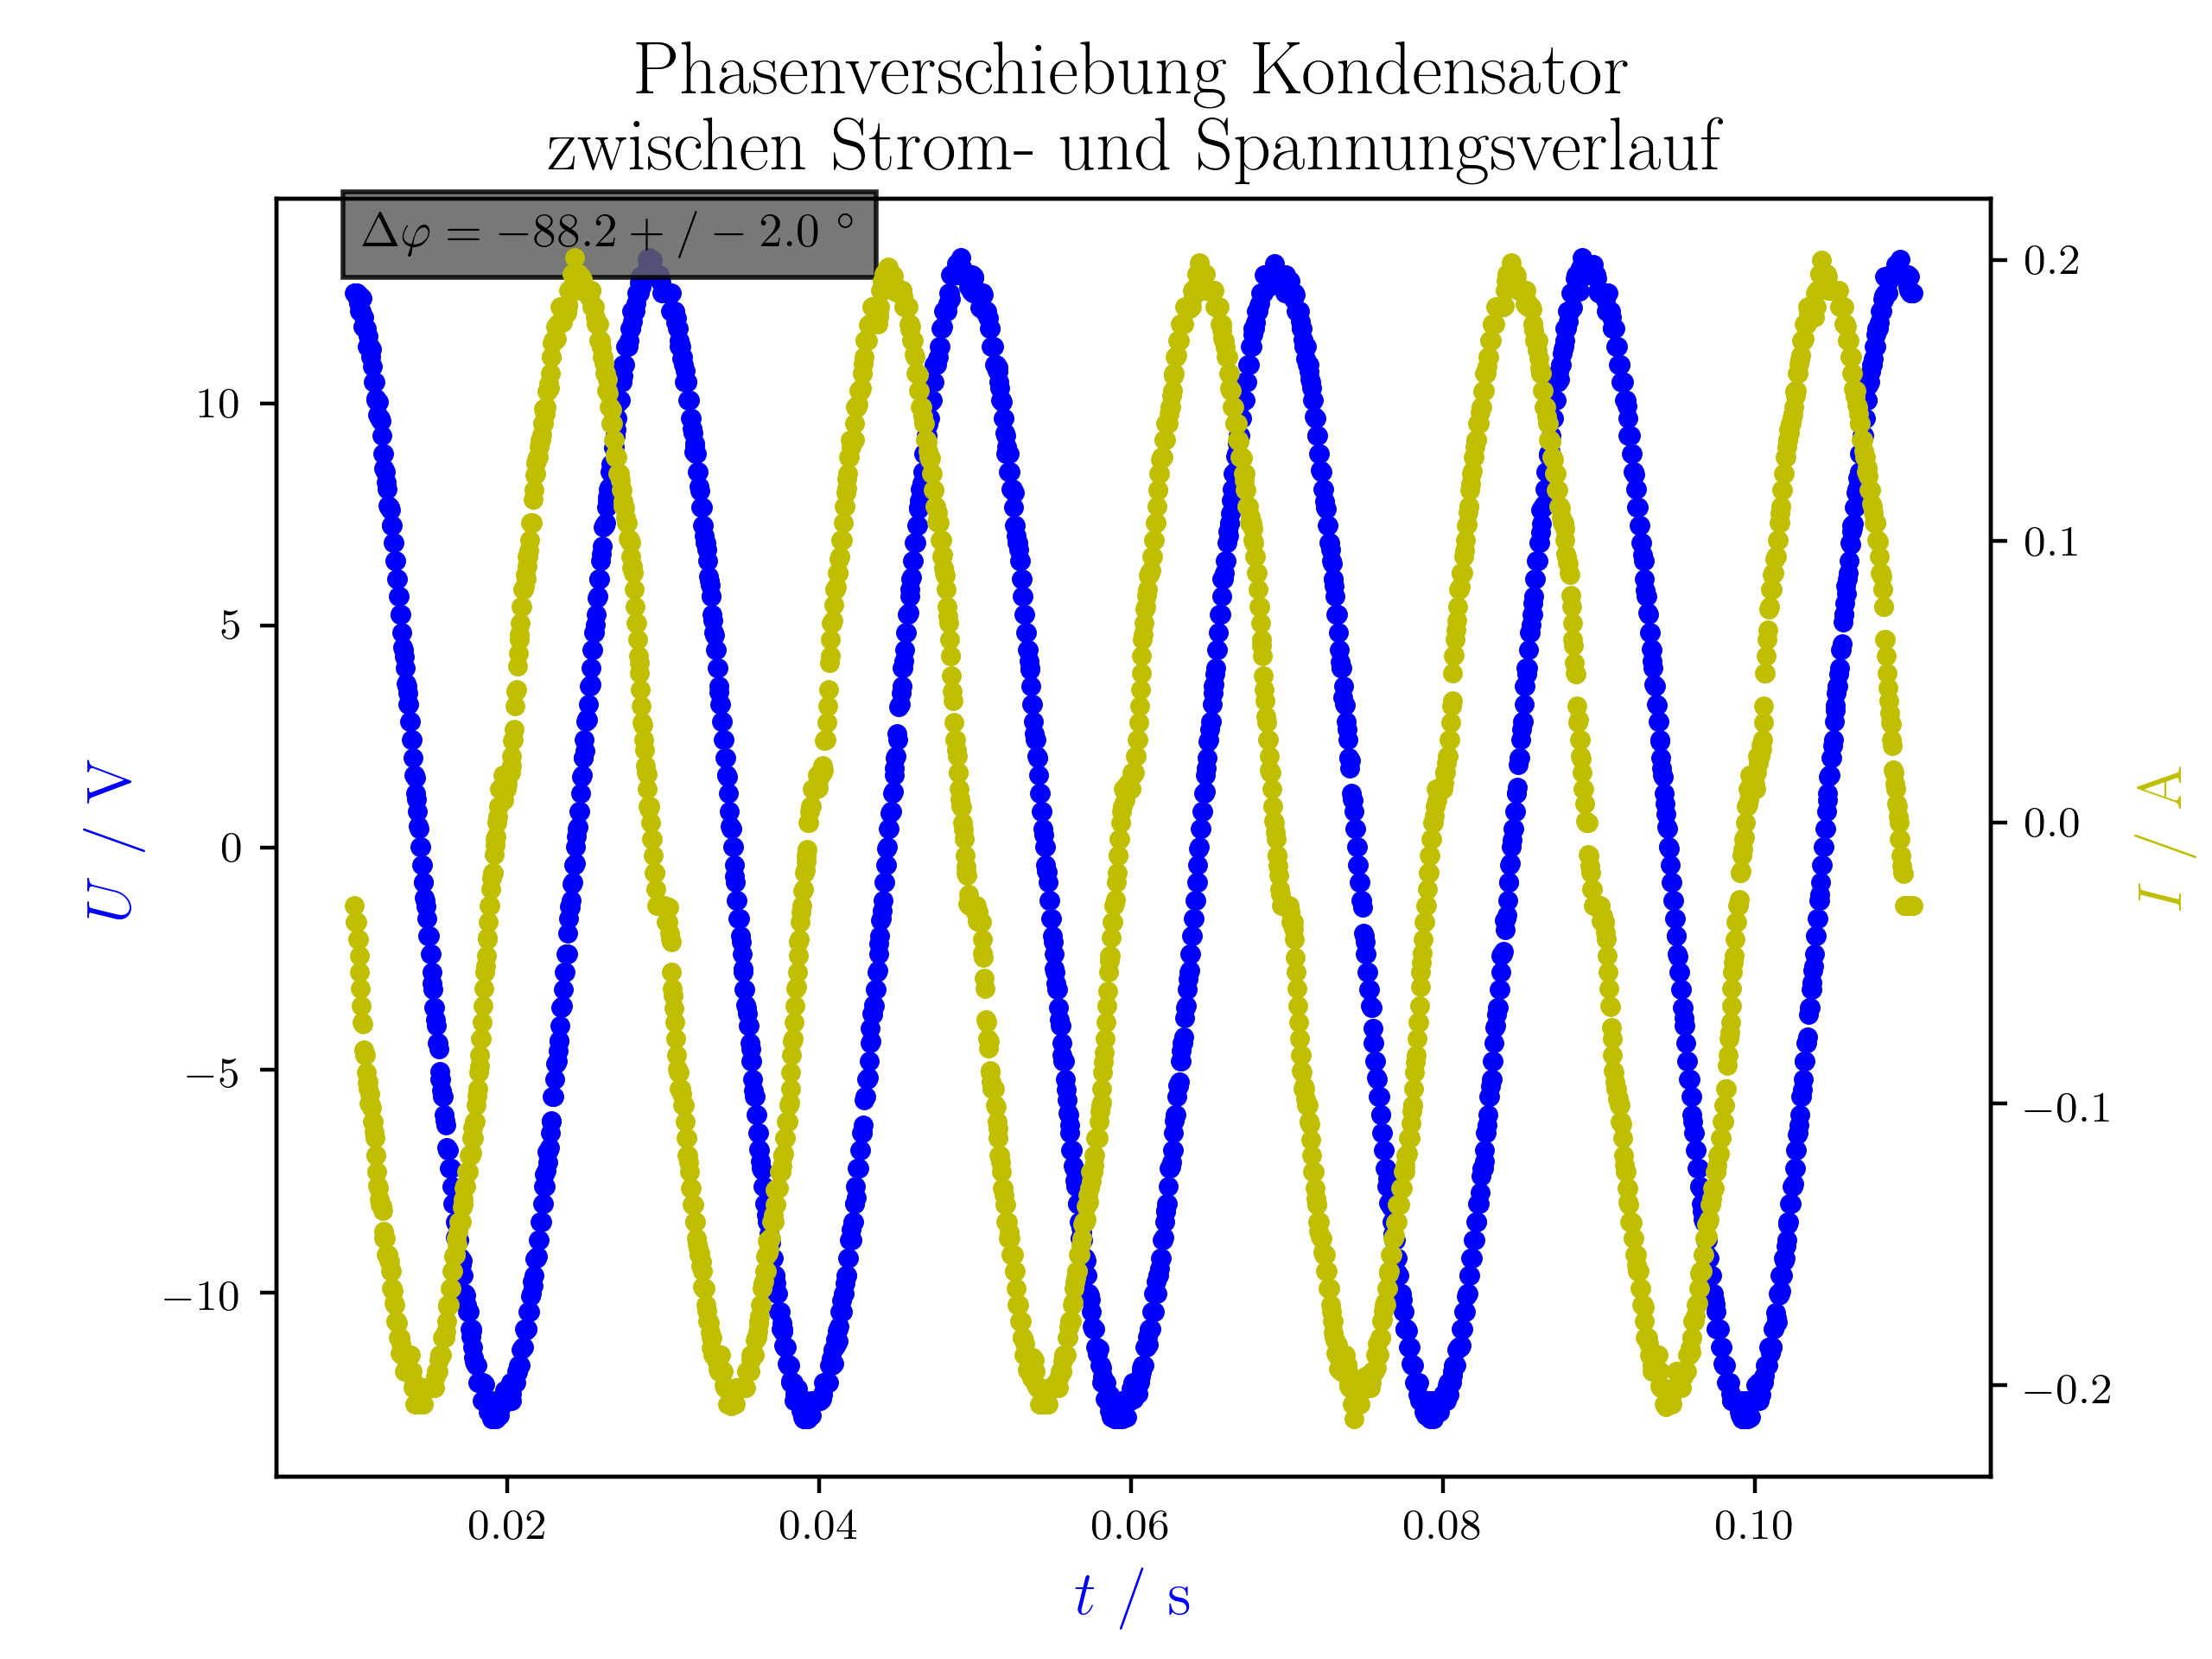
\includegraphics[width=\textwidth]{./figures/phaseleistung/Versuch2/phaseshiftcap.png}
		\captionof{figure}{Strom und Spannungsverlauf des Kondensators, anhand denen die Phasenverschiebung sichtbar wird}
		\label{fig:kondensatorstromvor}
	\end{minipage}
\end{center}

Der genaue Winkel der Phasenverschiebung wurde anhand des Oszilloskops, mit der
jeweiligen Einstellung, bestimmt und beträgt einen Wert von -86.25°, wie in
\autoref{fig:phase_2} sichtbar.

\begin{center}
	\begin{minipage}[t]{0.7\textwidth}
		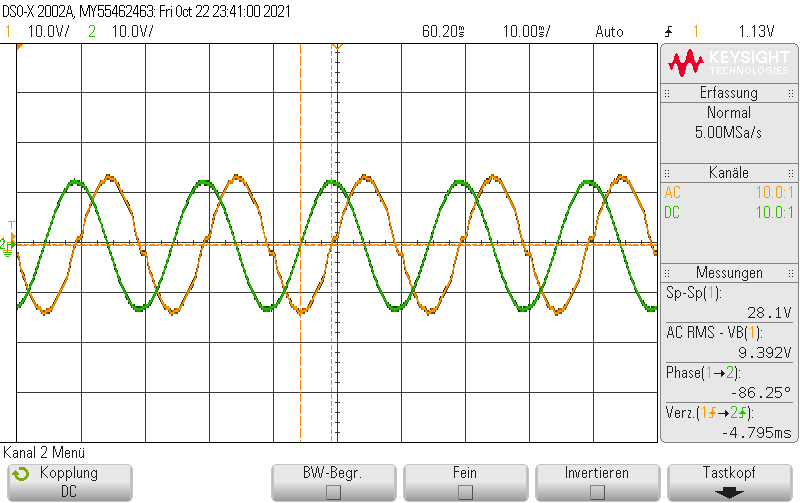
\includegraphics[width=\textwidth]{Phasenzeug/scope_22}
		\captionof{figure}{Vom Oszilloskop aufgezeichnetes Signal bei dem der Phasenwinkel angezeigt wird}
		\label{fig:phase_2}
	\end{minipage}
\end{center}

\newpage

\subsection{Phasenlage von Strom und Spannung an einer Spule}


Um die Phasenverschiebung zwischen Spulenspannung und –strom zu bestimmen, wird der Strom zunächst durch den Spannungsabfall am Widerstand nach \autoref{eq:i} berechnet.

\vspace{2mm}

Nun wird dieser Wert für den Strom zusammen mit den der Spannung, diesmal jedoch nicht invertiert, geplottet, was folgende \autoref{fig:phaseshiftind} ergibt.

\begin{center}
	\begin{minipage}[t]{0.8\textwidth}
		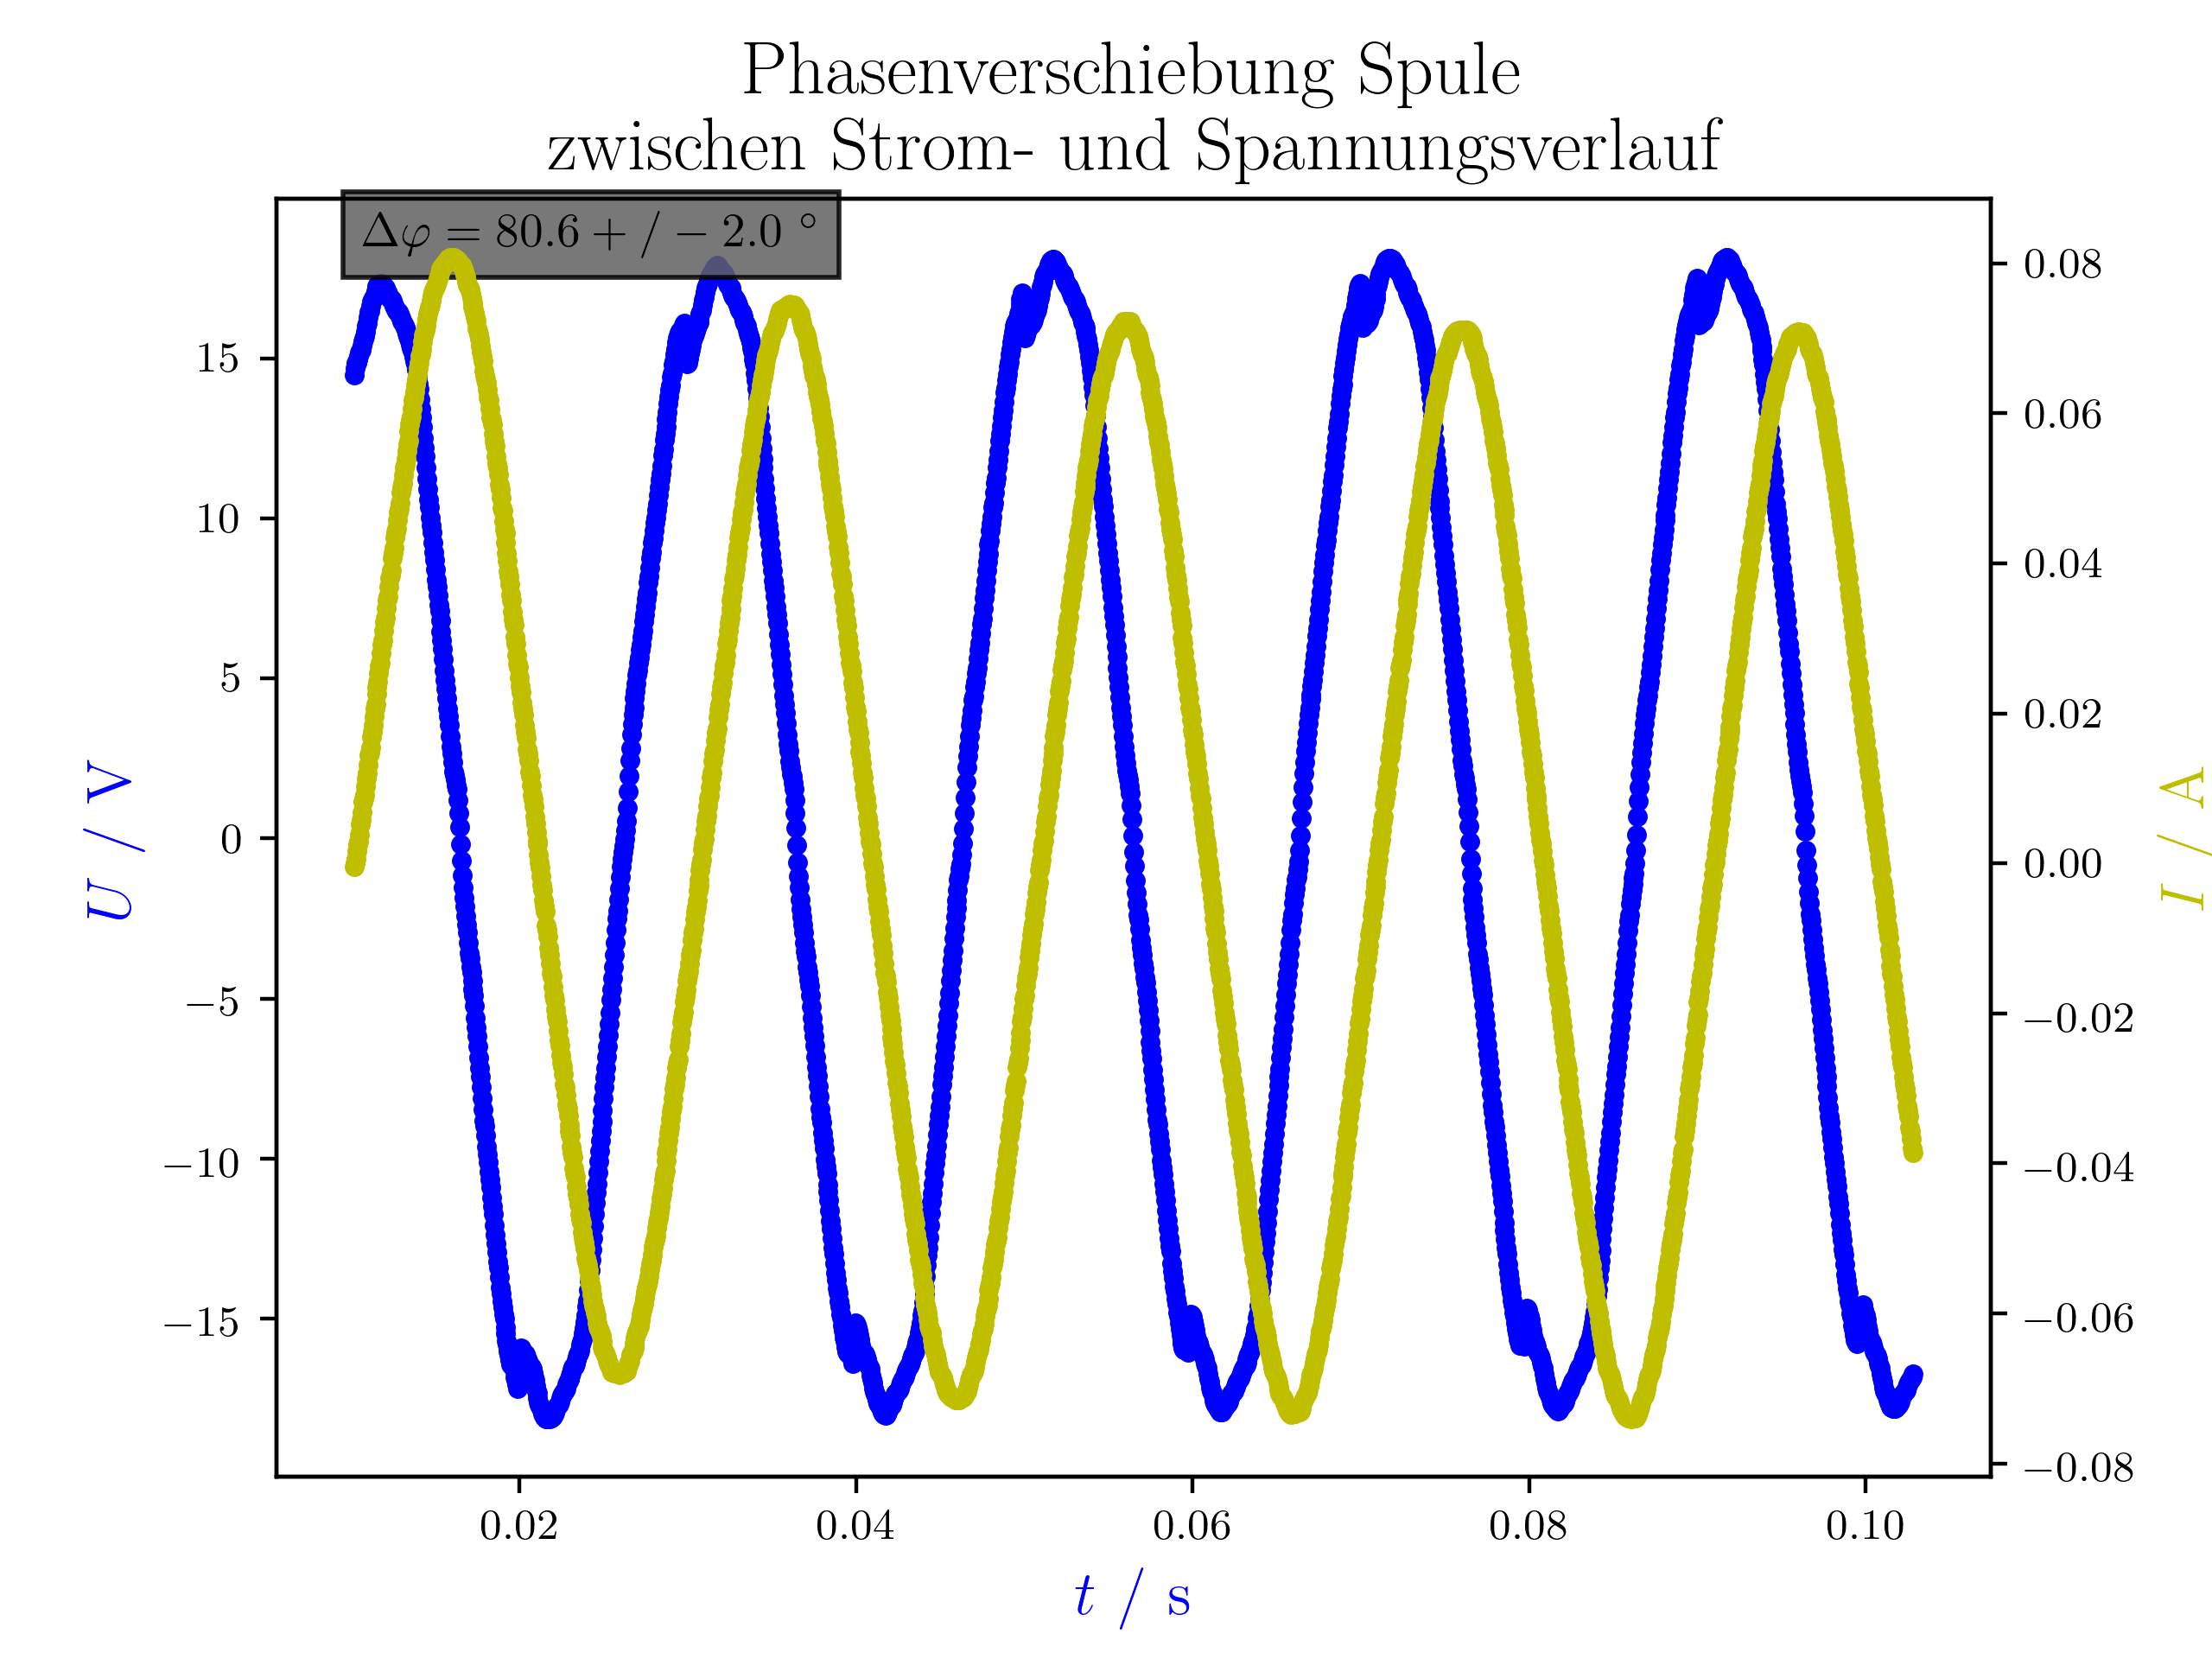
\includegraphics[width=\textwidth]{./figures/phaseleistung/Versuch3/phaseshiftind.png}
		\captionof{figure}{Strom und Spannungsverlauf der Spule, anhand denen die Phasenverschiebung sichtbar wird}
		\label{fig:phaseshiftind}
	\end{minipage}
\end{center}

Der erhaltene Wert der Phasenverschiebung laut Oszilloskop beträgt 86.00°,
siehe \autoref{fig:oszi_2_winkel}. Dies deckt sich jedoch nicht mit dem
erhaltenen Wert.
%warum -

\subsection{elektrische Leistung in einer RC-Schaltung}

Zunächst muss wieder die Phasenverschiebung zwischen der Spannung $U_E$ und dem Strom $I$ bestimmt werden.
%sowie das Leistungsdreieck im RC-Kreis.
Die Spannung ist einfach das vom Oszilloskop aufgezeichnete Signal von ``Channel 1``, $U_{CH1}$.
Der Strom wird durch den Spannungsabfall am Widerstand nach \autoref{eq:i} berechnet. Dabei ist zu beachten, dass das richtige Signal des Oszilloskops bei dieser Schaltung an ``Channel 2`` abgegriffen wird, sodass sich für den Strom  $I = \frac{U_{CH2}}{R1}$ ergibt.

\vspace{2mm}

Die erhaltenen Daten wurden in folgender \autoref{fig:phaseshiftrc} geplottet.

\begin{center}
	\begin{minipage}[t]{0.8\textwidth}
		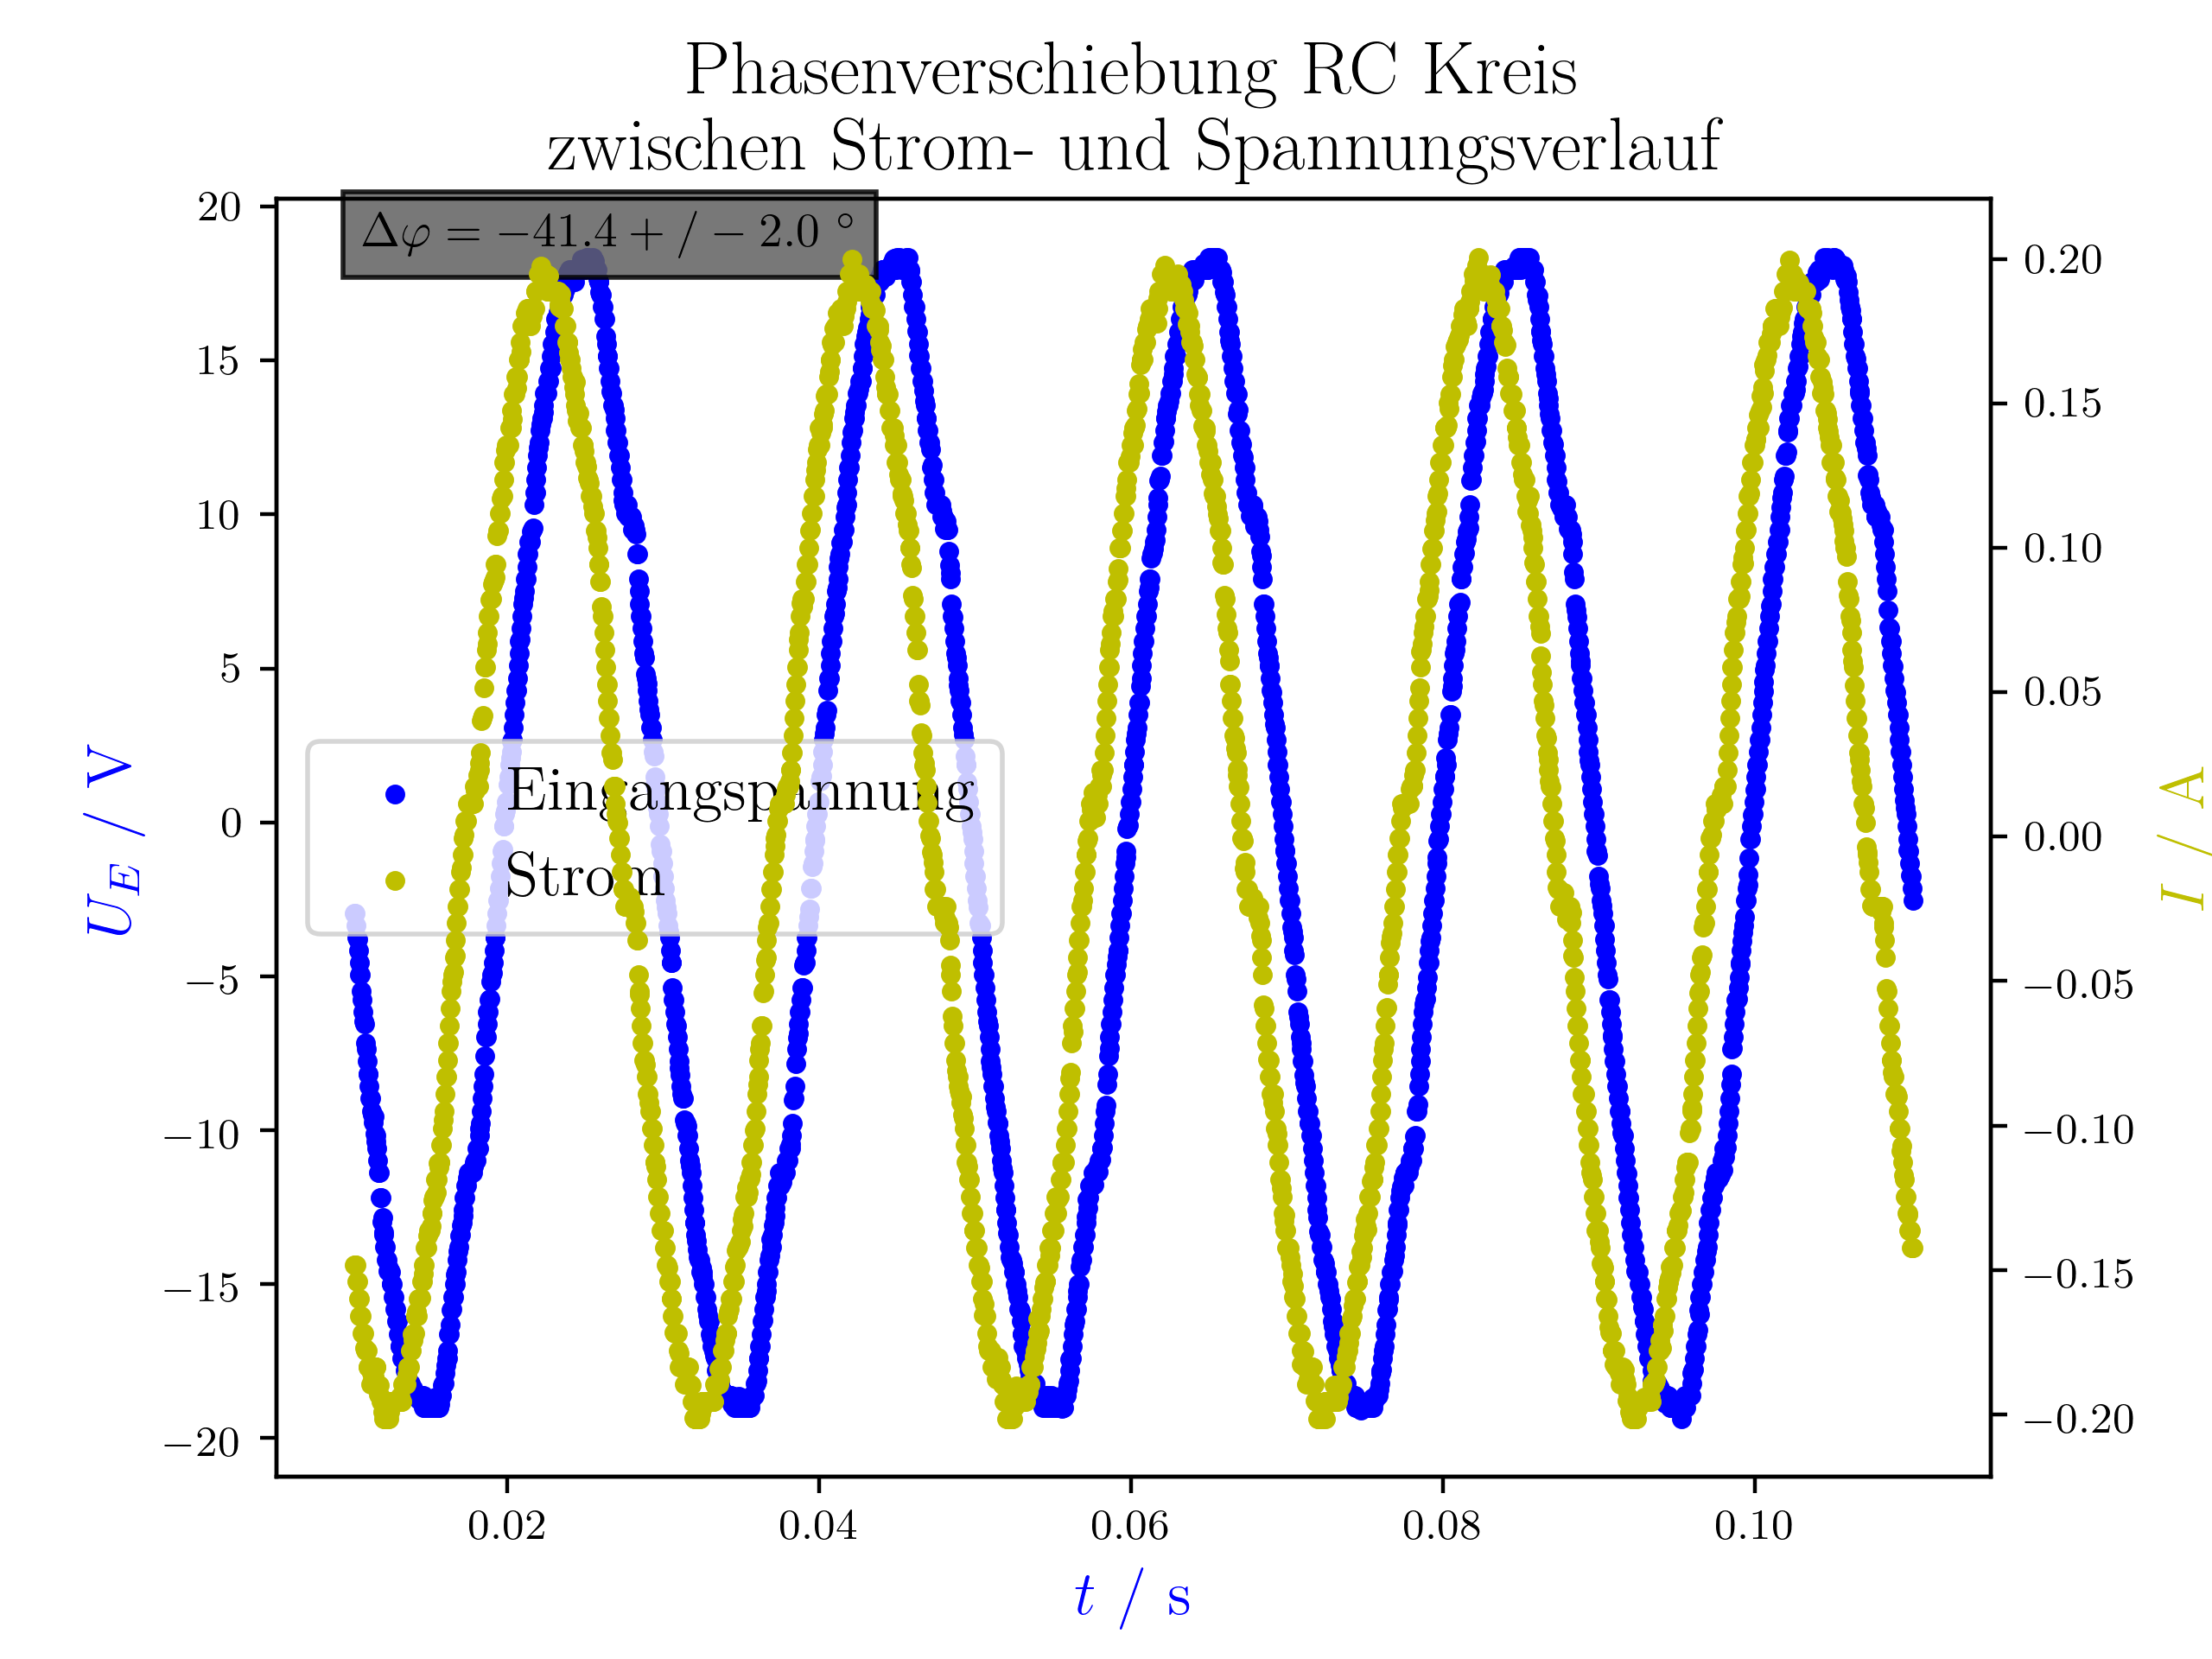
\includegraphics[width=\textwidth]{./figures/phaseleistung/Versuch4/phaseshiftrc.png}
		\captionof{figure}{Phasenverschiebung zwischen Strom und Spannung in RC-Schaltung}
		\label{fig:phaseshiftrc}
	\end{minipage}
\end{center}

Der vom Oszilloskop angezeigte Wert beträgt einen Winkel von - 45.92°, siehe \autoref{fig:oszi_4} und ist wieder nicht im errechneten Intervall enthalten.

Eine andere Möglichkeit den Phasenversatz zu bestimmen ist anhand \autoref{eq:phi}.
Dies liefert mit den Werten aus \autoref{tab:4} einen Phasenwinkel von \SI{-41.8(15)}{\degree}





\subsection{elektrische Leistung in einer RL-Schaltung}

Auch hier muss wieder die Phasenverschiebung zwischen der Spannung $U_E$ und dem Strom $I$ bestimmt werden.
% Leistungsdreieck im RL-Kreis.
Die Spannung und der Strom ergeben sich analog zur RC-Schaltung als $U = U_{CH1}$ und $I = \frac{U_{CH2}}{R1}$.

\vspace{2mm}

Die so erhaltenen Daten wurden in folgender \autoref{fig:phaseshiftrl} geplottet.

\begin{center}
	\begin{minipage}[t]{0.8\textwidth}
		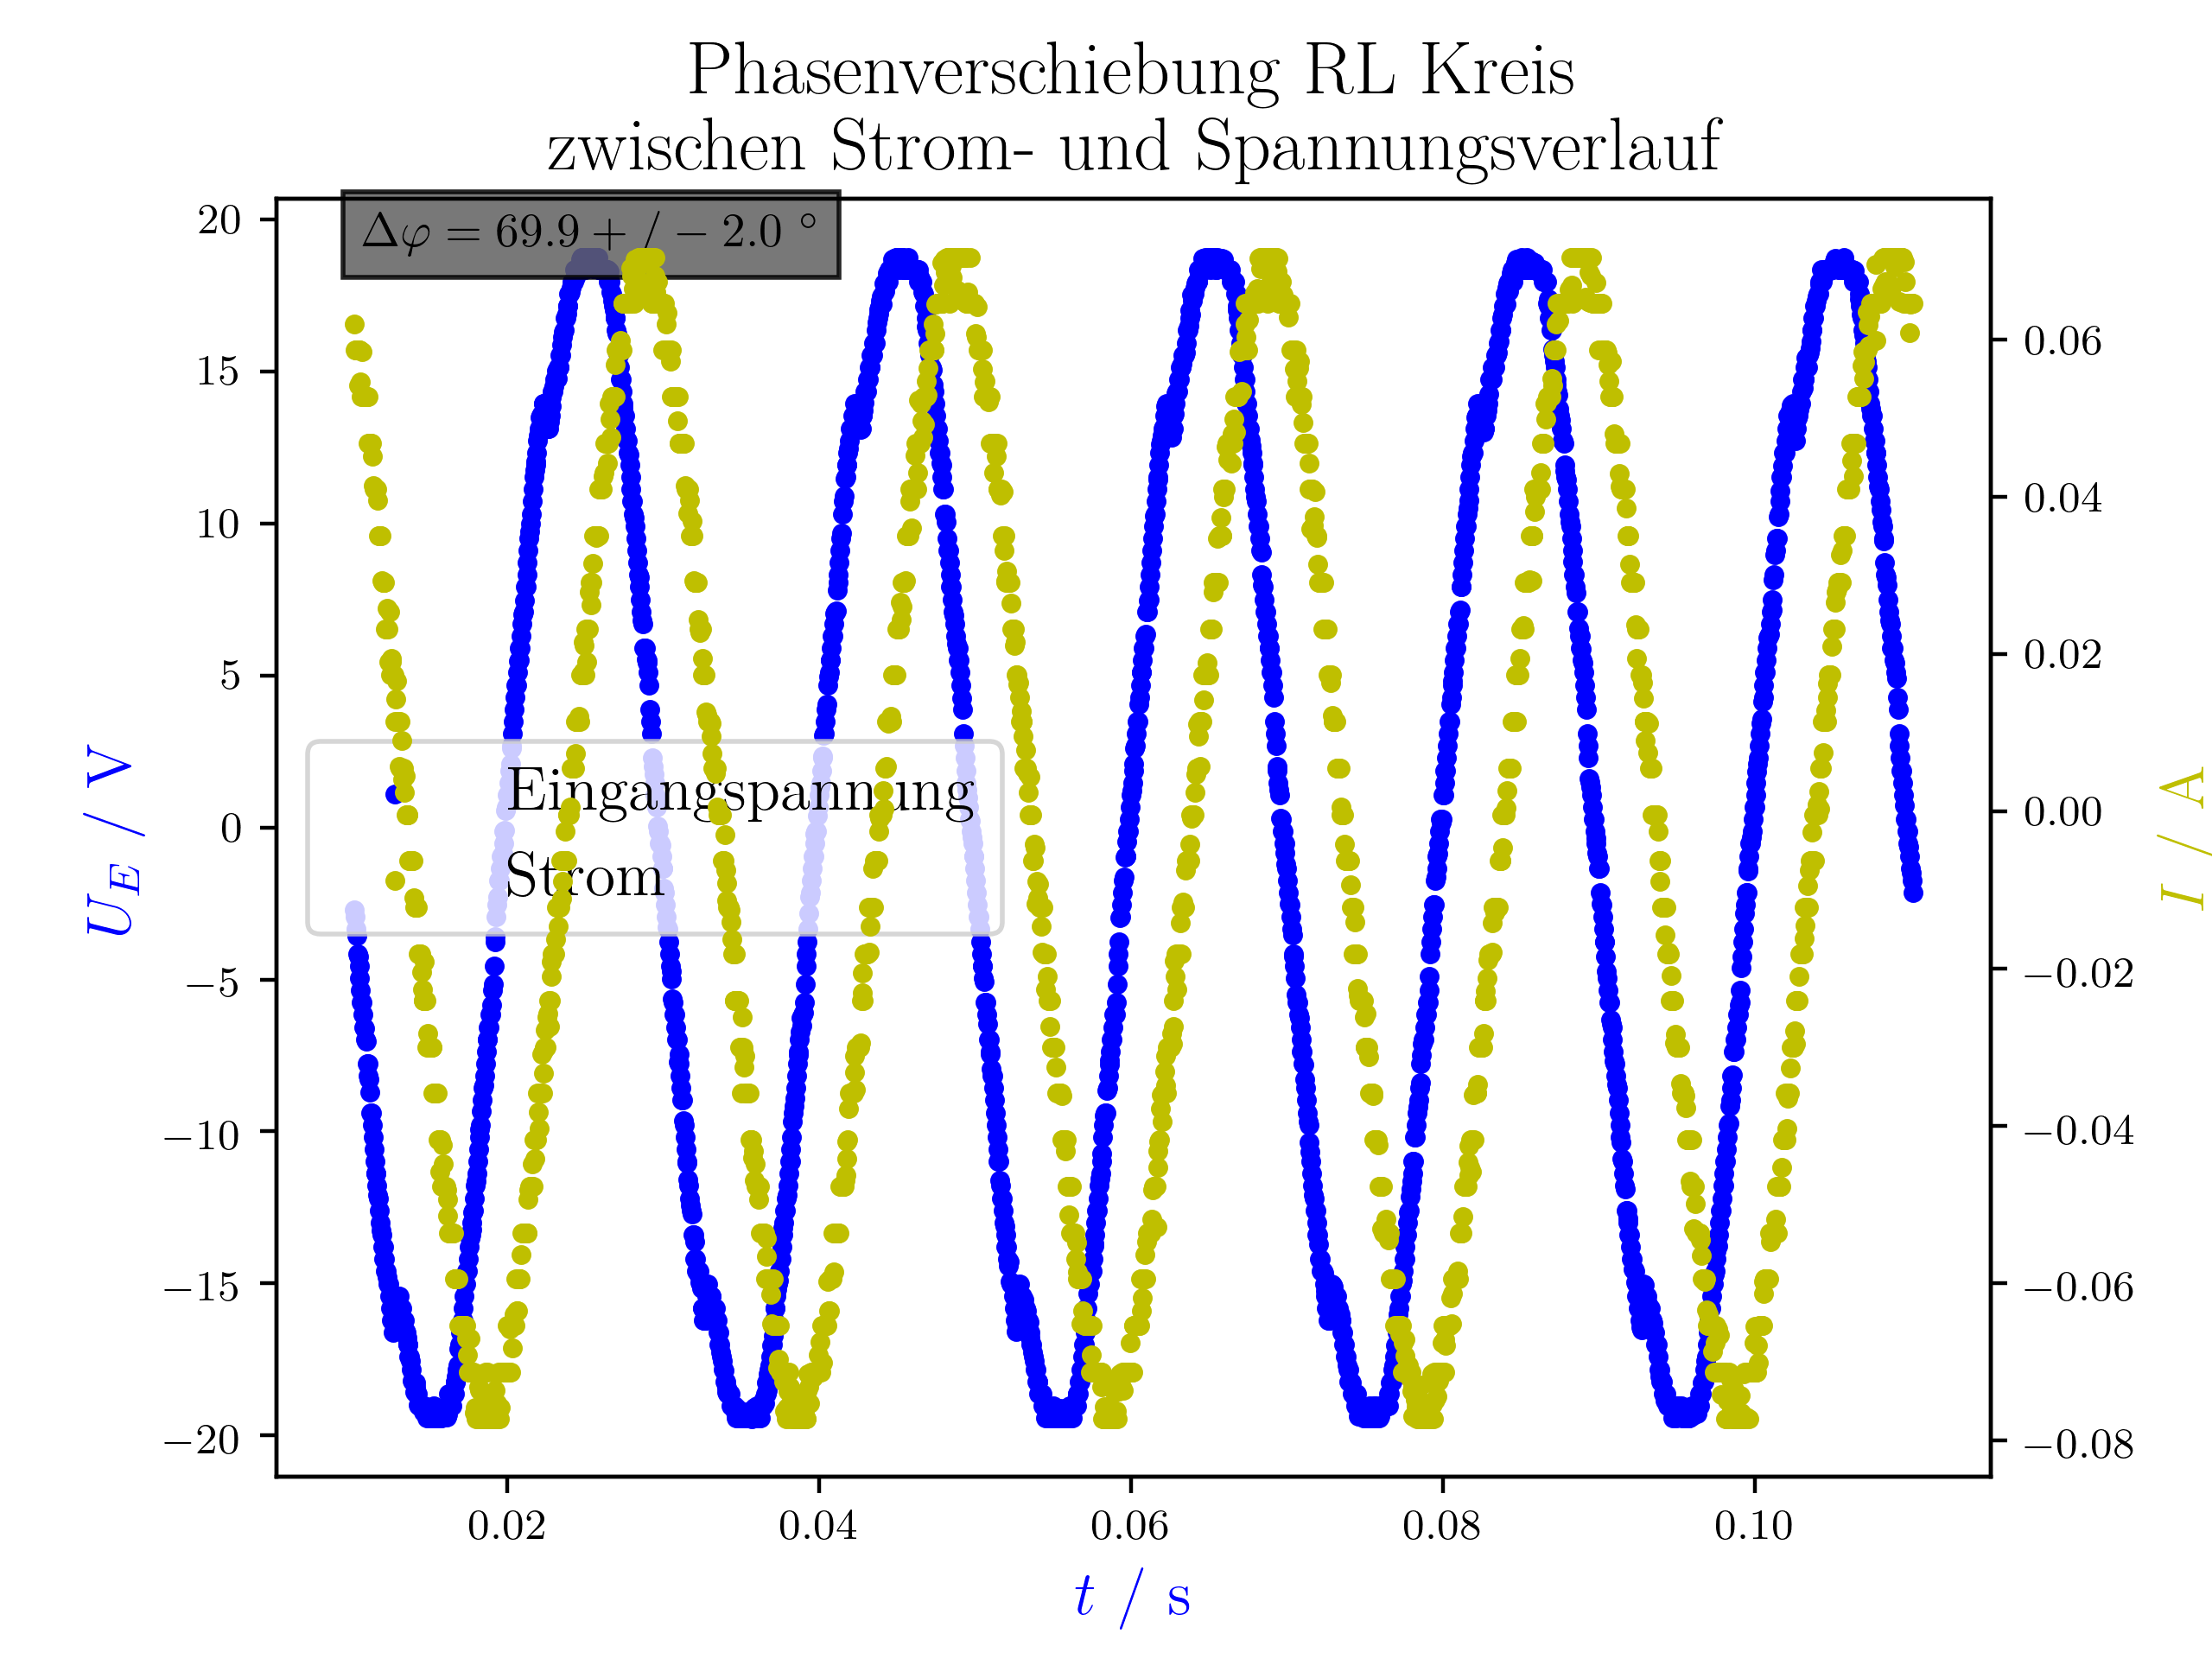
\includegraphics[width=\textwidth]{./figures/phaseleistung/Versuch5/phaseshiftrl.png}
		\captionof{figure}{Phasenverschiebung zwischen Strom und Spannung in RL-Schaltung}
		\label{fig:phaseshiftrl}
	\end{minipage}
\end{center}

Auch hier wurde der Winkel der Phasenverschiebung wieder vom Oszilloskop angezeigt und beträgt einen Winkel von 72.54°, siehe \autoref{fig:oszi_5} und ist wieder nicht im errechneten Intervall enthalten.

Auch hier wurde der Vergleichswert der mithilfe des Powermeter gemessenen Werte aus \autoref{tab:4} und \autoref{eq:phi} bestimmt, was einen Wert von \SI{68(3)}{\degree}.


\subsection{Blindleistungskompensation eines induktiven Verbrauchers}

Unter idealer Blindleistungskompensation versteht man, dass sich der Blindleistungsanteil der Spule und des Kondensators kompensieren. Daher muss $X_L=X_C$ gelten. Unter der Verwendung von \autoref{eq:xc} und \autoref{eq:xl} ergibt sich schließlich:

\begin{align*}
	|X_L|    & = |X_C|                 \\
	\omega L & = \frac{1 }{\omega C}   \\
	C        & = \frac{1 }{\omega^2 L}
\end{align*}

\vspace{2mm}

Da die Induktivität $L$ bekannt ist folgt schließlich:

\begin{align*}
	L                 & = \frac{R \tan{(\Delta \varphi)}}{\omega}  \\
	                  & = \frac{R U_{L_{eff}}}{2\pi f U_{R_{eff}}} \\
	                  & = \SI{828(10)}{\milli\henry}               \\
	\hookrightarrow C & = \SI{12.24(14)}{\micro\farad}
\end{align*}

Die Werte

\begin{align*}
	U_{L_{eff}}= \SI{13.14(17)}{\volt} \\
	U_{R_{eff}} =\SI{3.41(4)}{\volt}
\end{align*}

wurden bei der 5.Aufgabe mit den Fluke-Multimeter gemessen.


\vspace{2mm}

Anhand der vom Oszilloskop aufgezeichneten Daten wurden folgende Graphen für die unterschiedlichen Kapazitäten erzeugt.
Als Wert für die Spannung wurde wieder $U = U_{CH1}$ geplottet. Der Strom erneut durch den Spannungsabfall am Widerstand als $I = \frac{U_{CH2}}{R1}$ berechnet.

\begin{center}
	\begin{minipage}[t]{0.8\textwidth}
		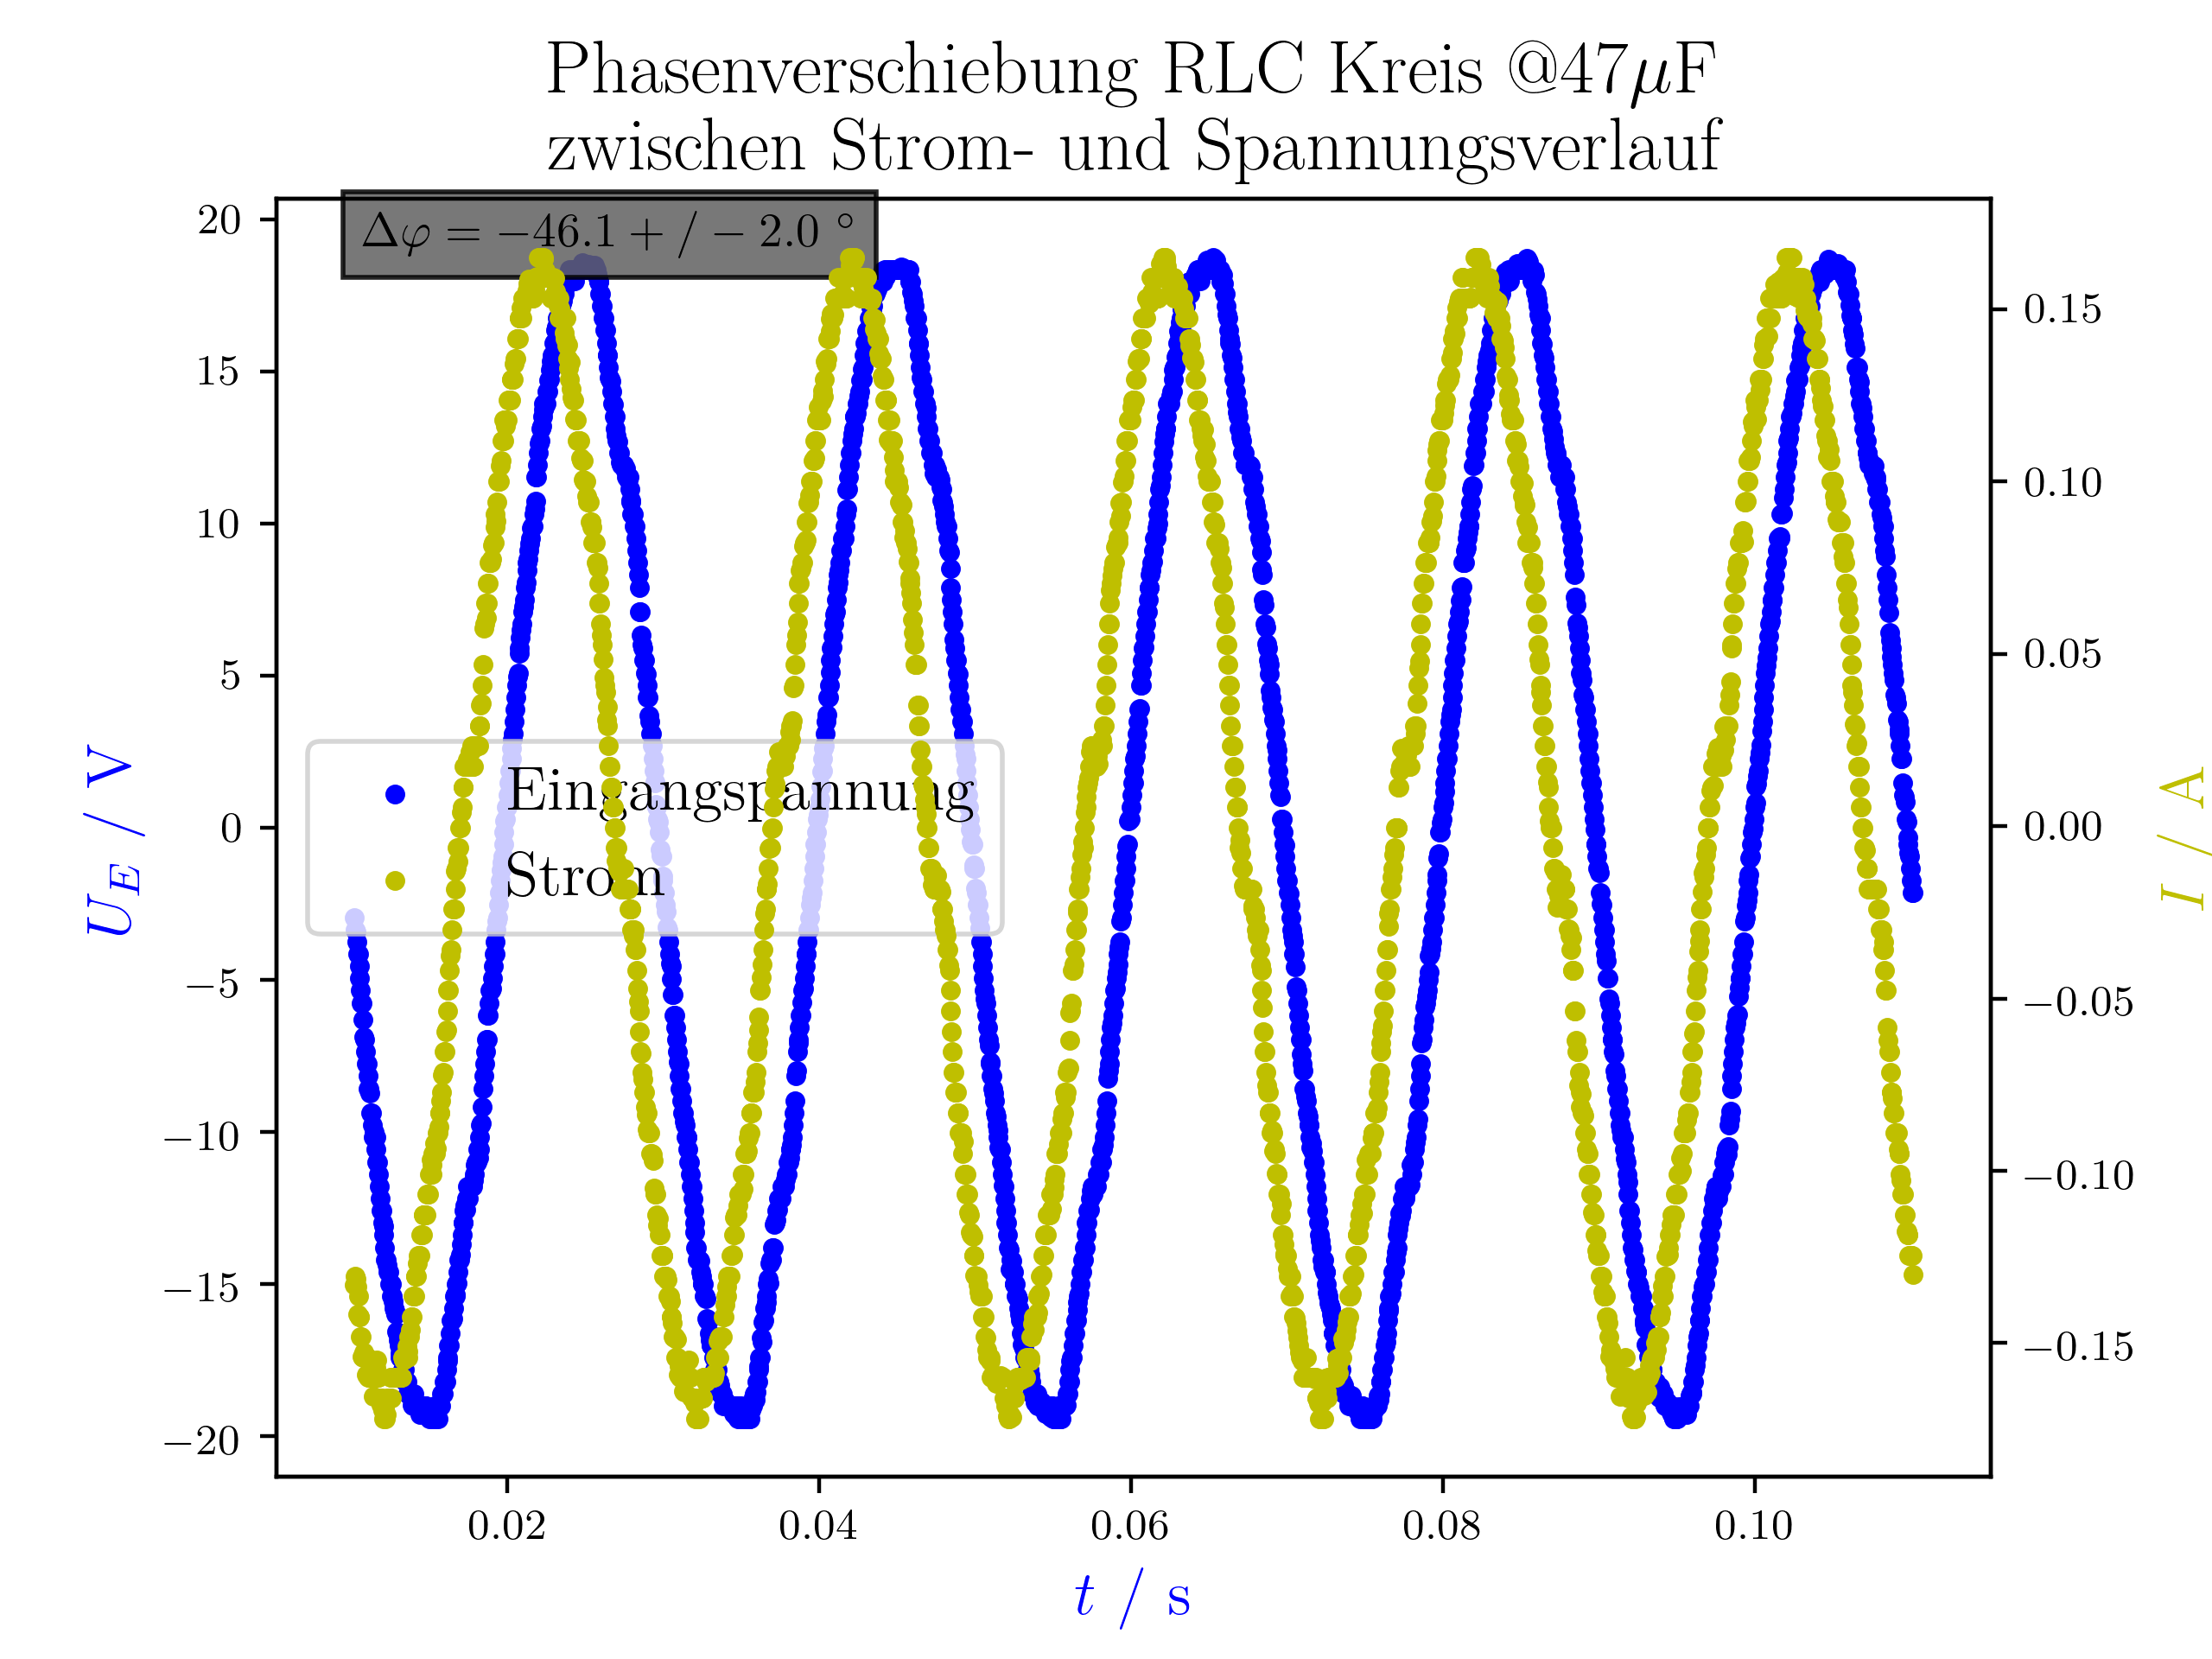
\includegraphics[width=\textwidth]{./figures/phaseleistung/Versuch6/phaseshiftrlc15.png}
		\captionof{figure}{Phasenverschiebung zwischen Strom und Spannung in RLC-Kreis bei einer Kapazität von 47 $\mu$ Farad}
		\label{fig:phaseshiftrlc15}
	\end{minipage}
\end{center}

Der entsprechende Wert der Phasenverschiebung am Oszilloskop beträgt -51.42°, siehe \autoref{fig:oszi_6_47} und ist wieder nicht im erhaltenen Fehlerintervall des errechneten Phasenversatzes enthalten.



\begin{center}
	\begin{minipage}[t]{0.8\textwidth}
		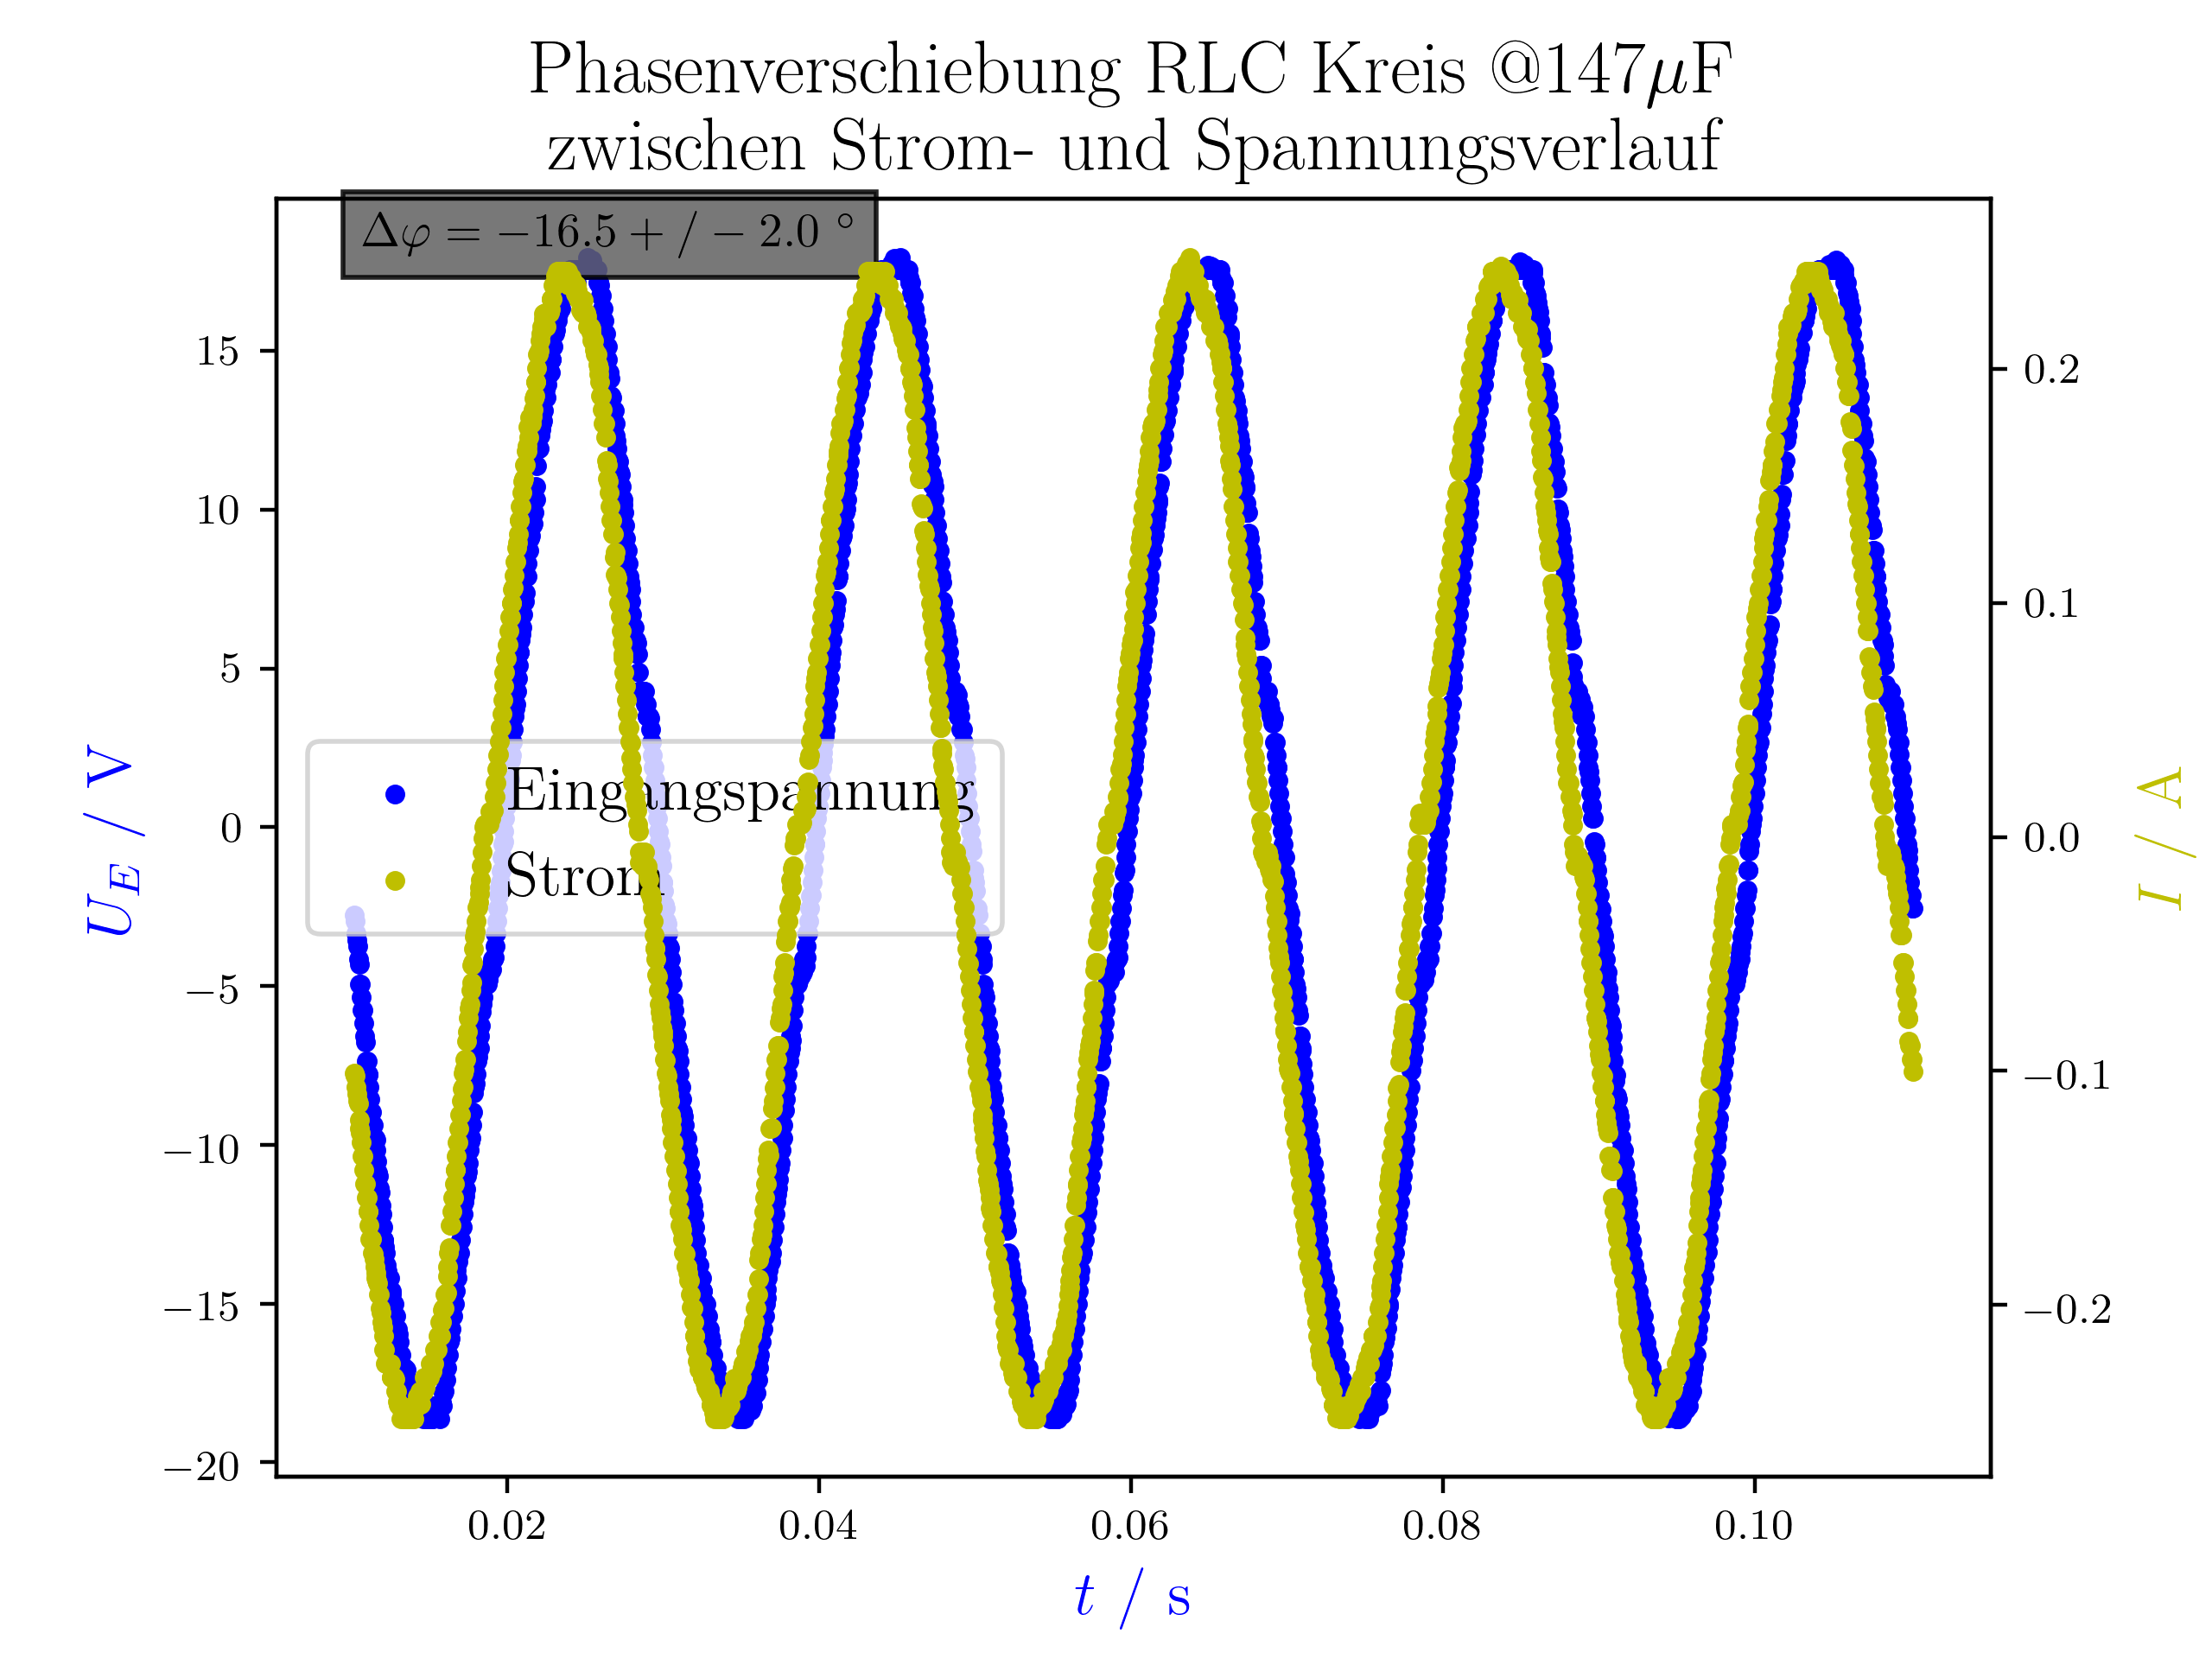
\includegraphics[width=\textwidth]{./figures/phaseleistung/Versuch6/phaseshiftrlc19.png}
		\captionof{figure}{Phasenverschiebung zwischen Strom und Spannung in RLC-Kreis bei einer Kapazität von 147 $\mu$ Farad}
		\label{fig:phaseshiftrlc19}
	\end{minipage}
\end{center}

Der entsprechende Wert der Phasenverschiebung am Oszilloskop beträgt -24.04°, siehe \autoref{fig:oszi_6_147} und ist wieder nicht im erhaltenen Fehlerintervall des errechneten Phasenversatzes enthalten.


\begin{center}
	\begin{minipage}[t]{0.8\textwidth}
		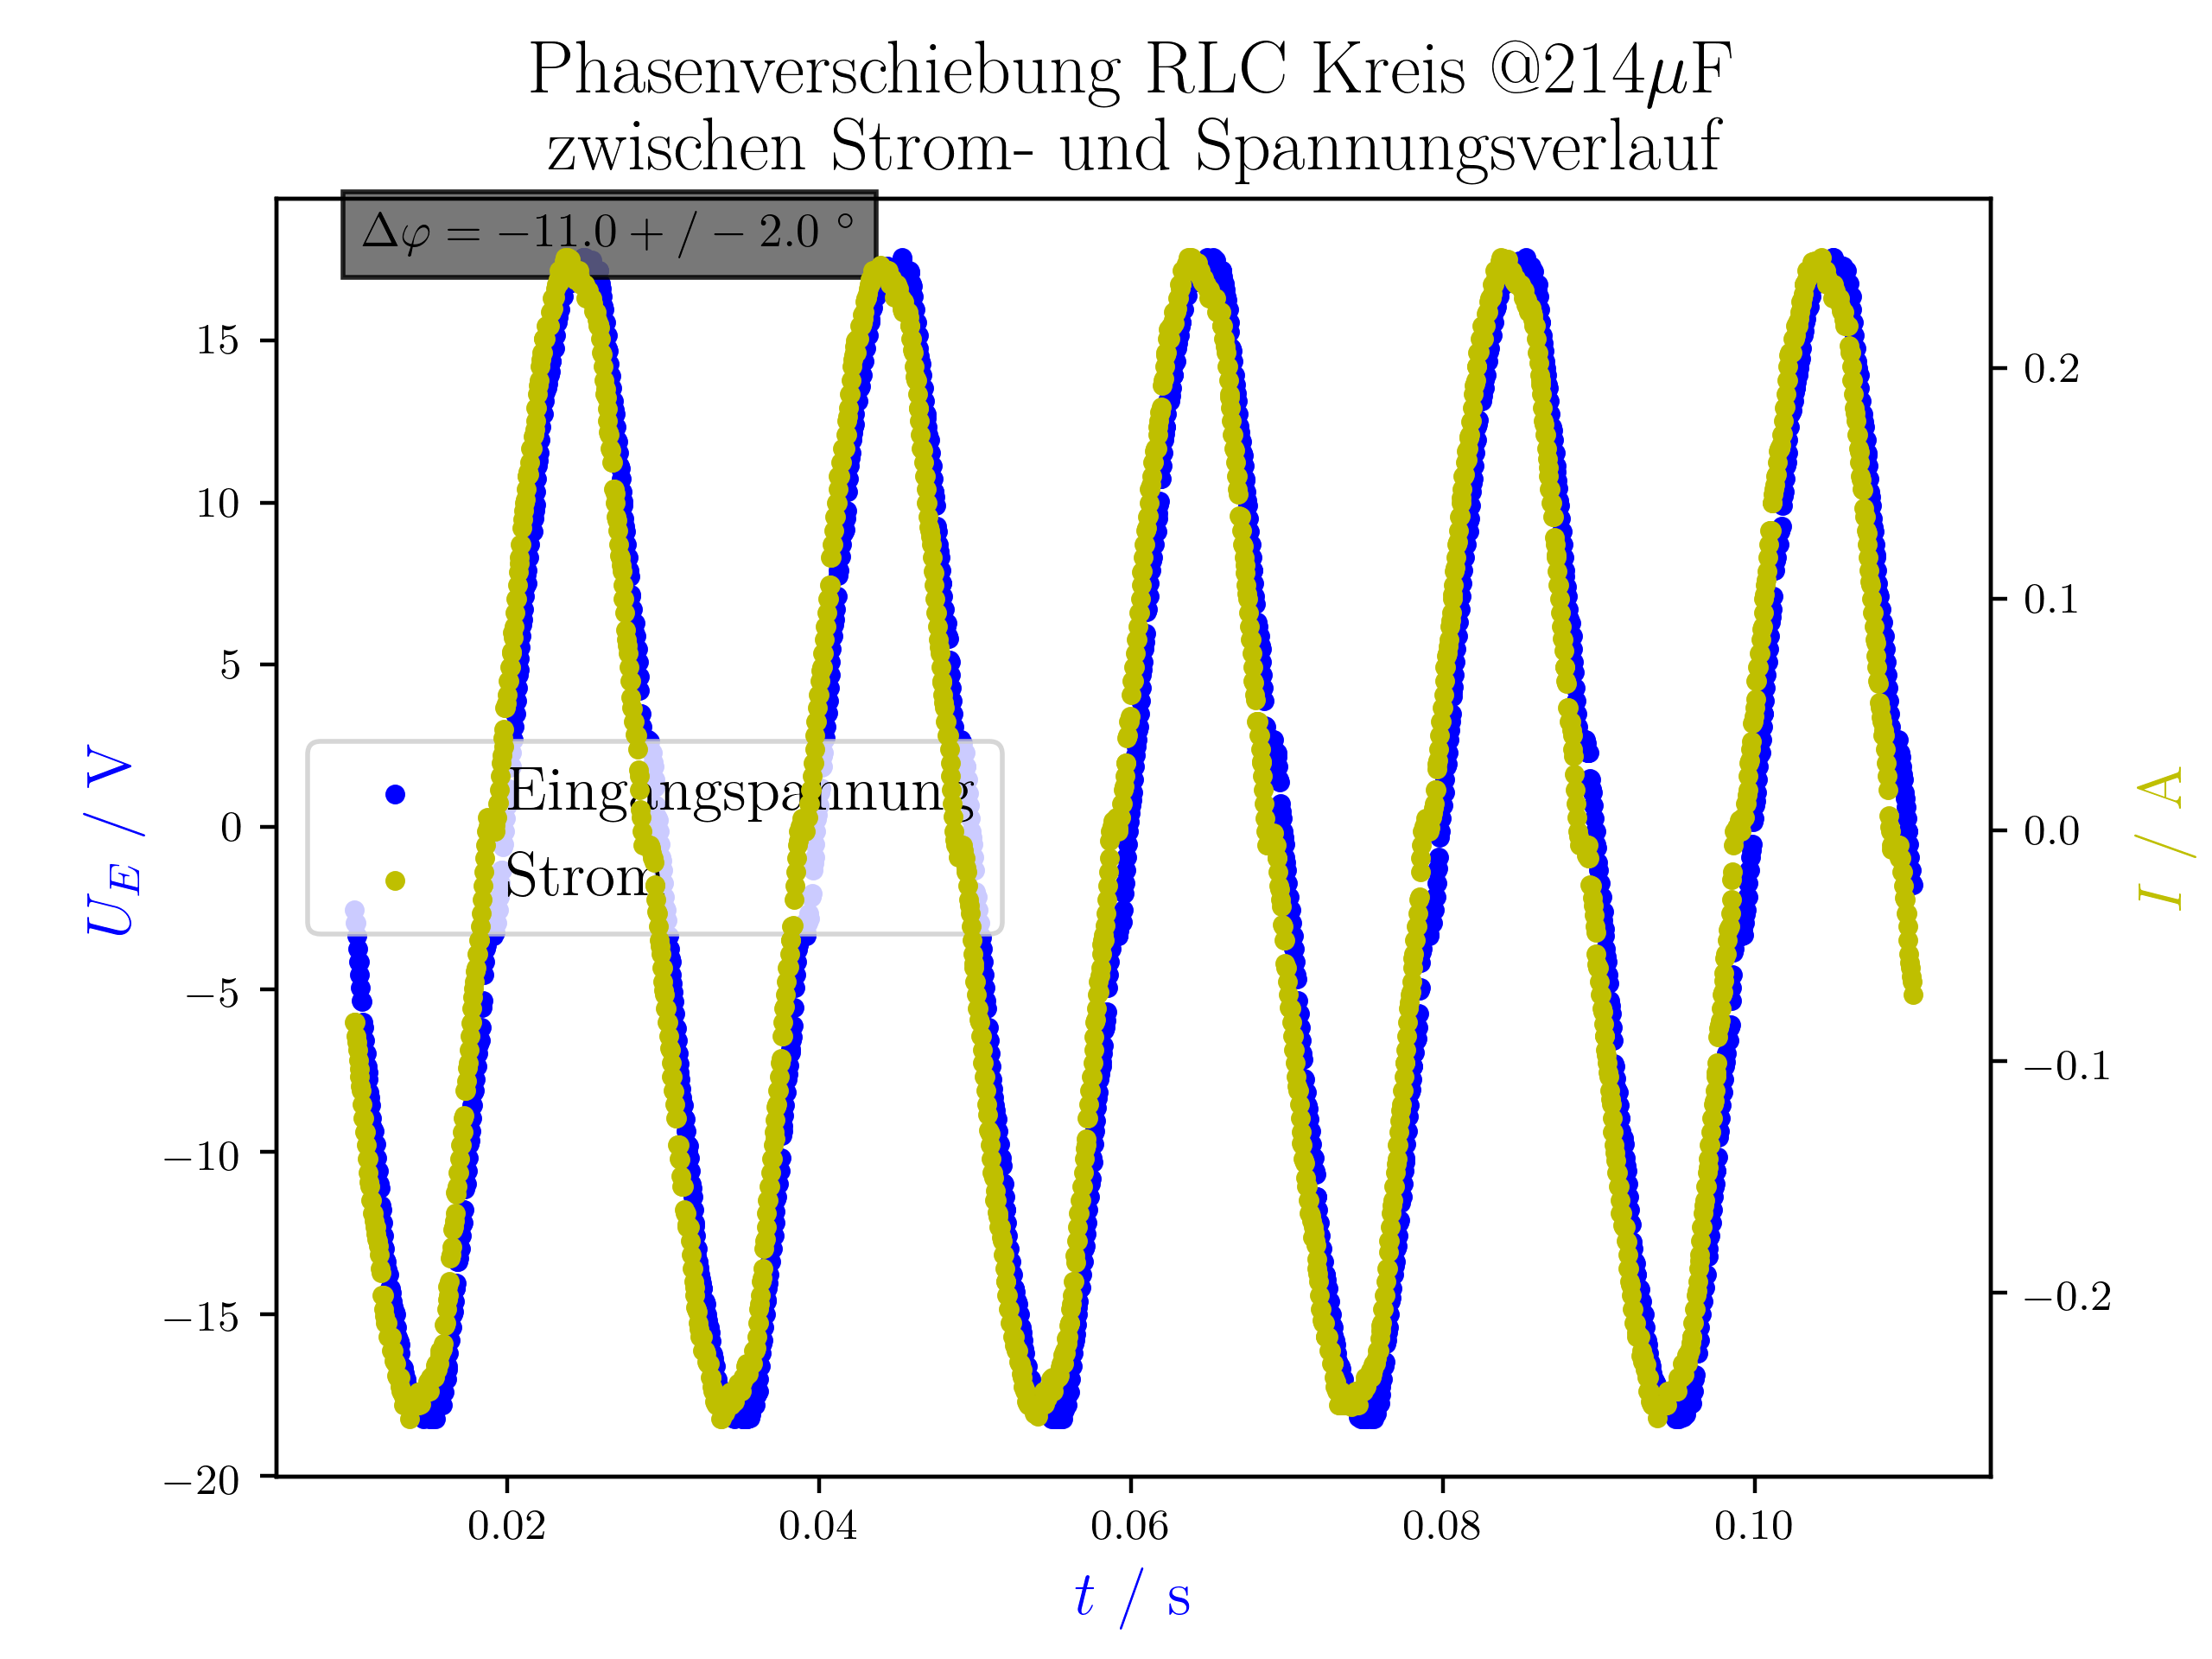
\includegraphics[width=\textwidth]{./figures/phaseleistung/Versuch6/phaseshiftrlc20.png}
		\captionof{figure}{Phasenverschiebung zwischen Strom und Spannung in RLC-Kreis bei einer Kapazität von 214 $\mu$ Farad}
		\label{fig:phaseshiftrlc20}
	\end{minipage}
\end{center}

Der entsprechende Wert der Phasenverschiebung am Oszilloskop beträgt -19.86°, siehe \autoref{fig:oszi_6_214} und ist wieder nicht im erhaltenen Fehlerintervall des errechneten Phasenversatzes enthalten.




\section{Diskussion}\label{disk}


\subsection{Anzeige von unterschiedlichen Spannungsmessinstrumenten}

Vergleicht man die verschiedenen Werte der Spannungen, die in \autoref{tab:1b} aufgelistet sind, wird klar ersichtlich dass keine absoluten Aussagen über die gemessenen Spannungen getroffen werden können, da diese stark vom Gerät abhängen.

\vspace{2mm}

Vor allem der Spannungswert des analogen Multimeters ist dabei jedoch mit Vorsicht zu verwenden, da dieser bei einer defekten Feder im inneren des Geräts leicht verfälscht werden kann. Dies kann beispielsweise durch deren Überspannung wegen einen falsch eingestellten Messbereich erreicht werden, was aufgrund des Alters des Geräts und der Tatsache, dass es von vielen Studenten benutzt wird, nicht ausgeschlossen werden kann.

\vspace{2mm}

Bei allen Geräten stimmt die aufgezeichnete Spannung jedoch größenordnungsmäßig mit dem theoretisch errechneten Wert überein.



\subsection{Phasenlage von Strom und Spannung an einem Kondensator}

Wie es die Theorie voraussagt, eilt der Strom im Kondensator der Spannung voraus, wie auch in \autoref{fig:kondensatorstromvor} ersichtlich.
Deckend dazu wurde ein negativer Phasenversatz vom Strom zur Spannung gemessen.


\subsection{Phasenlage von Strom und Spannung an einer Spule}

Wie es die Theorie voraussagt, eilt der Strom in der Spule der Spannung nach, wie auch in \autoref{fig:phaseshiftind} ersichtlich.
Deckend dazu wurde ein positiver Phasenversatz vom Strom zur Spannung gemessen.


\subsection{elektrische Leistung in einer RC-Schaltung}

Wie es zu erwarten war zeigt der Scheinleistungszeiger in den 1. Quadranten
aufgrund des Phasenversatzes, siehe \autoref{fig:powerdreieck_rc}

\begin{figure}[H]
	\begin{center}
		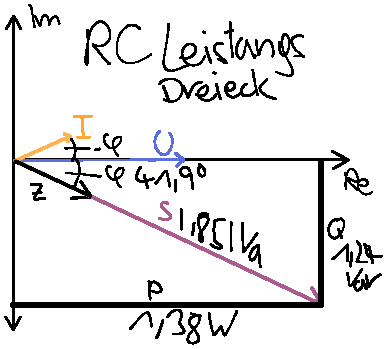
\includegraphics[width=0.55\textwidth]{./figures/rc_zeiger.pdf}
	\end{center}
	\caption{Hier sind die Gemessenen Werte der Leistungen im Zeigerdiagramm für den RC Kreis dargestellt worden}
	\label{fig:powerdreieck_rc}
\end{figure}


\subsection{elektrische Leistung in einer RL-Schaltung}

Wie es zu erwarten war zeigt der Scheinleistungszeiger in den 4. Quadranten
aufgrund des Phasenversatzes, siehe \autoref{fig:powerdreieck_rl}

\begin{figure}[H]
	\begin{center}
		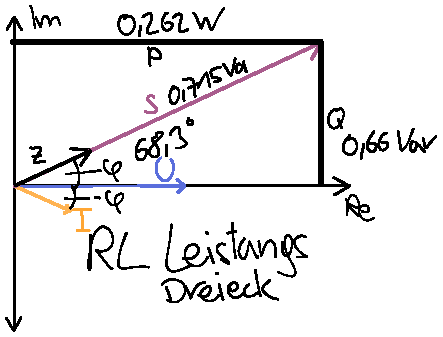
\includegraphics[width=0.55\textwidth]{./figures/rl_zeiger.pdf}
	\end{center}
	\caption{Hier sind die Gemessenen Werte der Leistungen im Zeigerdiagramm für den RL Kreis dargestellt worden}
	\label{fig:powerdreieck_rl}
\end{figure}


\subsection{Blindleistungskompensation eines induktiven Verbrauchers}

Weil die genaue Induktivität der Spule leider aufgrund von Zeitmangel Vorort,
trotz Versuchten Fehlerkorrekturen und erneuten Messungen, nicht richtig
bestimmt werden konnte und der Versuch fortgesetzt werden musste, konnte auch
die ideale Kapazität zur Kompensation im Vorhinein nicht nummerisch bestimmt
werden. Daher wurde mit verschiedenen Kapazitäten experimentiert und die
gesamte Kapazität immer erhöht. Weil das Powermeter durch nochmaliges
anschließen einen Wirkungsgrad von 99 \% anzeigte, wurde davon ausgegangen, die
ideale Kapazitätsverteilung gefunden zu haben. Dies stellte sich jedoch bei der
Auswertung als falsch heraus.

Ein Verbesserungsvorschlag wäre dadurch den Versuch mit der errechneten
Kapazität von 12,24 $\mu$ Farad zu wiederholen.


\subsection{Phasenversatz}

Im Laufe dieses Versuchs wurden die Phasenversätze auf verschiedene Arten
gemessen. Diese lieferten nicht immer gleiche Werte, wesshalb die erhaltenen
Winkel in folgender Tabelle nochmals aufgelistet sind. Die Unsicherheit des
abgelesenen Phasenwinkel am Oszilloskop wurde dabei als absolut angenommen,
weil keine genauen Informationen bezüglich des Fehlers bekannt sind und der
Wert ohnehin nur gegenübergestellt und für keine Rechnungen verwendet wird.

\begin{table}[H]
	\captionof{table}{erhaltene Werte für die Phasenverschiebungen\\ $\phi_{Oszi}$ \dots abgelesener Wert des Phasenwinkels am Oszilloskop  \\ $\phi_{er}$ \dots errechneter Wert für den Phasenwinkel \\ $\phi_{pow}$ \dots errechneter Wert für den Phasenwinkel anhand der vom Powermeter abgelesenen Daten \\ $C$ \dots bei Kondensator \\ $L$ \dots bei Spule \\ $RC$ \dots bei Serienschaltung von Widerstand und Kondensator \\ $RL$ \dots bei Serienschaltung von Widerstand und Spule \\ $RLC$ \dots bei der Schaltung für die Blindleistungskompensation bei entsprechender Kapazität}
	\begin{center}
		\begin{tabular}{|c|c|c|c|c|} \hline
			Schaltung   & $\phi_{Oszi}$ & $\phi_{er}$          & $\phi_{pow}$            \\ \hline
			C           & -86.25°       & \SI{-88(2)}{\degree} &                         \\ \hline
			L           & 86.00°        & \SI{81(2)}{\degree}  &                         \\ \hline
			RC          & -45.92°       & \SI{-41(2)}{\degree} & \SI{-41.8(15)}{\degree} \\ \hline
			RL          & 72.54°        & \SI{70(2)}{\degree}  & \SI{68(3)}{\degree}     \\ \hline
			$RLC_{47}$  & -51.42°       & \SI{-46(2)}{\degree} &                         \\ \hline
			$RLC_{147}$ & -24.04°       & \SI{-17(2)}{\degree} &                         \\ \hline
			$RLC_{214}$ & -19.86°       & \SI{-11(2)}{\degree} &                         \\ \hline
		\end{tabular}
		\label{tab:p_vgl}
	\end{center}
\end{table}

%-?

Vergleicht man die so erhaltenen Winkel erkennt man, dass diese zwar nicht
übereinstimmen aber in der gleichen Größenordnung sind.

\section{Zusammenfassung}

Anhand des Versuchs wurde gezeigt, dass verschiedene Messgeräte
unterschiedliche Werte für die selbe Spannung liefern.

\vspace{2mm}

Betrachtet man die erhaltenen Phasenwinkel aus \autoref{tab:p_vgl}, stellt man
fest, dass der Strom im Kondensator (sowohl bei C als auch bei RC) vorauseilt,
negativer Phasenwinkel, und bei der Spule nacheilt, positiver Phasenwinkel.

\vspace{2mm}

Wie ersichtlich sind die zeigt die Leistung in die Richtung des komplexen
Widerstandszeigen wie zu erwarten war.

\vspace{2mm}

Für die Kapazität der Spule L wurde folgender Wert errechnet.

\begin{align*}
	L = \SI{828(10)}{\milli\henry}
\end{align*}

Für die ideale Kapazität C wurde folgender Wert bestimmt.

\begin{align*}
	C = \SI{12.24(14)}{\micro\farad}
\end{align*}


\newpage

\printbibliography
\listoffigures
\listoftables
\end{document}



